
\documentclass[letterpaper,twocolumn,10pt]{article}
\usepackage{usenix2019_v3}
\usepackage{algorithmic}
\usepackage{algorithm}
\usepackage{listings}
\usepackage{pifont}
\usepackage{multirow}
\usepackage{graphicx}
\usepackage{caption}
\usepackage{xcolor}
\usepackage{booktabs}

% to be able to draw some self-contained figs
\usepackage{tikz}
\usepackage{amsmath}
\usepackage{cleveref}
\usepackage{subcaption}
\crefname{section}{§}{§§}
\Crefname{section}{§}{§§}

% new commands
\newcommand{\name}{CATFlow}

%-------------------------------------------------------------------------------
\begin{document}
%-------------------------------------------------------------------------------

%don't want date printed
\date{}

% make title bold and 14 pt font (Latex default is non-bold, 16 pt)
\title{\Large \bf \name{}: Data-Monistic Parallelism Plan Discovery for Distributed Training
}

%for single author (just remove % characters)
\author{
\vspace{-2em}
% {\rm Your N.\ Here}\\
% Your Institution
% \and
% {\rm Second Name}\\
% Second Institution
% % copy the following lines to add more authors
% % \and
% % {\rm Name}\\
% %Name Institution
} % end author

\maketitle

%-------------------------------------------------------------------------------
\begin{abstract}
%-------------------------------------------------------------------------------

As neural networks grow in size and complexity, distributed training across multiple devices becomes essential. An expressive abstraction is crucial for describing diverse parallelism plans to maximize hardware resource utilization. However, prevailing operator-centric abstractions fall short, as they fail to capture diverse data movement optimizations and data lifecycle management, lack mechanisms for the automatic discovery of new parallelism plans.

In this paper, we introduce \name{}, a framework with a novel abstraction that presents a key insight: defining parallelism spaces from a pure data-monistic perspective offers greater expressiveness and completeness than operator-centric approaches. \name{} is built upon three fundamental concepts: tensors, space-time coordinates, and their relationships—formalized as constraints. It also provides a set of primitives for constructing and manipulating these elements, enabling the description of diverse schedules and the co-optimization of computation and data movement. A key advantage of \name{} is its capacity to explicitly encode constraints on spatial dataflow trajectories and precise tensor lifecycles through these primitives, forming a space that can contain unforeseen strategies. This facilitates systematic searches within this constrained optimization space to discover new, efficient parallelism plans. Using a constraint-based potential-descent algorithm, \name{} has discovered novel parallel-training solutions such as ZeRO-3.5 and ZeRO-4, which achieve up to 39.1\% performance improvement over ZeRO-3 and 36.6\% memory reduction compared with ZeRO-2 across hardware configurations, as well as new offloading strategies that boost throughput by up to 89.4\%. With these capabilities, \name{} contributes to democratizing LLM training in resource-constrained scenarios.


% effectively covering operator schedulings like 3D parallelism and 1F1B, co-optimizations of computation and data movement like FSDP, and dataflow-driven strategies like WeiPipe—capabilities that extend beyond existing frameworks.

% Instead of searching configurations within a predefined or expert-crafted parallelization mechanism, \name{} enables explicitly adding constraints to spatial dataflow trajectories and tensor lifecycles through its primitives, thereby facilitating the search within the constrained space for discovering new parallelization mechanisms. 


% in resource-constrained scenarios 
\end{abstract}

\vspace{-0.5em}
\section{Introduction}
\label{sec:intro}

Deep Neural Networks (DNNs), particularly large language models (LLMs), have achieved advanced performance across a wide range of domains~\cite{deepseekai2025deepseekr1, openai2024gpt4, brown2020language, silver2017mastering}. However, the efficient training of large-scale models necessitates substantial resources, frequently surpassing the capabilities of one device~\cite{narayanan2021efficient}. Consequently, distributing training across multiple devices is crucial~\cite{duan2024efficient, athlur2022varuna}. The core challenge lies in identifying an efficient parallelism plan for distributed training. An NN model can be formally modeled as a computational graph~\cite{lin2023songc}, where nodes represent either data storage (tensors) or computations (operators), and directed edges represent dependencies between nodes. A parallelism plan specifies the distribution and scheduling of storage and computation in both space (device placement) and time (execution order)~\cite{qiu2025moirai, huang2019yugong, lin2024nnscaler, xu2021gspmd}. The space of feasible parallelism plans is vast, and the problem of determining an optimal plan is NP-hard~\cite{liu2024aceso}.

Due to the immense search space and complex constraints, distributed training optimizations often rely on meticulously designed prallelism paradigms that incorporate domain expertise. Examples include Megatron-LM~\cite{shoeybi2019megatron, narayanan2021efficient}, which incorporates parameterized parallelism paragidms known as data, tensor, and pipeline parallelism (DP, TP, PP, collectively termed 3D parallelism) to support Transformer-based models. Alternatively, systems like Piper~\cite{tarnawski2021piper} and Alpa~\cite{zheng2022alpa} adopt a hierarchical search, first determining a plan for pipeline (inter-operator) parallelism, then optimizing tensor (intra-operator) parallelism within each stage. A common pattern across these methods is to first define a specific parallelism paradigm (e.g., 3D or SPMD parallelism) and then perform an efficient hyperparameter search within that paradigm—for instance, tuning the degrees of data, tensor, and pipeline parallelism.
% which organize parallelization choices into a two-level hierarchical space termed staged single-program, multiple-data (SPMD). In this approach, the system 

% These approaches typically first define a parallelization paradigm and subsequently perform a parameter search to find the best configuration, such as the degree of DP, TP, and PP. 


\begin{table*}[t!]
\small
\centering
\setlength{\tabcolsep}{4pt}
\caption{High-level comparison of different methodologies.}
\vspace{-0.5em}
\label{tab:landscape}
\begin{tabular}{p{0.14\linewidth}p{0.26\linewidth}p{0.26\linewidth}p{0.26\linewidth}}
\toprule
\textbf{Feature} & \textbf{Classical} (e.g., Megatron-LM~\cite{shoeybi2019megatron}) & \textbf{nnScaler~\cite{lin2024nnscaler}} & \textbf{\name{}} \\
\midrule
\textbf{Fundamental view} & \textbf{Strategy-centric:} fixed library of named strategies (e.g., DP, PP, TP) & \textbf{Operator-centric:} define strategy by operator behaviors & \textbf{Data-monistic:} define strategy by data space-time trajectories \\
\textbf{Space definition / Prim. semantics} & \textbf{Fixed templates:} combination of existing paradigms (e.g., 1F1B, 3D) & \textbf{Constructive:} default-deny, explicitly permit; build form zero. & \textbf{Subtractive:} default-allow, explicitly forbid; carve from universal set\\
\textbf{Completeness} & combination of built-ins &  complete for computation scheduling & covering computation, storage, and communication co-optimization \\
\textbf{Expressiveness} & combination rules of built-ins & custom operator schedules, no data-centric optimizations. & fine-grained control over tensor lifecycle and events \\
\textbf{Searchability} & \textbf{Parameter search} & \textbf{Para. search in user-defined space} & \textbf{Automatic strategy discovery} \\
\textbf{Dataflow handling} & Implicit and fixed by chosen strategy & Implicit side-effect of operator & Explicit and first-class citizens \\
\bottomrule
\end{tabular}
\vspace{-1em}
\end{table*}

While many studies~\cite{tarnawski2021piper, zheng2022alpa, um2024metis, ge2024enabling, sun2024adapipe, isaev2023calculon, strati2025sailor, zhu2025mist, wang2019supporting} aim to find optimal hyperparameter configurations within well-established parallelism paradigms, recent work such as nnScaler~\cite{lin2024nnscaler} advocates for a more flexible approach. It provides domain-specific primitives that enable experts to construct customized parallelism plans, thus creating an abstraction framework for expressing more flexible solutions and unlocking further optimizations for large model training, e.g., 3F1B for AlphaFold2~\cite{Jumper2021}. Specifically, nnScaler's abstraction framework is predominantly operator-centric, introducing three primitives—\texttt{op-trans}, \texttt{op-assign}, and \texttt{op-order}—to specify operator placement, transformation, and execution order. Focusing primarily on operator scheduling, nnScaler enables the description of parallelism plans that extend far beyond the scope of traditional 3D or SPMD approaches.

% This paradigm recognizes that variations in hardware, workload characteristics, and expert knowledge can lead to distinct preferred strategies, 
% Experts define novel strategies with their designed patterns and search configurations.

% However,  nnScaler still faces two limitations. First, they either define rigid strategy spaces or lack completeness in strategy specification, making it hard to capture more potential opportunities. 

Although nnScaler~\cite{lin2024nnscaler} represents a significant advance, capable of describing most existing training plans and new expert-crafted parallelism paradigms, existing approaches remain limited in expressing optimizations that require coordinated data movement and lifecycle management, such as BPipe~\cite{kim2023bpipe}, WeiPipe~\cite{lin2025weipipe}, complex cross-mesh resharding~\cite{zhuang2023optimizing}, and ZeRO-3.5 \& 4 (new strategies discovered in this work). This limitation hinders the ability to fully exploit hardware resources. The root cause is that prior operator-centric abstractions~\cite{lin2024nnscaler, lin2024tessel, zheng2022alpa} typically build on predefined dataflow assumptions and cannot effectively describe flexible spatial dataflow trajectories and fine-grained tensor lifecycle. Consequently, many potential optimization opportunities cannot be expressed or discovered due to this incompleteness.
% of expressive power.

% Second, the quality of this pre-designed space is a critical determinant of the achievable performance of these frameworks, which are limited to automated search within a fixed strategy space; search algorithms select among efficient configurations and parameter settings (e.g., partition sizes, device assignments, execution order) rather than enabling the automatic discovery of unforeseen strategies.

% For methods that define strategies using domain-specific primitives, their expressiveness is constrained by the underlying abstractions and specifications. Existing approaches are predominantly operator-centric. For instance, nnScaler~\cite{lin2024nnscaler} introduces three primitives—\texttt{op-trans}, \texttt{op-assign}, and \texttt{op-order}—for specifying operator behaviors. These approaches focus on computation and implicitly bind data movement to operator scheduling. We present a core contrary insight: adopting a \textbf{data-monistic} perspective yields a more expressive and complete abstraction for strategy-space construction, in which parallelization plans are defined by describing the trajectory of data and imposing constraints on its movement. From this viewpoint, computation is implicitly represented as a \textbf{constraint} on dataflow; that is, its occurrence means all required data must meet at the same device, and the scheduling of computation can be deduced naturally from the constraints that govern data movement.

We therefore present a core contrary insight in this work: a \textbf{data-monistic} perspective offers a more expressive and complete abstraction for parallelism plans description and strategy space construction. In this view, plans are defined by describing the trajectory of data and imposing constraints on its movement. From this vantage point, computation is implicitly represented as a \textbf{constraint} on dataflow, specifically, that all required data must meet at the same device. Consequently, the scheduling of computation follows naturally from the constraints governing data movement.

Building on this insight, we present \name{}—a new framework for describing, generating, and searching for more advanced distributed-training plans. Its core is an abstraction centered on a single entity: the constraint-aware tensor (CAT). The constraints associated with each tensor specify its space-time coordinates—that is, when and where the tensor resides. On top of this representation, \name{} provides a set of primitives for manipulating CATs to constrain parallelism plans that coordinate data movement and computation, including tensor distribution, dependency management, and strategy-space delineation primitives.

% \begin{table*}[t]
% \small
% \centering
% \setlength{\tabcolsep}{4pt}
% \caption{High-level comparison of paradigms.}
% \label{tab:landscape}
% \begin{tabular}{llll}
% \toprule
% Feature & Traditional & nnScaler & \name{} \\
% \midrule
% Fundamental view & Strategy-centric & Operator-centric & Data-monistic \\
% Space definition & Fixed templates & Constructive & Declarative \\
% System role & Parameter search & Template search & Strategy discovery \\
% Expressiveness & Low (built-ins) & Medium (op-schedules) & High (data \& op) \\
% Dataflow handling & Implicit & Implicit & Explicit \\
% \bottomrule
% \end{tabular}
% \end{table*}

\name{}'s abstraction paves the way for addressing another important problem: prior work limits automated search to tuning hyperparameters (e.g., partition sizes, device assignments, execution order) within a fixed, manually crafted parallelism space, preventing the automatic discovery of \textbf{unforeseen parallelism plans}. In contrast to predefined search spaces, \name{} employs declarative, \textbf{subtractive} primitives to \textbf{carve} a \textit{universal} design space through constraints. While traditional search frameworks depend on constructive primitives, mandating that users define what a parallelism plan should be, \name{} inverts this logic: designers simply state what a parallelism plan should not be. This reductive methodology generates a search space spanning known and unknown designs, fostering the discovery of advanced parallelism plans. Coupled with a data-monistic perspective, it delivers a unified, high-resolution strategy landscape that increases optimization tractability and supports seamless parallelism plan transitions during search. Building on this foundation, we introduce a constraint-based potential-descent algorithm capable of discovering novel parallelism plans. Table~\ref{tab:landscape} summarizes the key distinctions between \name{} and prior approaches.

\name{}'s core contributions are summarized as follows:

1. \textbf{Data-Monistic Abstraction and Parallelism Space:} We introduce \name{}, a framework featuring novel abstractions and primitives for constructing spaces of parallelism plans in distributed NN training. From a data-monistic perspective, \name{} enables the explicit and complete specification of plans governing both computation and data movement. In contrast to existing operator-centric methods, it unlocks a strictly larger parallelism-plan space.

2. \textbf{Automatic Discovery of Novel Training Plans:} By using \name{}'s unified abstractions to reductively carve a training-plan search space, we establish a foundation for the automated discovery of unforeseen training plans, in conjunction with an efficient potential-descent search algorithm.
% . We thus introduce a hierarchical potential descent algorithm that operates within this space to uncover unforeseen parallelization paradigms.

3. \textbf{Invention of New Plans for Large Model Training:} Based on \name{}, we present new, efficient distributed training plans for resource-constrained scenarios that surpass state-of-the-art, manually designed solutions. These include new ZeRO strategies, ZeRO-3.5 \& 4 that achieve the memory efficiency of ZeRO-3 and performance approaching that of ZeRO-2 (up to 39.1\% improvement over ZeRO-3), as well as new offloading strategies that boost throughput by 89.4\%.

\section{Background \& Motivation}

\subsection{Parallelism Paradigms \& Plan Search}

% 首先说有很大的搜索空间
% 然后介绍了了DP, TP, PP以及3D并行
% 介绍一下Tessel的PP, Megatron的3D并行search space, Alpa和Piper的staged SPMD
% 介绍一下exiting search spaces存在limitations, 这样的predefined的search space是针对固定的workload准备的, 对于更大范围的workload来说，不够通用，会丢掉很多优化机会，比如说AlphaFold2的3F1B和embedding层的low computation utilization问题

A \textit{parallelism plan} specifies how a model and the associated data are partitioned and scheduled across multiple devices, including the distribution of tensors (data), operators (computations), and their temporal order. The challenge lies in the vast combinatorial space of possible plans, and finding an optimal solution is NP-hard~\cite{liu2024aceso}. Existing search methods commonly construct a search space from handcrafted, parameterized \textit{parallelism paradigms} and then tune parameters within that space to efficiently find good plans. Typical \textit{parallelism paradigms} include \textit{data parallelism} (DP), \textit{tensor parallelism} (TP), \textit{pipeline parallelism} (PP), and \textit{sequence parallelism}~\cite{li2023sequence} (SP), and \textit{3D(4D) parallelism} integrates DP, TP, PP (and SP) together. Megatron-LM~\cite{shoeybi2019megatron, narayanan2021efficient} is a representative framework that combines DP, TP, and PP for Transformer training. Subsequent systems like Piper~\cite{tarnawski2021piper} and Alpa~\cite{zheng2022alpa} extend 3D parallelism with staged SPMD (single program multiple data). While effective, these systems often rely on fixed pipeline schedules~\cite{qi2024zero}, such as 1F1B~\cite{huang2019gpipe}, and overlook the potential of fine-grained micro-batch scheduling. Tessel~\cite{lin2024tessel} addresses this limitation by optimizing micro-batch scheduling for a given operator placement.

% , which first searches for a PP plan and then an SPMD plan within each stage

To enable automatic parallelization, existing training systems typically construct parameterized search spaces from predefined \textit{parallelism paradigms}. Consequently, the quality of discovered \textit{parallelism plans} depends strongly on the quality of these predefined spaces. As shown by nnScaler~\cite{lin2024nnscaler}, such fixed spaces can miss important optimization opportunities. For example, AlphaFold2~\cite{jumper2021highly} requires three forward passes before each backward pass, a pattern that cannot be efficiently handled by 1F1B pipeline schedules. In multilingual LLMs~\cite{ni2022sentence}, applying standard 3D parallelism/staged SPMD can force large embedding tables to occupy excessive devices, leading to poor computational utilization. These cases demonstrate how hand-crafted, fixed search spaces fail to capture novel optimization patterns in evolving workloads.


\vspace{-.5em}
\subsection{Construction of New Parallelism Plans}

% 为了解决上述问题，recent research, especially nnScaler, 希望能够提出一种更灵活的方式来构建parallelization plan space, enable domain experts to find more effective training plans for their models. nnScaler中主要提出了三种primitives: nnScaler introduces \texttt{op-trans}, \texttt{op-assign}, and \texttt{op-order} to specify operator partitioning, spatial placement, and temporal scheduling, respectively. 通过这三种基本的primitives可以定义广阔的并行空间, 再结合nnScaler中所提出的powerful的constraint表示，which can prune the search space defined by primitives, nnScaler可以表示现有工作所不能包含的一系列并行search space，比如特殊的PP strategy for alphafold with 3 forward process and 1 backward, stage_spmd + 特殊的mapping方式for specific ops, like embedding in Language models, 语序不同的PP stage share devices. 

% 但是，尽管nnScaler的强大能力，我们发现他所能够表示的并行搜索空间仍然是有限，因为neglect掉了 the crucial role of data movement and the potential for \textbf{co-optimizing computation and dataflow}. 我们主要关注两类search space that cannot be expressed  by existing works. 首先是standalone dataflow 优化，for example, 在nnScaler中，提出了and so each device holds only one split operator. However, we observe that sometimes multiple split operators can share a single device and compute in a streamlined manner, resulting in fewer devices required for each pipeline stage and less memory consumption. Although the streamlined computing of multiple split operators may slow down the computing process, the reduced communications across fewer devices can lower cost and speed up the overall process. Normally, the streamlined computing的结果应该在本地reduce，但实际上，nnScaler无法限制数据移动的轨迹，如果我在每一次计算过程之后都在不同的device之间去做reduce，显然会引起更大的通信代价，这说明如果我们只关注operator本身的parallelization, 而忽略了dataflow相关的organization以及scheduling的话, 会丢失很多优化的机会，并且也无法准确定义完整的并行行为。

% To address the limitations of existing parallelism paradigms, 
Recent research has introduced a flexible abstraction framework for constructing diverse \textit{parallelism plans}. Specifically, nnScaler~\cite{lin2024nnscaler} defines three core primitives for operator partitioning, spatial placement, and temporal ordering. By composing these primitives with user-specified constraints, nnScaler can express a broader spectrum of \textit{parallelism plans} than prior approaches, such as specialized pipeline schedules (e.g., 3F1B for AlphaFold2) and staged SPMD with customized operator mappings (e.g., embedding). Nevertheless, existing operator-centric abstractions introduce inherent limitations: they typically rely on predefined dataflow assumptions and cannot effectively handle flexible spatial dataflow and tensor lifecycle management.

In modern distributed training, performance depends not only on how computation is parallelized but also on how data is orchestrated and moved~\cite{huang2019yugong, qiu2025moirai, zhu2025mist, kim2023bpipe, lin2025weipipe, xu2021gspmd}. Many state-of-the-art optimizations are explicitly data-driven, e.g., ZeRO~\cite{rajbhandari2020zero, zhao2023pytorch}, activation checkpointing~\cite{chen2016training}, and offloading~\cite{ren2021zero}, which tightly coordinate parameter sharding, prefetching, asynchronous communication, and conditional transfers with computation scheduling. However, operator-centric frameworks~\cite{lin2024nnscaler, lin2024tessel} typically treat data movement as an implicit byproduct of operator placement and ordering, lacking mechanisms to explicitly control or co-optimize dataflow; consequently, they cannot express \textit{parallelism plans} that jointly orchestrate computation and data movement~\cite{zhuang2023optimizing} or require complex tensor lifecycle management~\cite{kim2023bpipe, lin2025weipipe}. This limitation prevents the discovery and representation of a critical class of high-performance \textit{parallelism plans}, motivating a more expressive, data-centric abstraction.

% \subsection{Limitations of Operator-Centric Abstractions}

% In modern distributed training, performance is increasingly dictated not just by how computation is parallelized, but by how data is managed and moved~\cite{huang2019yugong, qiu2025moirai}. A growing number of advanced optimizations focus explicitly on dataflow, such as Fully Sharded Data Parallelism (FSDP)~\cite{rajbhandari2020zero}, which coordinates parameter sharding with computation, or sophisticated memory-saving techniques like activation recomputation and offloading. These strategies involve complex data trajectories—prefetching, asynchronous communication, and conditional data movement—that are tightly coupled with the computation scheduling.

% However, existing operator-centric frameworks~\cite{lin2024nnscaler} struggle to express these data-centric optimizations. By treating data movement as an implicit side-effect of operator placement and scheduling, they lack the vocabulary to explicitly control or co-optimize dataflow. For example, nnScaler cannot express optimizations that tightly coordinate computation and data movement, such as FSDP, or complex dependency management in recomputation strategies. This limitation prevents existing systems from discovering or representing a critical class of high-performance parallelization plans, motivating the need for a more expressive, data-centric abstraction.


\vspace{-.5em}
\section{Abstraction with Constraint-Aware Tensor}
\label{sec:abstraction}

% Distributed training requires not only partitioning computation but also controlling data movement and its coordinated scheduling. 

To address the limitations of operator-centric abstractions, \name{} introduces a new representation: the \textbf{constraint-aware tensor (CAT)}, associated with three tightly coupled concepts: \textit{Tensor}, \textit{Space-Time Coordinate}, and \textit{Constraint}. 
% 之所以不在此处区分强约束与弱约束，是因为CATFlow的核心目标在于帮助用户构建策略空间，而非直接指定具体的并行策略。
% 搜索算法的任务是在该策略空间内寻找最优解，而不是突破或打破这些约束，因此强弱约束的区分在此意义不大。
% 此外，所谓的强约束通常对应于计算相关的约束，其作用与下文所述的Inter-tensor constraint基本一致。

\textbf{\textit{Tensor}}: Represents a data block within the computation graph, including both persistent model parameters and transient intermediate results, like activation values.

\textbf{\textit{Space-Time Coordinate}}: Denotes the location (device) and temporal position. Rather than using physical time, the temporal coordinate is defined by Lamport logical time~\cite{lamport2019time}, which reflects the execution order (see \cref{sec:dependency}).

\textbf{\textit{Constraint}}: Specifies the relationships between tensors and their space-time coordinates, determining where (device/location) and when (temporal order) a tensor exists or is operated upon. This enables explicit modeling of both data placement and execution timing for each tensor instance. 
% Constraints can be further categorized as:
\vspace{-.35em}
\begin{itemize}
    \item \textbf{Intra-tensor constraint}: Restricts the trajectory of a single tensor across different space-time coordinates, governing its movement and lifecycle.
    \vspace{-.35em}
    \item \textbf{Inter-tensor constraint}: Ensures that multiple tensors coincide at the same space-time coordinate, thereby enabling computation or enforcing temporal relationships.
\end{itemize}
\vspace{-.35em}

% This abstraction enables fine-grained control over tensor partitioning, assignment, reduction, ordering, etc., supporting expressive strategies beyond operator-centric approaches
\begin{figure}[t]
  \centering
  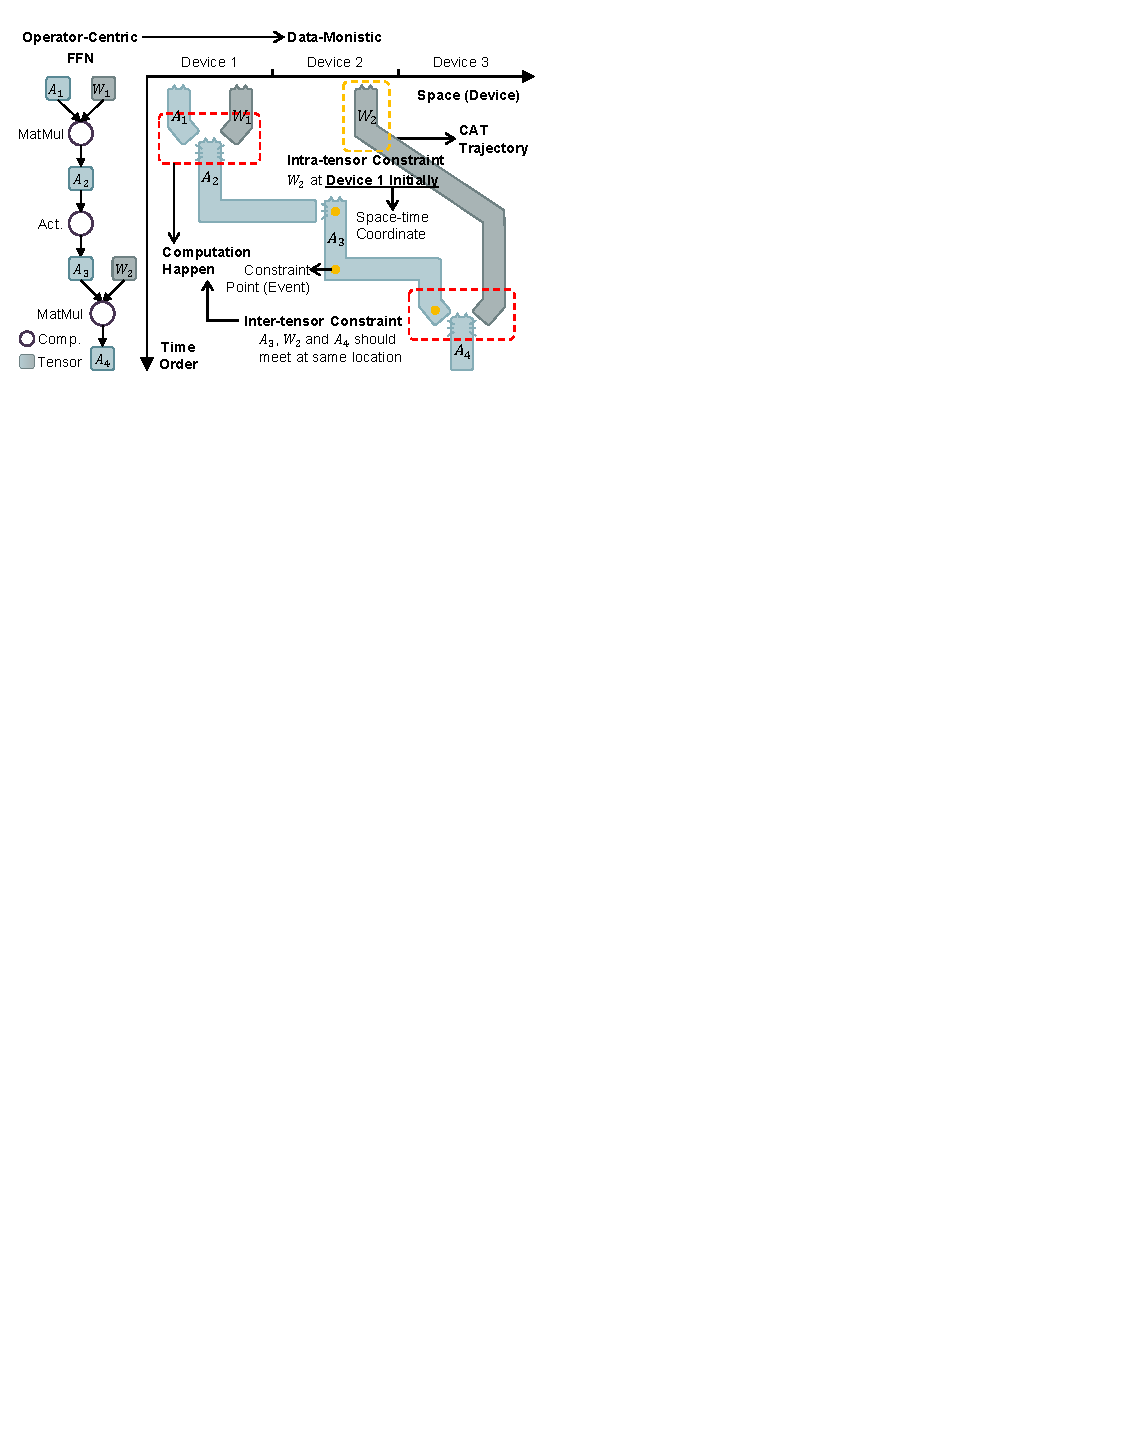
\includegraphics[width=1\linewidth]{figures/abstractions.pdf}
  \vspace{-1.3em}
  \caption{Illustration of the data-monistic abstraction: a baisc FFN layer in Transformer. Each tensor is annotated with constraints that explicitly specify its space-time coordinates.}
   \vspace{-1.2em}
  \label{fig:abstractions}
\end{figure}

% Figure \ref{fig:primitives}(a) illustrates the difference between operator-centric and dataflow-centric perspectives. From the dataflow perspective, everything in the graph is represented by the \textit{flow} of data. Each tensor is not merely a static data block in memory, but a dynamic process. The \textit{head} of the arrow in Figure \ref{fig:primitives}(a) represents the beginning of tensor generation, and the \textit{tail} represents the completion of data generation. If the flow of \texttt{tensor1} and the flow of \texttt{tensor2} meet, the generation of \texttt{tensor3} will naturally be triggered. This dataflow perspective for describing NN workloads forms the foundation of our dataflow-centric primitives.


% 在之前的版本中，event 被放在 dependency 那一节介绍，但从逻辑上看，constraint point 应作为完整抽象描述的一部分，应该在此处介绍。
% 但这样做也有一些风险：
% 1. generation 和 consumption event 实际上就代表了计算。如果我们的抽象对其进行了精细描述，实际上等价于直接描述了计算的调度。我们的做法是用一种统一的方式来描述计算与数据流调度的超集。但在文章中不宜直接这样解释，否则会削弱“二元对立”的叙事，影响创新性的判断。
% 2. 末尾的 event 更准确地说代表数据释放，而非消费。
% 3. 在此处介绍 event 机制可能会增加文章前期的阅读难度，使 monistic 抽象显得复杂（而此处又无法展示这种复杂性带来的好处）。但总体来看，这一想法还是比较直接的。
% 4. 不同的 event 蕴含不同的“细节”。例如我们将 move 放在发送方而非接收方，那么如何确定发送目标？可通过下一个 event 的空间坐标判断。另外，约束向量并未描述设备间通信带宽和延迟等信息。
% 5. 关于 move 实现的一个潜在冲突：有时我们不希望指定两个约束点之间的具体路径（留给搜索算法探索），即两个约束点之间搜索算法可以插入新的约束点。这种“路径未知性”可能与 move 默认发送到下一个约束点所在设备的语义存在一定冲突。

A CAT is more than a static data block—it encapsulates both the data themselves and the dynamic trajectory of their generation, movement, and release. We use a series of \textbf{constraint points}, which form a \textbf{constraint vector}, to describe the space-time trajectory of a CAT. During implementation, these constraint points are realized as \textbf{events} that operate on the tensor. For instance, the first and last points in the constraint vector represent the CAT's generation and release events, respectively, and intermediate points typically signify movement events between devices. Fig.~\ref{fig:abstractions} demonstrates how a FFN layer is represented in the CAT abstraction. In this case, the trajectory of tensor $A_3$ is represented by the following constraint vector: $\mathbf{C}_{A_3} = [(\mathrm{Device}_2, t_1), (\mathrm{Device}_2, t_2), (\mathrm{Device}_3, t_3)]$. $\mathbf{C}_{A_3}$ also signifies its lifecycle: generated on Device 2 by consuming $A_2$, and sent to Device 3, where it is consumed to produce $A_4$.

This data-monistic abstraction is strictly more expressive than operator-centric approaches. Instead of treating data movement as an implicit side effect of operator scheduling, \name{} defines computation as a consequence of data colocation: an operator executes when its input tensors meet at the same space-time coordinate to generate output tensors in place. By describing the trajectory of data, we uniformly define the scheduling of computation, storage, and communication. This reversal allows \name{} to represent any operator-centric plan, plus a wider range of parallelism plans that co-optimize computation and dataflow and manage complex data dependencies, lifecycle management, and movement.

\section{Primitives for Abstraction Manipulation}
\label{sec:primitives}

% While directly manipulating each tensor's fine-grained constraints offers maximum flexibility, doing so for an entire parallelization plan is both tedious and error-prone. 

To simplify the construction of data-monistic abstractions, \name{} provides six high-level primitives and corresponding mechanisms. These primitives serve as tools for building parallelism spaces, connecting tensors and space-time coordinates through constraints to generate valid representations within \name{}. They can be categorized into three groups:

\textbf{Tensor distribution primitives} include \texttt{split}, \texttt{assign}, \texttt{copy}, and \texttt{reduce}, which manage the spatial distribution of tensors. Together they define how data are partitioned, placed, and moved across devices.

\textbf{Dependency management primitives} include \texttt{order} and \texttt{redirect}, which govern the logical temporal ordering of events. \texttt{order} enforces specific ordering between events, whereas \texttt{redirect} transfers dependencies across tensors.

\textbf{Strategy-space delineation mechanisms} declaratively define and constrain the search space. For instance, a \texttt{domain} specifies the permissible range of values for a primitive's configuration (e.g., space-time coordinates), and \texttt{not} can explicitly exclude certain parallelism plans.

\subsection{Glance over Primitives with ZeRO}
\label{sec:primitives_glance}

ZeRO~\cite{rajbhandari2020zero, zhao2023pytorch} is a parallelism plan that builds upon DP to reduce memory usage. It achieves this by sharding the model parameters, gradients, and optimizer states across all available devices. The sharding strategy consists of tiered levels of ZeRO (Zero Redundancy Optimizer)~\cite{rajbhandari2020zero}: ZeRO-1 shards optimizer states, ZeRO-2 adds gradient sharding, and ZeRO-3 (FSDP~\cite{zhao2023pytorch}) also shards parameters for maximum memory savings. From an operator-centric perspective, these variants appear identical if dataflow management is treated as a side effect of operator scheduling. Algorithm~\ref{alg:fsdp} shows how \name{}'s primitives can represent the core of ZeRO variants. Specifically, the following primitives are used:

% During the forward pass, each device gathers the full parameters to perform computation, then discards them, retaining only its shard. In the backward pass, gradients are computed locally and immediately reduced and sharded to target devices via reduce-scatter, avoiding redundant storage. 

% 关于Primitive的相关细节，若需展开，建议放在附录中说明：
% 1. 在abstraction部分已提到，CAT的轨迹由其constraint vector中的各事件点控制。因此，理论上原语应直接操作事件点而非tensor。文中以tensor为原语输入输出，实为语法糖：若tensor无时空约束，则视为静态数据块，原语操作直接作用于其本体；若tensor有时空约束，默认其位于同一device，原语操作亦无歧义。但若tensor轨迹跨设备，则split和copy的结果难以直观界定，若需定义可参考第2点。此外，reduce原语可理解为作用于tensor最后一个事件点的状态。
% 2. 关于约束的继承：若对已具复杂约束向量的tensor执行split或copy，合理做法是新生成的向量不继承原有约束向量。
% 3. 关于依赖的继承：split和copy所得tensor继承原输入的依赖关系。split原语会根据切分数据的具体部分判断应保留的约束，输出约束需自动化编译过程依据“最近的等价数据块”自动判定。
% 如何处理约束与依赖的继承机制，使CATFlow既不产生声明矛盾，也不影响自动化优化，是原语设计的一个挑战。
% 4. 原语的具体处理细节及默认行为，如split的切分向量维度设计、copy的路径指定、reduce的操作类型（如有）等。

\texttt{dst\_tensor=copy(src\_tensor,copy\_num,path)} copies the \texttt{src\_tensor} into \texttt{copy\_num} replicas. The \texttt{path} parameter can specify the copy trajectory, e.g., $W_1^2$ is copied from $W_1$, $W_1^3$ is copied from $W_1^2$, etc. (Fig.~\ref{fig:primitive_intro1}(a)).

\texttt{split\_tensors=split(tensor,split\_vector)} partitions a \texttt{tensor} into multiple sub-tensors (\texttt{split\_tensors}) according to \texttt{split\_vector} (Fig.~\ref{fig:primitive_intro1}(b)).

\texttt{assign(tensor,devices)} assigns \texttt{tensor} to a sequence of \texttt{devices}, specifying the spatial trajectory of the tensor across multiple locations (Fig.~\ref{fig:primitive_intro1}(c)).

\begin{figure}[t]
  \centering
  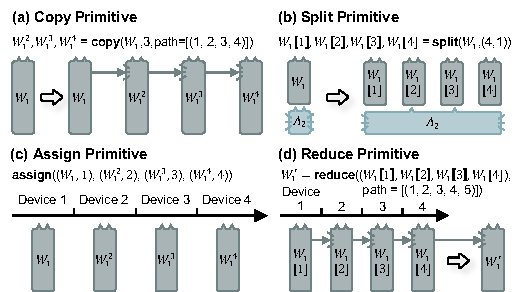
\includegraphics[width=1\linewidth]{figures/primitive_intro1.pdf}
  \vspace{-1.8em}
  \caption{Illustration of data-centric primitives. (a) The \texttt{copy} primitive replicates tensors, enabling data replication across devices. (b) The \texttt{split} primitive partitions tensors, implicitly defining operator partitioning. (c) The \texttt{assign} primitive assigns tensors to devices, implicitly defining operator placement. (d) The \texttt{reduce} primitive manages data movement.}
    \vspace{-1em}
    \label{fig:primitive_intro1}
\end{figure}

During each layer's computation, it may be necessary to gather sharded weights or gradients from other devices; for example, in ZeRO-3, each device must collect all shards of the weight to compute the current layer's forward and backward passes. This process does not need to be explicitly represented in \name{}, as the backend compiler automatically infers and inserts such data-gathering based on data dependencies and constraints (see \cref{sec:automated}). However, if required, the \texttt{reduce} primitive can be used to explicitly specify data gathering or reduction, as shown in Fig.~\ref{fig:primitive_intro1}(d).

\begin{algorithm}[h]
\caption{Primitive program for vanilla DP and ZeRO-1 to 3. Assume the number of devices is 4.}
\label{alg:fsdp}
\begin{algorithmic}[1]
\STATE \# Vanilla DP space: Replicate weights
\STATE $activation[1$ to $4]$ = \textbf{split}($activation$, 4, dim=BATCH)
\STATE \textbf{assign}($activation[i]$, $device_i$)
\STATE $weight^2$, $weight^3$, $weight^4$ = \textbf{copy}($weight$, 3)
\STATE \textbf{assign}($weight^i$, $device_i$) \# $weight^1$ is $weight$
\STATE \# ZeRO-1 space: Add optimizer states sharding
\STATE $opt\_state[1$ to $4]$ = \textbf{split}($opt\_state$, 4)
\STATE \textbf{assign}($opt\_state[i]$, $device_i$)
\STATE \# ZeRO-2 space: Add weight gradients sharding
\STATE $gradient[1$ to $4]$ = \textbf{split}($gradient$, 4)
\STATE \textbf{assign}($gradient[i]$, $device_i$)
\STATE \# ZeRO-3 space: Add weights sharding, no weight copy
\STATE $weight[1$ to $4]$ = \textbf{split}($weight$, 4)
\STATE \textbf{assign}($weight[i]$, $device_i$) 
\STATE \# Explicit all-gather
\STATE $weight\_buf[i]$ = \textbf{reduce}($W[j$ for $j \neq i]$)
\end{algorithmic}
\end{algorithm}



\vspace{-1em}
\subsection{Dependency and Partial Temporal Order}
\label{sec:dependency}

In \cref{sec:primitives_glance}, we demonstrated how \name{} expresses parallelism paradigms (e.g., ZeRO-1 to 3) that are cumbersome to capture with operator-centric primitives. Here, we further illustrate how the data-monistic view articulates new parallelism paradigms. As an example, we can further augment ZeRO-3 with additional constraints: during the backward pass, activations are consumed progressively. The memory released by discarded activations can be immediately reused to host the incoming weight shards of the current layer. By the end of each gradient accumulation step, the model weights are already gathered, thereby eliminating all-gather communication during forward. In the subsequent forward pass, weight shards are discarded layer-by-layer, and the freed space is reclaimed by newly generated activations (ZeRO-3.5).

To implement this, we introduce a new primitive, \texttt{order}. As the event vector of a CAT defines its space-time trajectory (~\cref{sec:abstraction}), the ordering of events governs their temporal execution. A typical use of ordering is to enforce inter-CAT dependencies (Fig.~\ref{fig:abstractions}) or temporal relationships. Consider two CATs, $T_1$ and $T_2$, where $T_2$ can be created only when $T_1$ exists. This translates to the constraint that the start event of $T_2$ ($T_2\rightarrow\mathrm{start}$) occurs before the last event of $T_1$ ($T_1\rightarrow\mathrm{complete}$). We use $T\{i\}$ to reference the $i$-th event in the constraint vector of $T$ ($T\{0\}$ for $T\rightarrow\mathrm{start}$, $T\{-1\}$ for $T\rightarrow\mathrm{complete}$). While the system already preserves dependencies inherited from the original computational graph, the primitive \texttt{order(event$_1$,event$_2$)} explicitly injects additional ordering, ensuring that \texttt{event$_1$} occurs before \texttt{event$_2$}. For ZeRO-3.5, we use \texttt{order($A[i]^{\mathrm{ms}+1}\{-1\}$,$weight\_buf[i]^\mathrm{ms}\{-1\}$)} ($ms$ for micro-batch) to guarantee that weights gathered during backward are retained until the corresponding activations of the next forward are completed. 

\texttt{redirect(tensor$_1$, tensor$_2$, tensor$_3$)} is a syntactic-sugar primitive provided by \name{} for complex dependency operations. For example, if the original dependencies are $T_3 \to T_2 \to T_1$, applying \texttt{redirect(}$T_2, T_4, T_3$\texttt{)} creates a new tensor $T_4$ from $T_2$ ($T_4$ also depends on $T_1$) and changes the dependency of $T_3$ from $T_2$ to $T_4$. The redirect primitive can be used to achieve advanced strategies such as recomputation.
% or asynchronous training plans.



\vspace{-.5em}
\subsection{Parallelism Space Delineation}
\vspace{-.5em}
\label{sec:delineation}

Based on the preceding analysis, \name{}'s primitives are, at their core, a set of declarative constraints. By default, \name{} posits that the initial parallelism space (before any primitives are written) is the universal set of all valid parallelism plans for a given computation graph and hardware system, constrained only by inherent data dependencies. In contrast to existing frameworks, which imperatively construct a plan from a null state, applying a primitive in \name{} is a subtractive process. Each primitive declaratively refines the parallelism search space by imposing an additional constraint, thereby narrowing the universe of valid plans. For example, if Algorithm~\ref{alg:fsdp} is specified only at line 7, the behavior of weight gradients remains unspecified. The strategy space of ZeRO-1 is actually includes ZeRO-2; similarly, the strategy space of ZeRO-3 includes ZeRO-3.5. This approach can yield unforeseen parallelism plans that are not explicitly encoded by the user. The resulting space is then passed to a search algorithm (\cref{sec:search}) and a compilation process (\cref{sec:automated}) to materialize a concrete plan. This design philosophy necessitates that \name{} provide users with mechanisms to guide the delineation of the parallelism plan space and to express design preferences.

\begin{figure}[t]
  \centering
  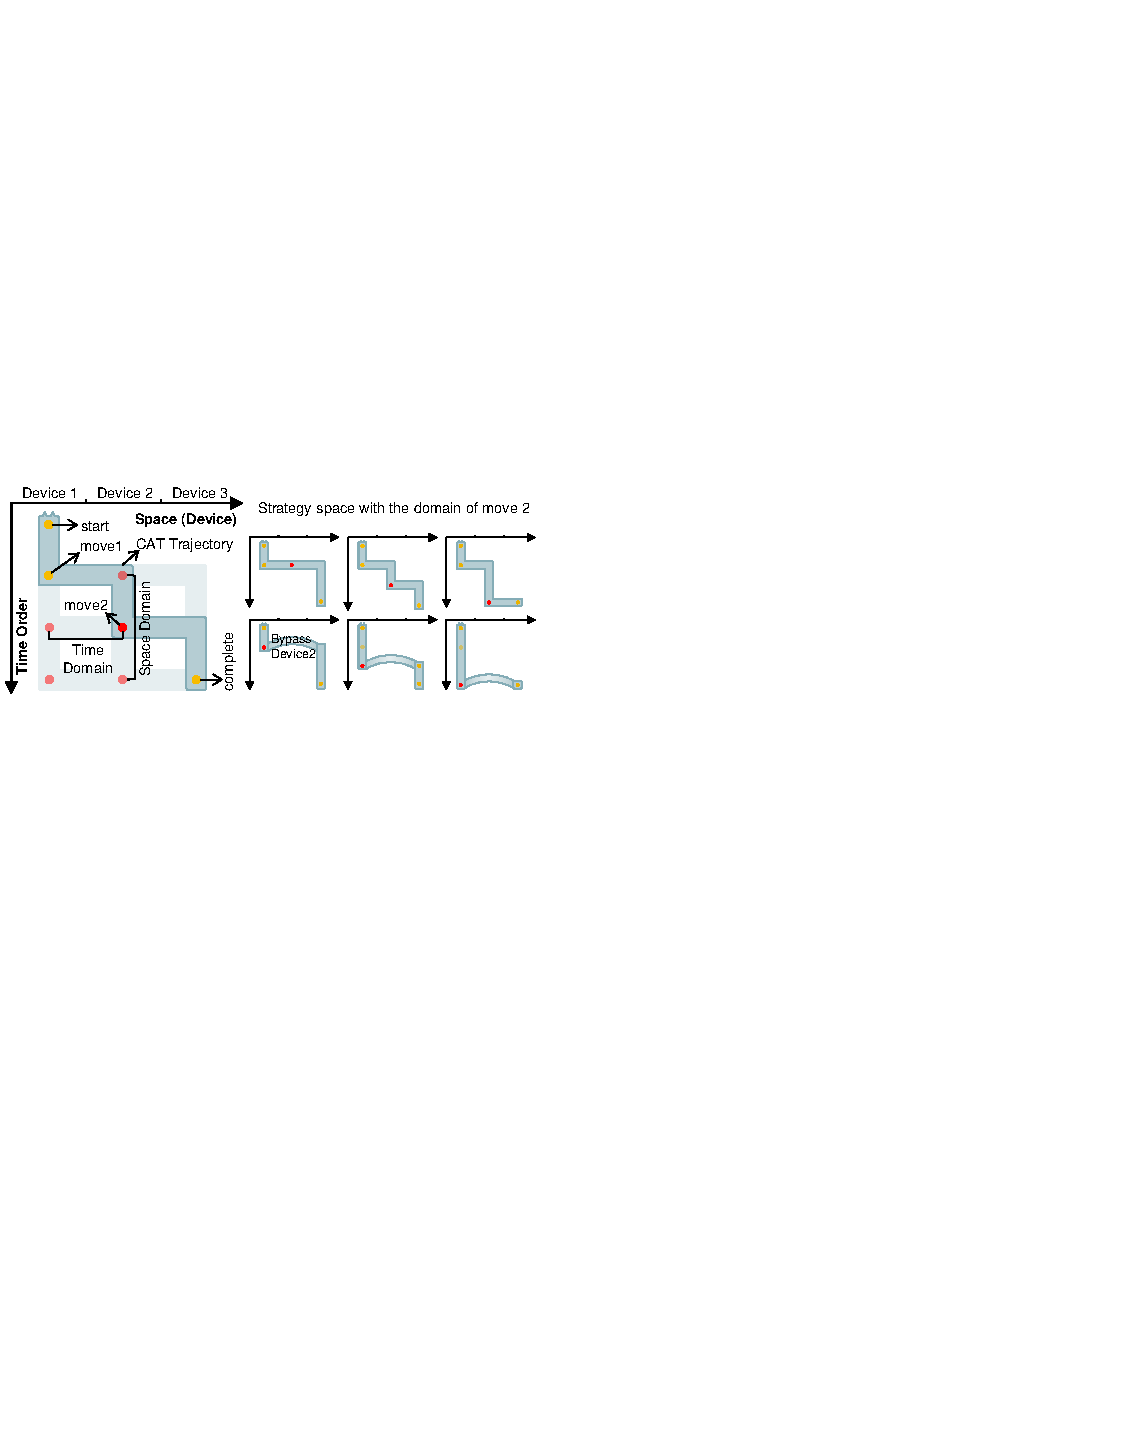
\includegraphics[width=1\linewidth]{figures/primitive_intro2.pdf}
  \vspace{-1.5em}
  \caption{The spatial and temporal domain of \texttt{move2} yields a search space encompassing six feasible CAT trajectories.}
  \vspace{-1.5em}
  \label{fig:primitive_intro2}
\end{figure}

A primary mechanism is the \textbf{\texttt{domain}}. A domain represents a discrete, iterable set of valid candidates for a given parameter, such as a device location or a time step. For example, a user can define \texttt{d=Domain(Device1,Device2,Device3)} and then apply the constraint \texttt{assign(tensor/event,d)}. This declaration constrains the search space by asserting that the assignment must be one of the devices within domain \texttt{d}. As illustrated in Fig.~\ref{fig:primitive_intro2}, imposing event \texttt{move2} in the spatial and temporal domain can yield six possible CAT trajectories in this space. The \textbf{\texttt{not}} declaration allows users to explicitly forbid certain configurations by combining it with the primitives and \texttt{domain}. For instance, \texttt{not(assign(tensor,d))} means the tensor should not be mapped to domain \texttt{d}. The \textbf{\texttt{symmetry}} binds a set of CATs to perform uniform actions during search, reducing search dimensionality and avoiding irregular outcomes. During search, grouped CATs are treated as a single object for move selection and evaluation.




% This biases the search toward coherent patterns while still admitting per-CAT variation via indexed parameters.


% (The temporal domain is a partial-order domain defined by Order Ideals and Order Filters; we do not delve deeper into this topic in the paper.)

% We further introduce \textbf{\texttt{symmetry}}, a mechanism that binds a set of CATs to perform uniform actions during search, thereby reducing search dimensionality and avoiding highly irregular outcomes. Let $S=\{\text{CAT}_1,\ldots,\text{CAT}_k\}$ be a symmetry group and $I=\{1,\ldots,k\}$ its index set. A symmetry declaration is written as \texttt{symmetry($S$,${i\in I \to \mu(i))}$}, where $\mu(i)$ is a parameterized step schema (e.g., \texttt{assign($\text{CAT}_i$,$\text{device}_{\mu(i)}$)}, \texttt{order($\text{CAT}_i$,$W[\mu(i)]$)}). During search, the grouped CATs are treated as a single object for search move selection and evaluation: the algorithm either applies the candidate move to all members simultaneously or to none, and feasibility is jointly assessed across all member constraints. Symmetry-binding thus biases the search toward coherent patterns while still admitting per-CAT variation via indexed parameters. We present more examples of using \name{}'s primitives in Appendix.
\vspace{-.5em}
\section{Parallelism Plan Discovery}

\subsection{Constraint-Based Potential Descent Search}
\label{sec:search}

The fine-grained control over tensor trajectories and the subtractive method of carving the strategy space can result in a potentially larger search space. While this is advantageous for including emergent strategies and creating a more connected, higher-resolution landscape for heuristic search, it also inherently increases the search complexity. Therefore, a biased reduction of the space at the primitive stage is not only necessary but also plays a crucial role in guiding the search. We do not claim that our method can automatically find an optimal strategy from the universal set of all possibilities. Moreover, a rigorous mathematical analysis of the properties of this data-monistic search space, for instance, whether this unified abstraction enhances the topology smoothness and continuity, is beyond the scope of this paper. Instead, this section presents a feasible search algorithm from the CAT perspective. The efficacy of this algorithm in discovering novel strategies will then be demonstrated empirically in Section \ref{sec:exp}.

The search algorithm is inspired by potential-field methods~\cite{koren1991potential}. It reframes the combinatorial-optimization problem as the search for a minimum-energy state in a potential field. At its core, we assigns a potential function to every CAT; each CAT then greedily migrates or transforms to a state that lowers its own potential. A simple illustrative example: suppose CAT1 currently resides on device 1. If we define the potential of CAT1 as the memory already occupied on that device, CAT1 will tend to migrate to a device with lower occupancy (more free memory). Repeating this greedy minimization for every CAT yields a reasonably balanced memory distribution.

% 势能是分层次的，event点处的势能，CAT的整体的势能。核心的点就是是CAT尽量少占用资源。
Real scenarios are far more complicated. A strategy comprises many CATs, and each CAT contains a constraint vector composed of multiple events. Although each event can be scheduled independently, intricate dependencies may exist among events. Our search algorithm therefore employs a two-level potential definition, with each level paired with its own set of searchable actions (the next search move).

Level-1 potential is attached to individual events. In a concrete plan an event’s space–time coordinate is fixed; its potential is therefore quantified by the resource pressure of the underlying hardware at that coordinate. For event $E$:
\begin{equation}\label{eq:event_potential}
P(E) \;=\; \alpha\,\frac{d_c(E)}{C - U_c} \;+\; \beta\,\frac{d_m(E)}{M - U_m} \;+\; \gamma\,\frac{d_b(E)}{B - U_b}
\end{equation}
where $d_c(E)$, $d_m(E)$, and $d_b(E)$ denote the event’s demand on compute, memory, and bandwidth respectively; $C$, $M$, and $B$ are the device capacities; $U_c$, $U_m$, and $U_b$ are the instantaneous usages by other events on the same device; and $\alpha$, $\beta$, $\gamma$ are scalar coefficients. Users can customize the potential function to reflect the optimization objective; for example, when high storage utilization is not the target, the memory‑pressure can be set to zero whenever no overflow occurs.

\begin{algorithm}[t]
\caption{Two-Level Potential-Decent Search Algorithm}
\label{alg:structured_search}
\begin{algorithmic}[1]
\STATE $S \gets S_{initial}$
\FOR{$i = 1$ to $max\_iterations$}
  \STATE $best\_cat \gets \text{None}$; $best\_move \gets \text{None}$; $best\_\Delta \gets 0$
  \FOR{each CAT $T$ in $S$}
    \STATE $P_T \gets \text{CalculateCatPotential}(T, S)$
    \STATE $C_{event} \gets \text{GenerateEventCandidates}(T, S)$
    \STATE $C_{vector} \gets \text{GenerateVectorCandidates}(T, S)$
    \STATE $C_{macro} \gets \text{GenerateMacroCandidates}(T, S)$
    \STATE $M_T \gets C_{event} \cup C_{vector} \cup C_{macro}$
    \STATE $\begin{aligned}
    m_T^{\star} &\gets \operatorname*{argmax}\limits_{m \in M_T} \left(P_T - \text{CalculateCatPotential}(T, \\
    &\text{ApplyCatMove}(S, T, m))\right)
    \end{aligned}$
    \STATE $\begin{aligned}
    \Delta_T &\gets P_T - \text{CalculateCatPotential}(T, \\
    &\text{ApplyCatMove}(S, T, m_T^{\star}))
    \end{aligned}$
    \IF{$\Delta_T > best\_\Delta$}
      \STATE $best\_cat \gets T$; $best\_move \gets m_T^{\star}$; $best\_\Delta \gets \Delta_T$
    \ENDIF
  \ENDFOR
  \IF{$best\_\Delta \le 0$}
    \STATE \textbf{break}
  \ENDIF
  \STATE $S \gets \text{ApplyCatMove}(S, best\_cat, best\_move)$
\ENDFOR
\STATE \textbf{return} $S$
\end{algorithmic}
\end{algorithm}

Level-2 potential is associated with an individual CAT and comprises three components: intrinsic, corrective, and attractive. The intrinsic term sums the event-level potentials in the CAT’s constraint vector $C=(E_1,E_2,\ldots ,E_n)$. The corrective term adds the aggregate potential of events belonging to other CATs coupled via inter-CAT constraints. The attractive term favors retaining a CAT on a device when future CATs on the same device depend on data derived from it. This design provides global awareness without simulating end-to-end performance at every action step. For CAT $T$:
\begin{equation}\label{eq:cat_potential}
P(T)=\sum_{i=1}^{n}P(E_i)+\sum_{T'\in\mathcal{A}(T)}\sum_{j=1}^{m}P(E'_j)+\delta\,A_{\mathrm{attr}}(T)
\end{equation}
where $\sum P(E_i)$ is the $T$'s intrinsic potential, $\mathcal{A}(T)$ is the set of all CATs associated with $T$ via inter-CAT constraints, and $A_{\mathrm{attr}}(T)$ is computed by summing, over future CATs on the same device that depend on data sharing the original identifier with $T$, the positive gap between each dependent’s start time and this $T$’s end time. 


\begin{algorithm}[t]
\caption{GenerateEventCandidates$(T, S)$}
\label{alg:generate_event_candidates}
\begin{algorithmic}[1]
\STATE $C \gets \emptyset$
\FOR{each event $e$ in the constraint vector of $T$}
  \STATE $\mathcal{D}_e \gets \text{AdjacentDevices}(e, S)$
  \STATE $\mathcal{T}_e \gets \text{AdjacentTimes}(e, S)$
  \STATE $m^{st}_e \gets \operatorname*{argmin}\limits_{(d,t) \in \mathcal{D}_e \times \mathcal{T}_e}(\text{EventPotential}(e, d, t, S))$
  \IF{$\text{DecreasePotential}(e, m^{st}_e, S)$ \textbf{and} $\text{Feasible}(e, m^{st}_e, S)$}
    \STATE $C \gets C \cup \{\text{MakeMove}(e, m^{st}_e)\}$
  \ENDIF
\ENDFOR
\STATE \textbf{return} $C$
\end{algorithmic}
\end{algorithm}


\begin{figure*}[h]
  \centering
  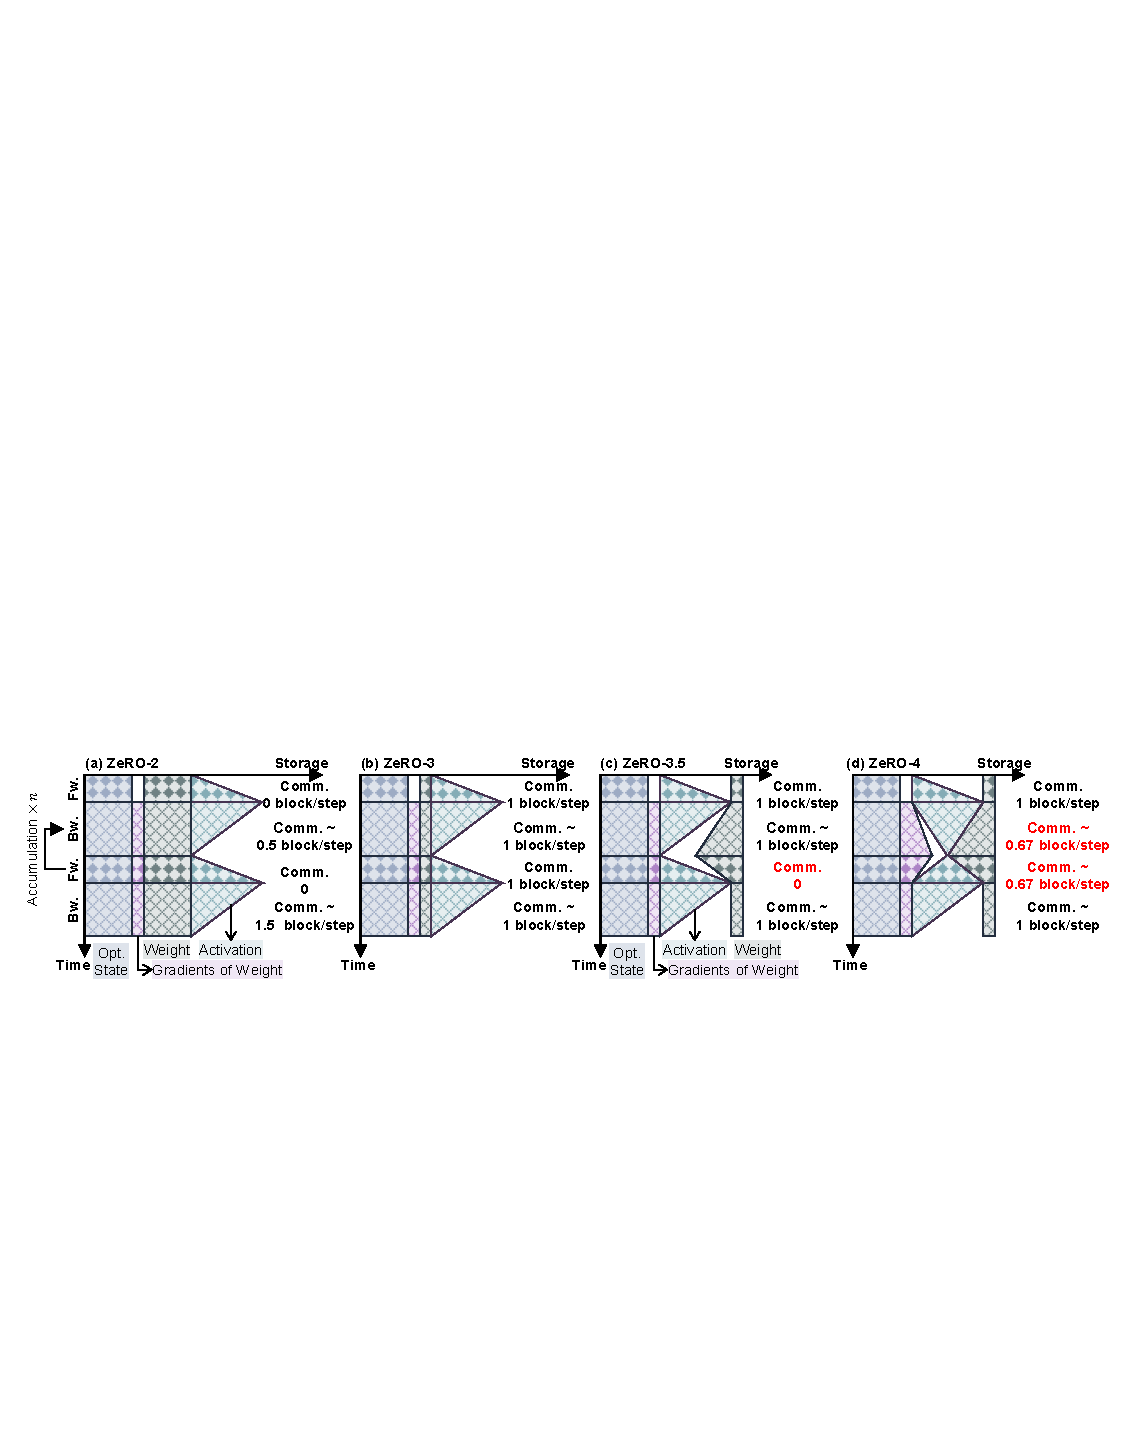
\includegraphics[width=1\linewidth]{figures/FSDP.pdf}
  \vspace{-2em}
  \caption{Memory and averaged communication over time for ZeRO-2, 3, 3.5, and 4. Assume each layer's forward computation takes 1 time step and each device transmits 1 block of data per weight or gradient transfer. The backward takes 2 time steps. Details for calculating averaged communication over time are omitted for simplicity.}
  \vspace{-1em}
  \label{fig:FSDP}
\end{figure*}


Search actions for a CAT fall into three categories: (1) modify a single event in the constraint vector—moves are atomic to handle inter-event constraints, and the best change follows the steepest descent of the event’s Level-1 potential (\texttt{GenerateEventCandidates}); (2) change the vector’s dimensionality by deleting an event or inserting a event in the tensor trajectory (\texttt{GenerateVectorCandidates}); (3) apply macro scheduling to the whole CAT (split, copy, reduce) (\texttt{GenerateMacroCandidates}). Available transformations are enumerated from permitted high-level policies. The union of these categories forms the candidate set for the CAT’s next move. The search is greedy and iterative. Starting from an initial strategy sampled from the space, each iteration computes every CAT’s potential, finds its best next move (maximum potential drop), then globally selects the CAT with the largest drop and commits its move. The process repeats until the stop condition. Algorithm~\ref{alg:structured_search} instantiates the potential-descent search.



Algorithm~\ref{alg:generate_event_candidates} shows the detailed routine of \texttt{GenerateEventCandidates}. Device candidates are enumerated from the spatial adjacents; time candidates are the immediately preceding or succeeding order positions. For each event, the routine enumerates the Cartesian product of adjacent devices and times, evaluates the event potential on each spatiotemporal pair, and selects the steepest-descent pair while preserving all constraints.

\subsection{Representative Newly Discovered Plans}

In this section, we introduce two representative strategies discovered automatically by \name{}, ZeRO-3.5 \& 4 (detailed search analysis in \cref{sec:exp_search}). Compared to ZeRO-3 that shards weights throughout training and therefore requires all-gather in both forward and backward passes to assemble full weights, ZeRO-3.5 does not reshard the gathered weights during the backward pass. Instead, these gathered weights are retained and reused in the next accumulation step's forward pass, eliminating the forward all-gather. As shown in Fig.~\ref{fig:FSDP}(c), during the backward pass, ZeRO-3.5 reclaims memory from progressively released activations and uses it to hold the gathered weight shards; when the total activation memory exceeds the total weight memory, ZeRO-3.5 achieves the same peak memory as ZeRO-3 while removing forward all-gather communication (1 block/step in Fig.~\ref{fig:FSDP}(b)).

Building on ZeRO-3.5, ZeRO-4 further selectively delays reduce-scatter operations on gradients (realized by \texttt{order($A[j]^{\mathrm{microbatch}+1}\{-1\}$,$G[j]^{\mathrm{microbatch}}\{0\}$)} in \name{}). This allows part of gradients to remain on the local device during backward instead of being immediately communicated; the reduce-scatter is postponed to the next forward pass. As shown in Fig.~\ref{fig:FSDP}(d), during backward, activations are progressively released and the freed memory accommodates the gathered weights and the deferred gradients. In the subsequent forward pass, gradients are reduced and weights are discarded to free memory for newly generated activations. In Fig.~\ref{fig:FSDP}(d), we retain two layer's gradients for every three layers (choose $j$ as multiples of three); in practice, $j$ can be tuned according to actual resource usage. ZeRO-4 achieves a more balanced backward-forward communication pattern (0.67 block/step in Fig.~\ref{fig:FSDP}(d)) than ZeRO-3.5, which can benefit from better communication-computation overlap.




\cref{sec:exp} presents further plans discovered by \name{}.

% \begin{table}[h]
% \centering
% \small
% \caption{Average communication volume over time for ZeRO-2, 3, 3.5, 4. Assume each layer's forward computation takes one unit and each device transmits one unit of data per weight or gradient transfer. The duration of backward is two units.}
% \vspace{-0.3em}
% \label{tab:zero}
% \begin{tabular}{lcccc}
% \toprule
% \textbf{Step} & \textbf{ZeRO-2} & \textbf{ZeRO-3} & \textbf{ZeRO-3.5} & \textbf{ZeRO-4} \\
% \midrule
% $1^{st}$ Fw. & 0 & 1 & 1 & 1 \\
% Intermed. Bw. & 0.5 & 1 & 1 & 0.67 \\
% Intermed. Bw. & 0 & 1 & 0 & 0.67 \\
% Last Bw. & 1.5 & 1 & 1 & 1 \\
% \bottomrule
% \end{tabular}
% \end{table}



\vspace{-.5em}
\section{Implementation}
\label{sec:automated}

% because it builds on the explicit scheduling of data trajectories
The data-monistic abstraction of \name{} represents a paradigm shift from existing operator-centric distributed-training frameworks such as DeepSpeed~\cite{rasley2020deepspeed} or Megatron, whose core architectures (IR, schedulers, runtimes) are deeply integrated to schedule operators. Retrofitting \name{} into these frameworks is extremely difficult. Moreover, this architectural mismatch culminates in an incompatible runtime. While existing systems are designed to execute a pre-compiled sequence of computational kernels and communication collectives, it remains an open research topic how to dynamically interpret a data-centric schedule to generate efficient low-level CUDA kernels on the fly. Therefore, \name{} is not implemented as an end-to-end system but rather serves as a strategy-exploration framework. It discovers parallelization plans that are then manually implemented in CUDA kernels or existing frameworks for high-performance execution.

Beyond these difficulties, our implementation focuses on two aspects: (1) Primitive Compilation \& Strategy-Space IR (IR1) — the design of the primitive interface in high-level languages and its compilation into a constraint-declarative strategy-space IR; (2) Search \& Plan Synthesis (IR2) — the search procedure over IR1, augmented with automatic management rules, that yields a concrete parallelization plan. The implementation stack of \name{} is shown in Figure \ref{fig:implementation}.


\begin{figure}[t]
  \centering
  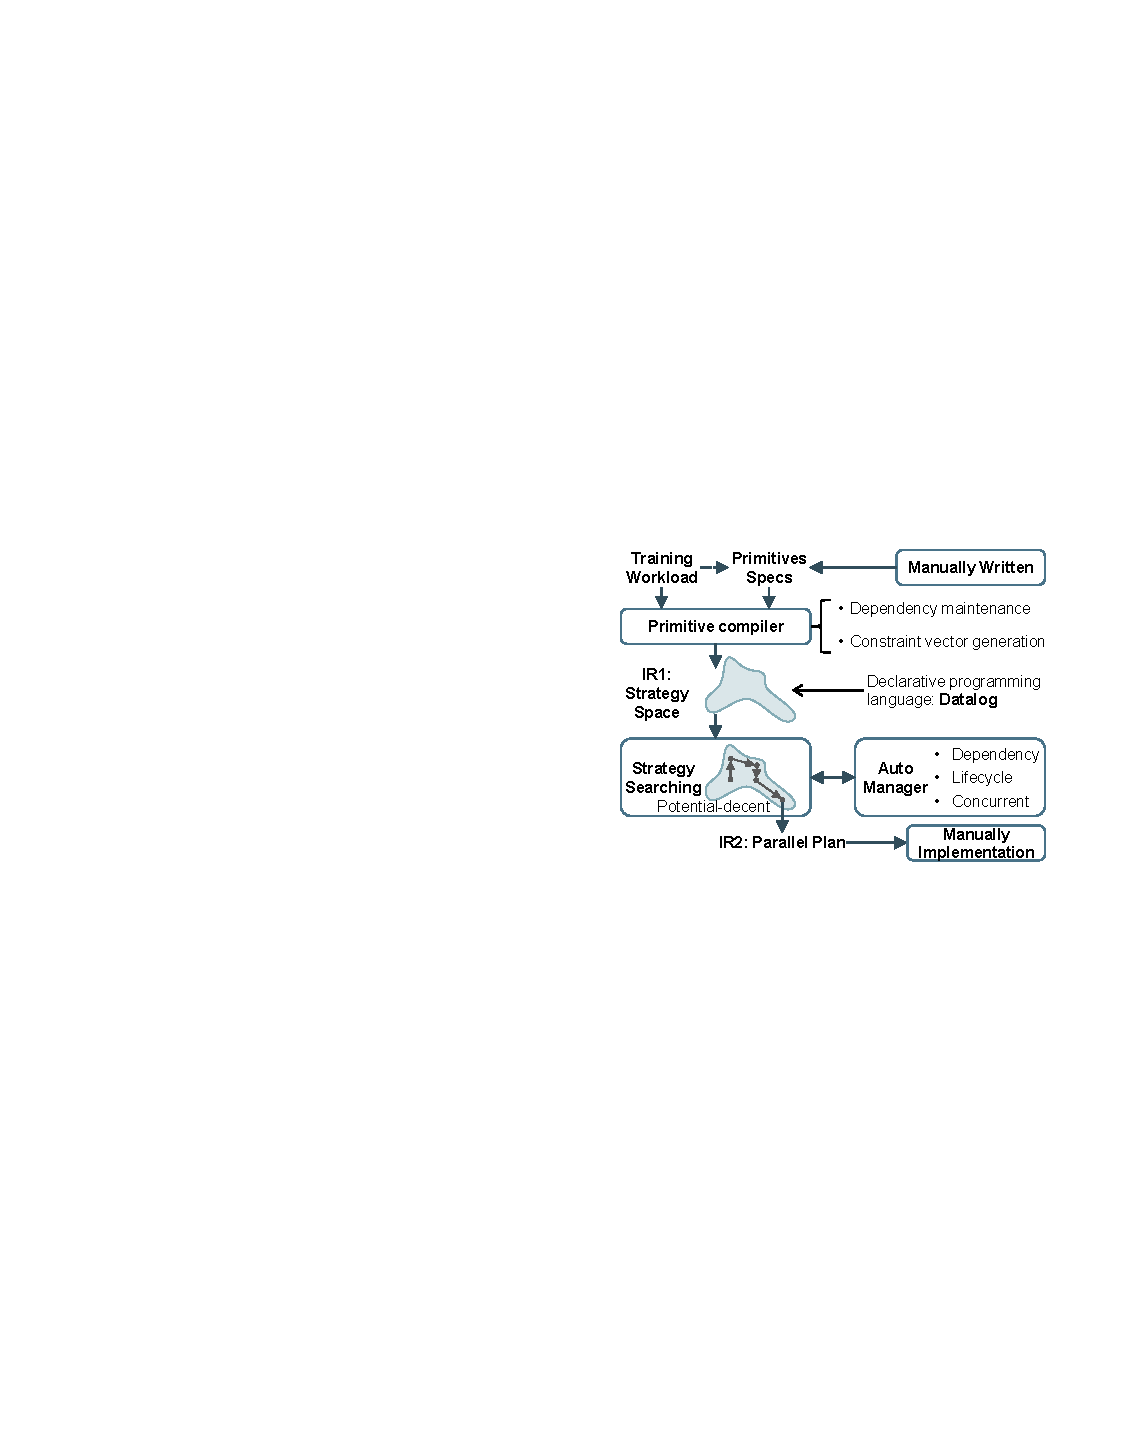
\includegraphics[width=0.7\linewidth]{figures/implementation.pdf}
      \vspace{-.5em}
  \caption{Implementation stack of \name{}.}
    \label{fig:implementation}
    \vspace{-1.5em}
\end{figure}

\subsection{Primitive Compilation}
\label{sec:primitive_compilation}

We implement our primitives in Python, with the tensor identifier coming from the training workload. Each primitive invocation is translated into a set of declarative constraints in Datalog; the strategy-space IR1 itself is represented in Datalog to enable constraint normalization. Datalog is a declarative logic-programming language based on Horn clauses. We adopt Datalog because it is a universal language for constraint specification and integrates cleanly with Python. IR1 captures, for every CAT, its constraint vector (events), the spatial and temporal domains of each event, inter-CAT couplings, and resource constraints. The primitive compiler is responsible for maintaining IR invariants while applying the transformations specified by the primitives. The most critical invariant is dependency preservation: if a CAT $B$ depends on CAT $A$, and a primitive transforms $A$ (e.g., \texttt{split}, \texttt{copy}) into derived CATs or data blocks, the compiler rewrites $B$'s dependencies to target the transformed set that semantically replaces $A$.




To ensure correct dependency rewriting, every data block in the training workload is assigned a globally unique identifier. Derived blocks carry provenance metadata of the form $(\text{origin\_id}, \text{range})$, which records their position within the original tensor. When primitives create new blocks, the compiler compares the positional intervals of producer and consumer blocks: overlaps introduce new dependencies, whereas disjoint intervals allow the dependency to be removed. nnScaler employs a similar mechanism; we therefore adopt its intersection-based matching approach. For \texttt{copy} primitives that may introduce redundant dependencies, the compiler retains the redundancy and defers selection of the optimal dependency to the plan-synthesis stage.

Temporal constraints are encoded through a Lamport logical time system. Each event is assigned a unique timestamp; however, when an event possesses a temporal domain, its timestamp is superseded by a partial-order domain induced by other events. For instance, if event $e$ must occur after both $e_1$ and $e_2$ and before $e_3$, and $e_1$ and $e_2$ are unordered, the constraint is represented as $(\{e_1,e_2\},e_3)$.

Each CAT is associated with a constraint vector for events. The compiler designates the first point of the vector as the generation event of the CAT and the final point as its release event. Intermediate points are interpreted as \emph{move} events, indicating a change in the CAT's spatial location. If such an event does not alter the spatial coordinates, the compiler eliminates it and rewrites any dependencies that involved the removed event to its nearby event.

\subsection{Plan Synthesis}
\label{sec:plan_synthesis}

The strategy search is performed via the potential-descent algorithm described in Section~\ref{sec:search}. At every search iteration, a concrete strategy (IR2) within the space is synthesized. To ensure unambiguous interpretation, we adopt a set of default management rules that complement the explicitly constraints.

\begin{figure}[t]
  \centering
  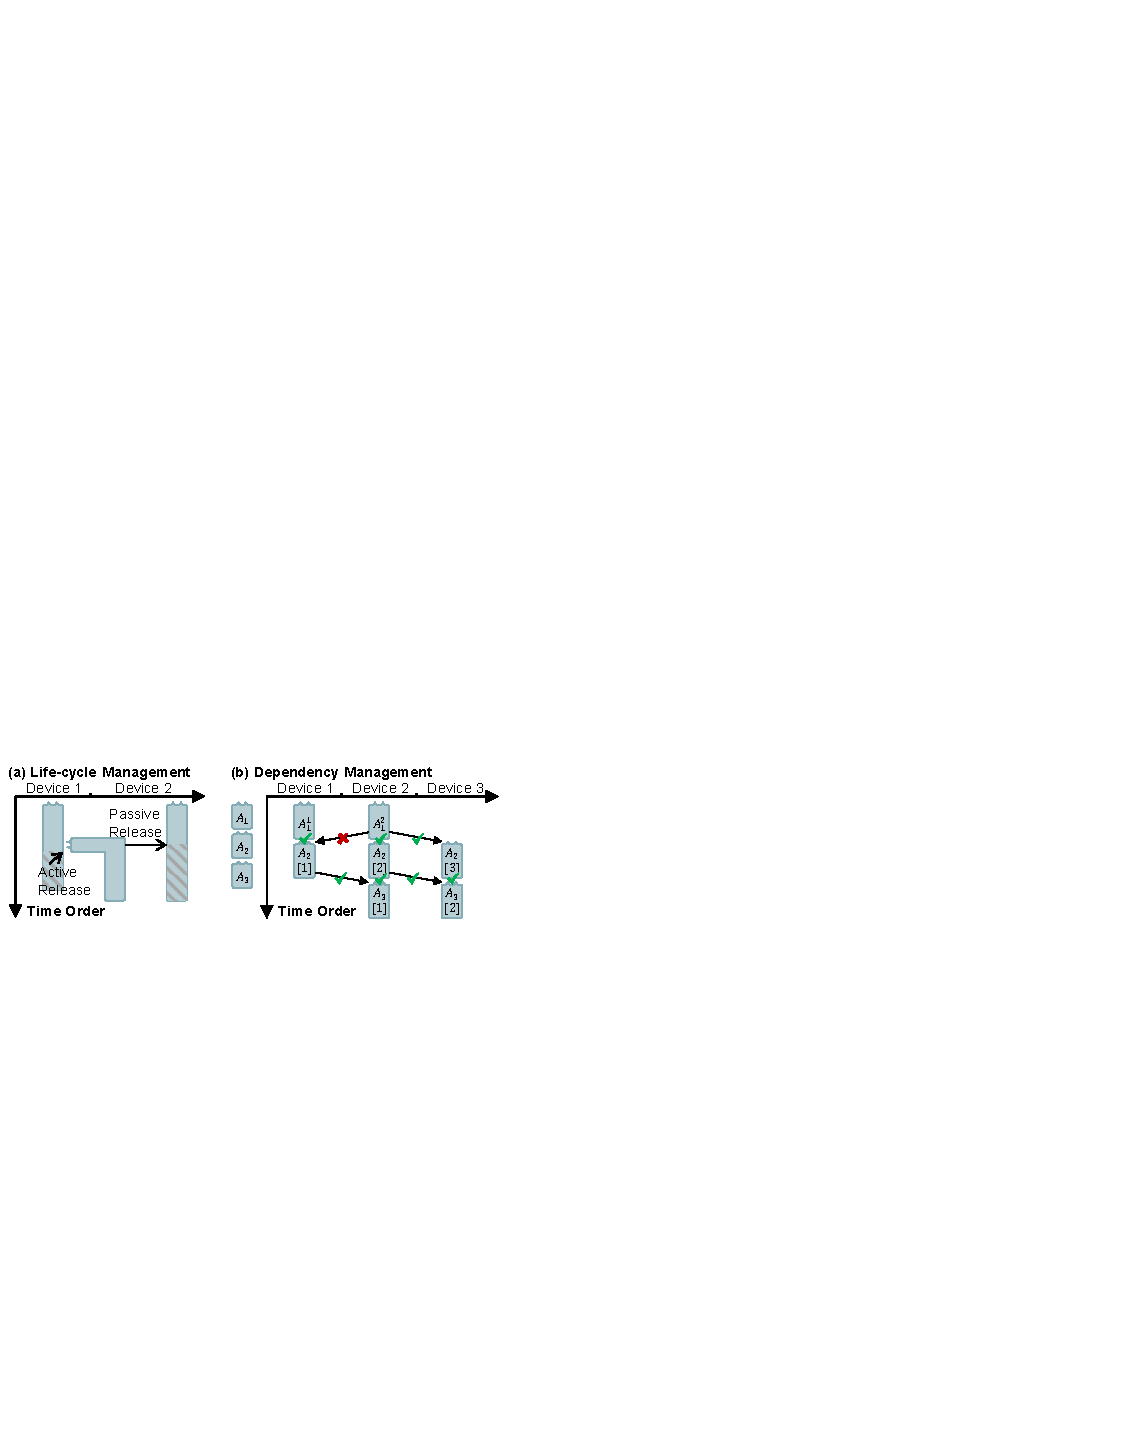
\includegraphics[width=0.95\linewidth]{figures/management.pdf}
  \caption{Example of lifecycle and dependency management.}
  \vspace{-1em}
    \label{fig:management}
\end{figure}

\textbf{Lifecycle Management:} The lifecycle ensures that each tensor is properly released after its usage. It implements two rules: (1) \emph{active release}: a CAT is freed immediately once no subsequent event depends on it; (2) \emph{passive release}: a CAT may remain in memory even when unreferenced, but is evicted when memory pressure exceeds a predefined threshold (Figure~\ref{fig:management}(a)). These rules may steer the search algorithm toward different strategies due to their different influences on potential evaluation.

\textbf{Dependency Management:} A CAT may depend on other CATs whose data are scattered across multiple devices. The \texttt{copy} primitive can also render the dependencies recorded in IR1 redundant. The dependency manager therefore materializes a CAT's complete forward dependencies on demand. It first enumerates every required predecessor, then fetches them in ascending order of estimated acquisition cost until all dependencies are satisfied. For instance, if CAT $A$ on device-1 needs CAT $B$ and $B$ exists on both device-1 and device-2, $A$ prefers to consume the local replica, eliminating inter-device transfer. Figure~\ref{fig:management}(b) illustrates some cases involving \texttt{split} and \texttt{copy}.

\textbf{Concurrent Management:} Events whose temporal order is unspecified may be executed concurrently. We currently model the most common case: overlapping computation with communication. Other concurrent events are temporarily excluded because it is hard to find universal rules for them. For example, multiple move events will still be executed in a default order even when no order constraint is imposed.

\section{Evaluation}
\label{sec:exp}
\subsection{Experiment Setup}
\label{sec:exp_setting}

We structure our evaluation in three phases to assess the efficiency of \name{}'s generated strategies and its search procedure. First, we compare ZeRO-2 and ZeRO-3~\cite{rajbhandari2020zero} to ZeRO-3.5 and ZeRO-4 across different LLMs and hardware configurations, focusing on training throughput and peak memory usage. Second, we demonstrate \name{}'s search capability: starting from a ZeRO-3 initialization, we trace how the potential distribution evolves under potential descent toward ZeRO-3.5 and ZeRO-4. Finally, through comprehensive analysis, we identify seven scheduling optimization directions suggested by potential descent under various hardware resource constraints. By combining several of these directions, \name{} proposes and implements a novel offloading strategy. 

\name{}'s expressiveness and search capability enable the exploration of coordinated, cross-resource trade-offs, including leveraging partial redundancy in one resource to alleviate bottlenecks in another. Accordingly, \name{} focuses on improving utilization with tight resource budgets on small clusters, rather than on scaling under ever-increasing resources. The objective is to democratize the training of LLMs for small companies and laboratories~\cite{sun2025mepipe}. Consistent with this objective, we perform the experiments at scale with 8 GPUs.

\textbf{Models and Hardware.} We evaluate strategies on 8B, 14B, and 32B models (Qwen3 family~\cite{yang2025qwen3}). For hardware, we use four configurations: NVIDIA A100-NVLink, H20-NVLink, H800-PCIe, and A100-PCIe. Compute capacity: H800 > A100 > H20; interconnect bandwidth: H20-NVLink (900 GB/s) > A100-NVLink (400 GB/s) > H800-PCIe (128 GB/s) > A100-PCIe (64 GB/s); memory capacity: H20-NVLink (96 GB) > H800-PCIe = A100-NVLink (80 GB) > A100-PCIe (40 GB). Intel Xeon Platinum 8558 CPU (80/96/128/160 cores) is adopted for offload experiments.

% \begin{table}[t]
%   \centering
%   \caption{Qwen3 series model configurations}
%   \vspace{-0.5em}
%   \label{tab:qwen3_params}
%   \begin{tabular}{ccccc}
%     \toprule
%     Model & Params & Layers & Hidden & Heads (Q/KV) \\
%     \midrule
%     Qwen3  & 8B  & 36 & 4096  & 32/8 \\
%     Qwen3 & 14B & 40 & 5120 & 40/8 \\
%     Qwen3 & 32B & 64 & 5120 & 64/8 \\
%     \bottomrule
%   \end{tabular}
%   \vspace{-1em}
% \end{table}

\textbf{Implementation and Configuration.} For potential evaluation during search, we use a behavioral simulator that estimates compute, storage, and bandwidth usage, calibrated against an A100-based cluster. On real systems, we extend DeepSpeed's ZeRO-3 implementation with ZeRO-3.5/4 and offload-related strategies, and we unify other settings (e.g., reduce/prefetch bucket sizes, maximum live parameters) to ensure fair comparisons. We replace the default Linear layer with a memory-efficient Linear to mitigate potential memory leakage in DeepSpeed.\footnote{\url{https://github.com/deepspeedai/DeepSpeed/issues/3378}.} We use FP16-FP32 mixed-precision training. Detailed configurations are reported with the results. 

% For each strategy, we sweep batch sizes and sequence lengths;



\subsection{Evaluation on New ZeRO Strategies}
\label{sec:exp_zeros}

\subsubsection{Performance and Memory Comparison}
\label{sec:zero_performance}

Fig.~\ref{fig:zero_comparison} compares the performance and memory footprint of ZeRO-2, ZeRO-3, ZeRO-3.5, and ZeRO-4 across different hardware and model settings. These experiments use 8 GPUs, 16 accumulation steps, and micro-batch sizes per device of 1 and 2 (total batch sizes 128 and 256). Results for Qwen3-14B on A100-PCIe (40\,GB) are omitted due to OOM in most configurations. In ZeRO-3.5 (Fig.~\ref{fig:FSDP}(c)), the backward pass reuses activation memory that is progressively released to hold gathered weight shards; the gathered weights are discarded in the subsequent forward step to free space for activations. This preserves ZeRO-3's peak memory (Fig.~\ref{fig:zero_comparison}(f)) while eliminating forward all-gather communication, resulting in up to a 31.6\% throughput improvement over ZeRO-3 (Fig.~\ref{fig:zero_comparison}(c)). ZeRO-4 further retains a portion of unreduced gradient buckets in the freed activation memory and defers their reduce-scatter to the next forward pass (Fig.~\ref{fig:FSDP}(d)). By shifting part of the backward communication into the forward pass and overlapping it with forward computation, ZeRO-4 achieves more balanced communication and up to a 39.1\% throughput improvement.


\begin{figure}[t]
  \centering
  \begin{subfigure}{0.7\linewidth}
    \centering
    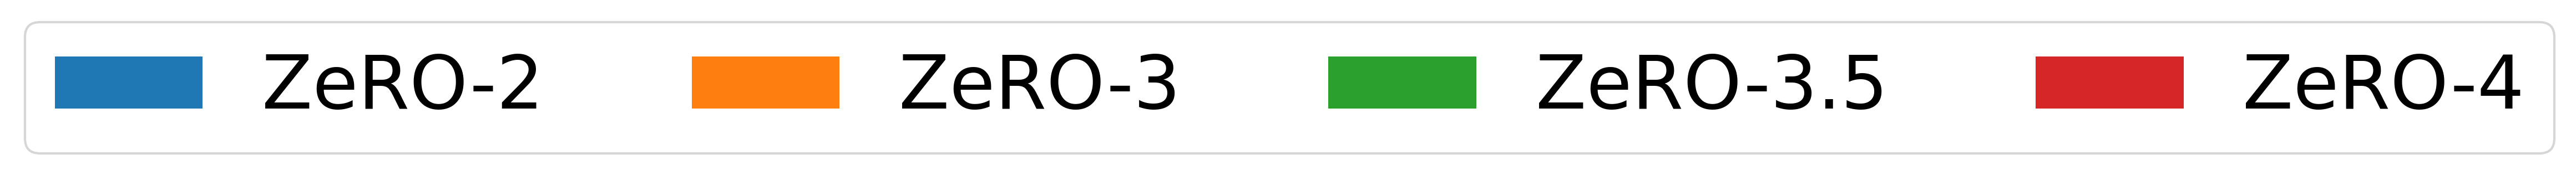
\includegraphics[width=\linewidth]{figures/legend.png}
    \vspace{-1.4em}
  \end{subfigure}
  \begin{subfigure}{0.49\linewidth}
    \centering
    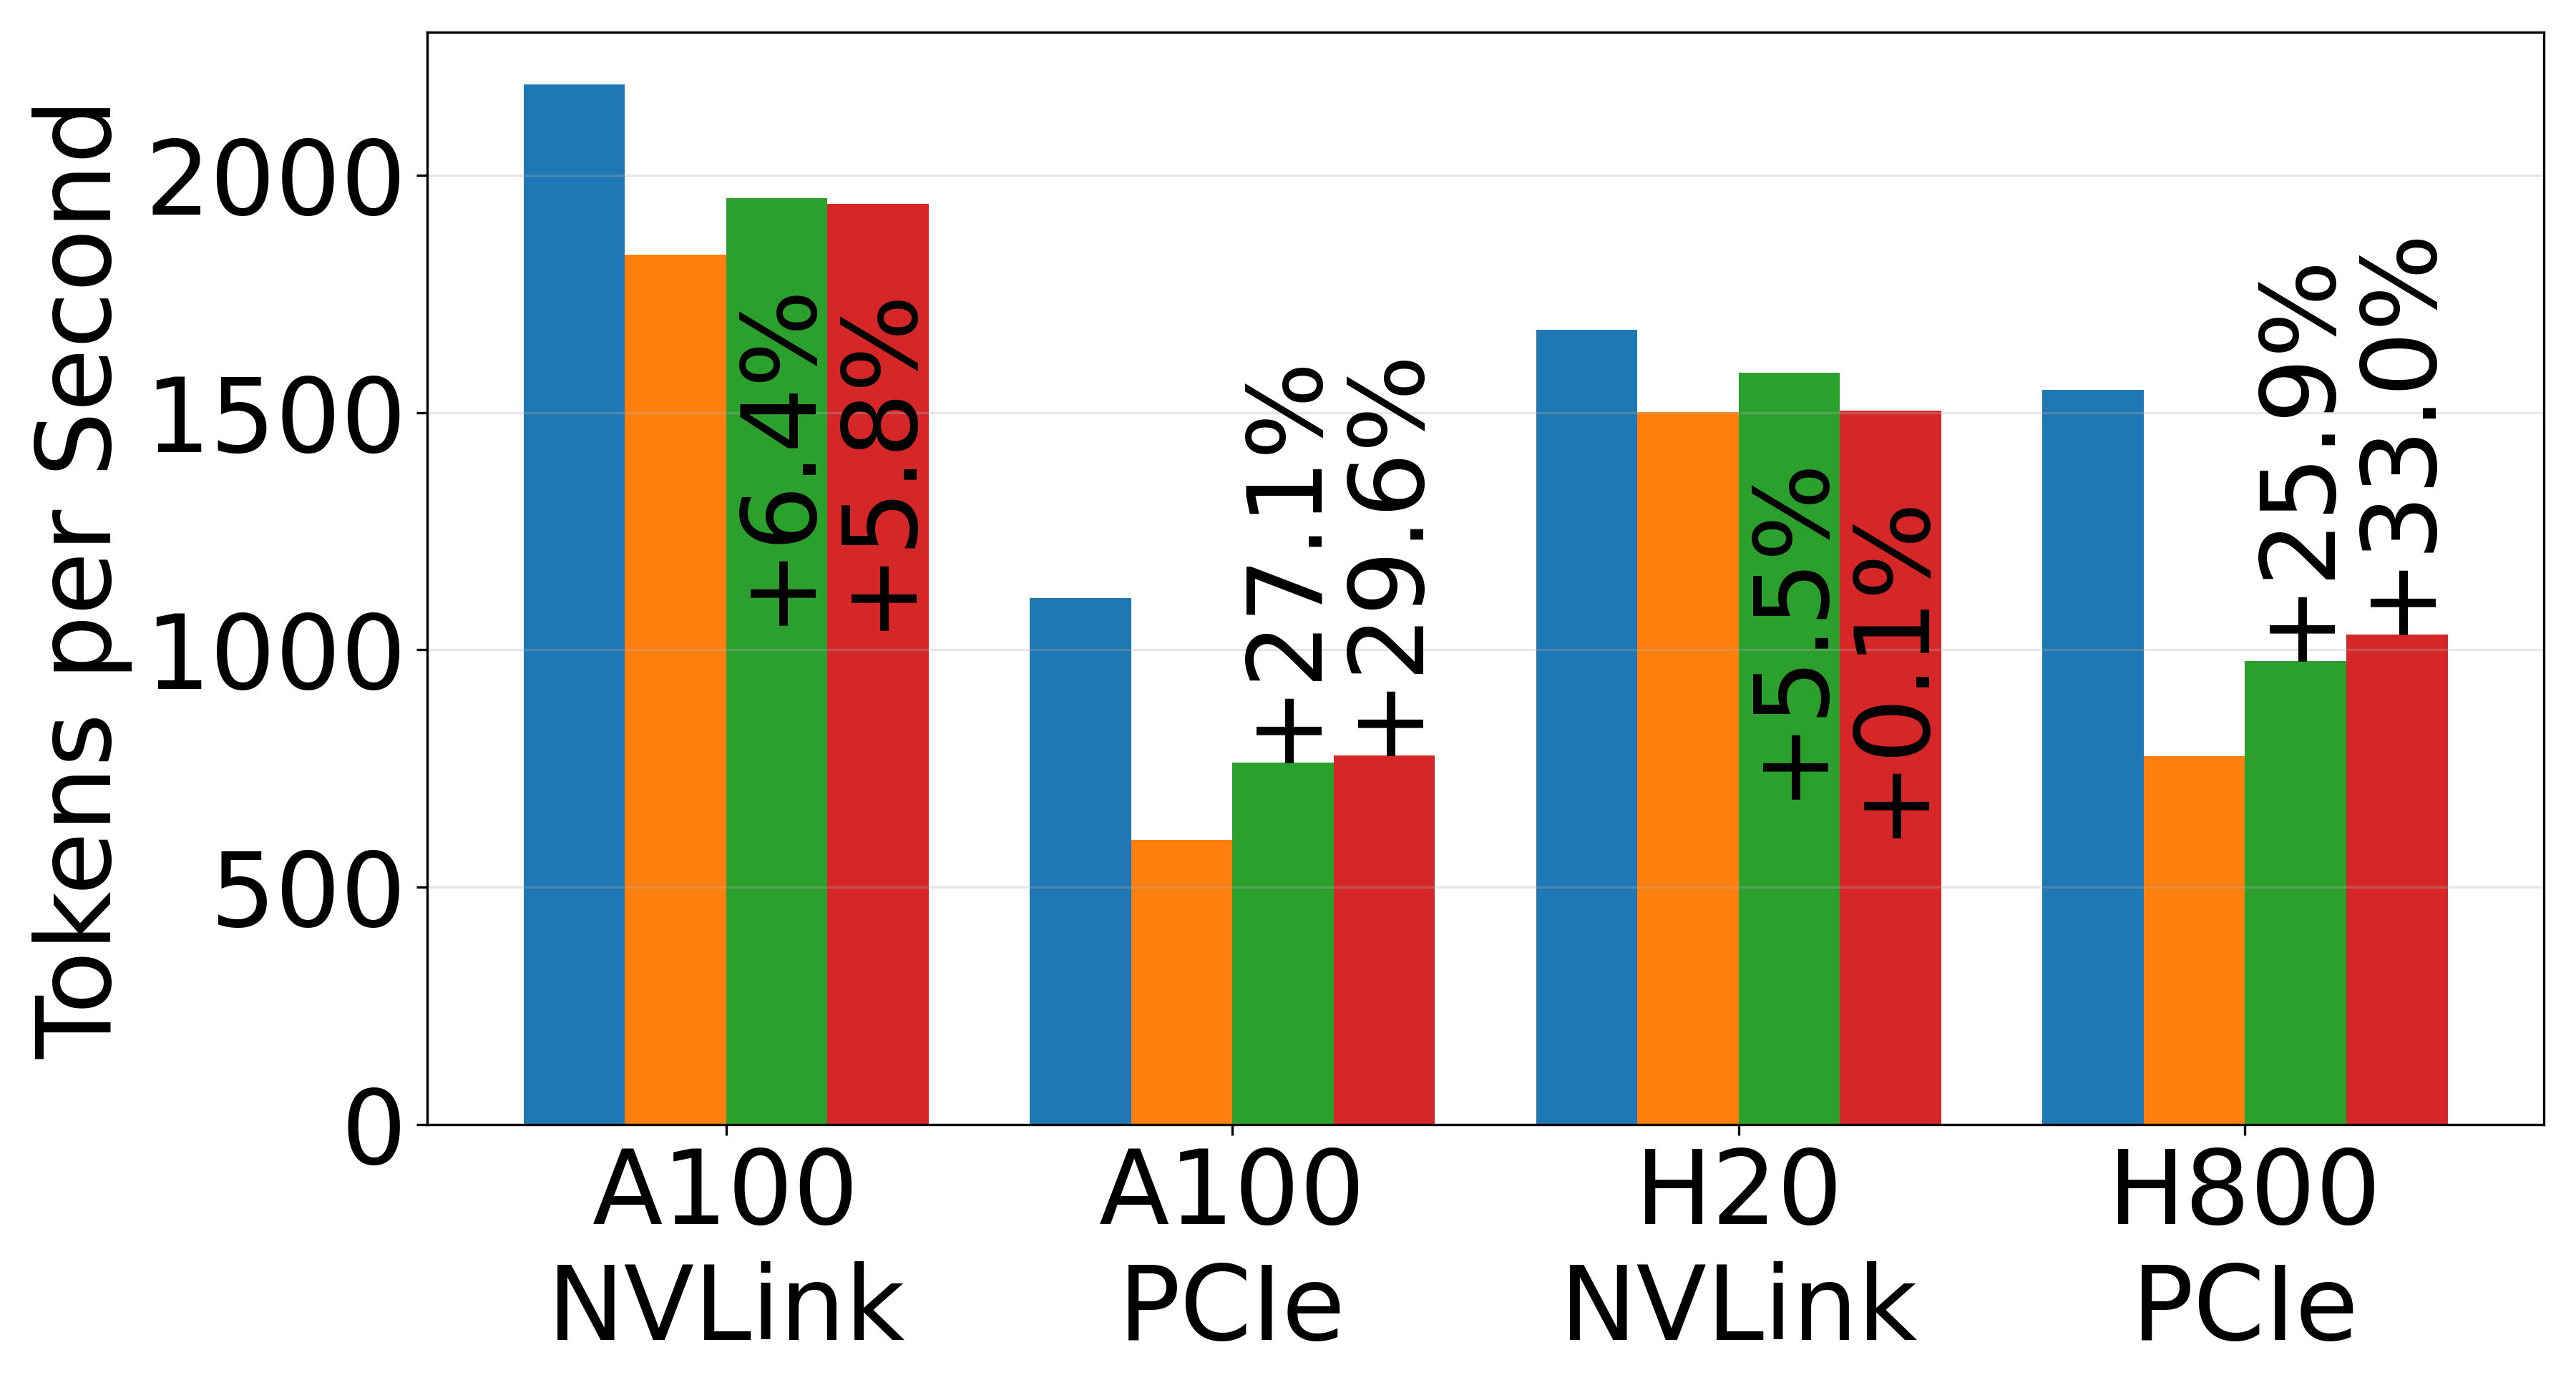
\includegraphics[width=\linewidth]{figures/hardware_comparison_b1_s1536_tokens_per_sec_qwen3-8b.png}
    \vspace{-1.5em}
    \caption{8B|B=128|S=1.5K}
  \end{subfigure}
  \begin{subfigure}{0.49\linewidth}
    \centering
    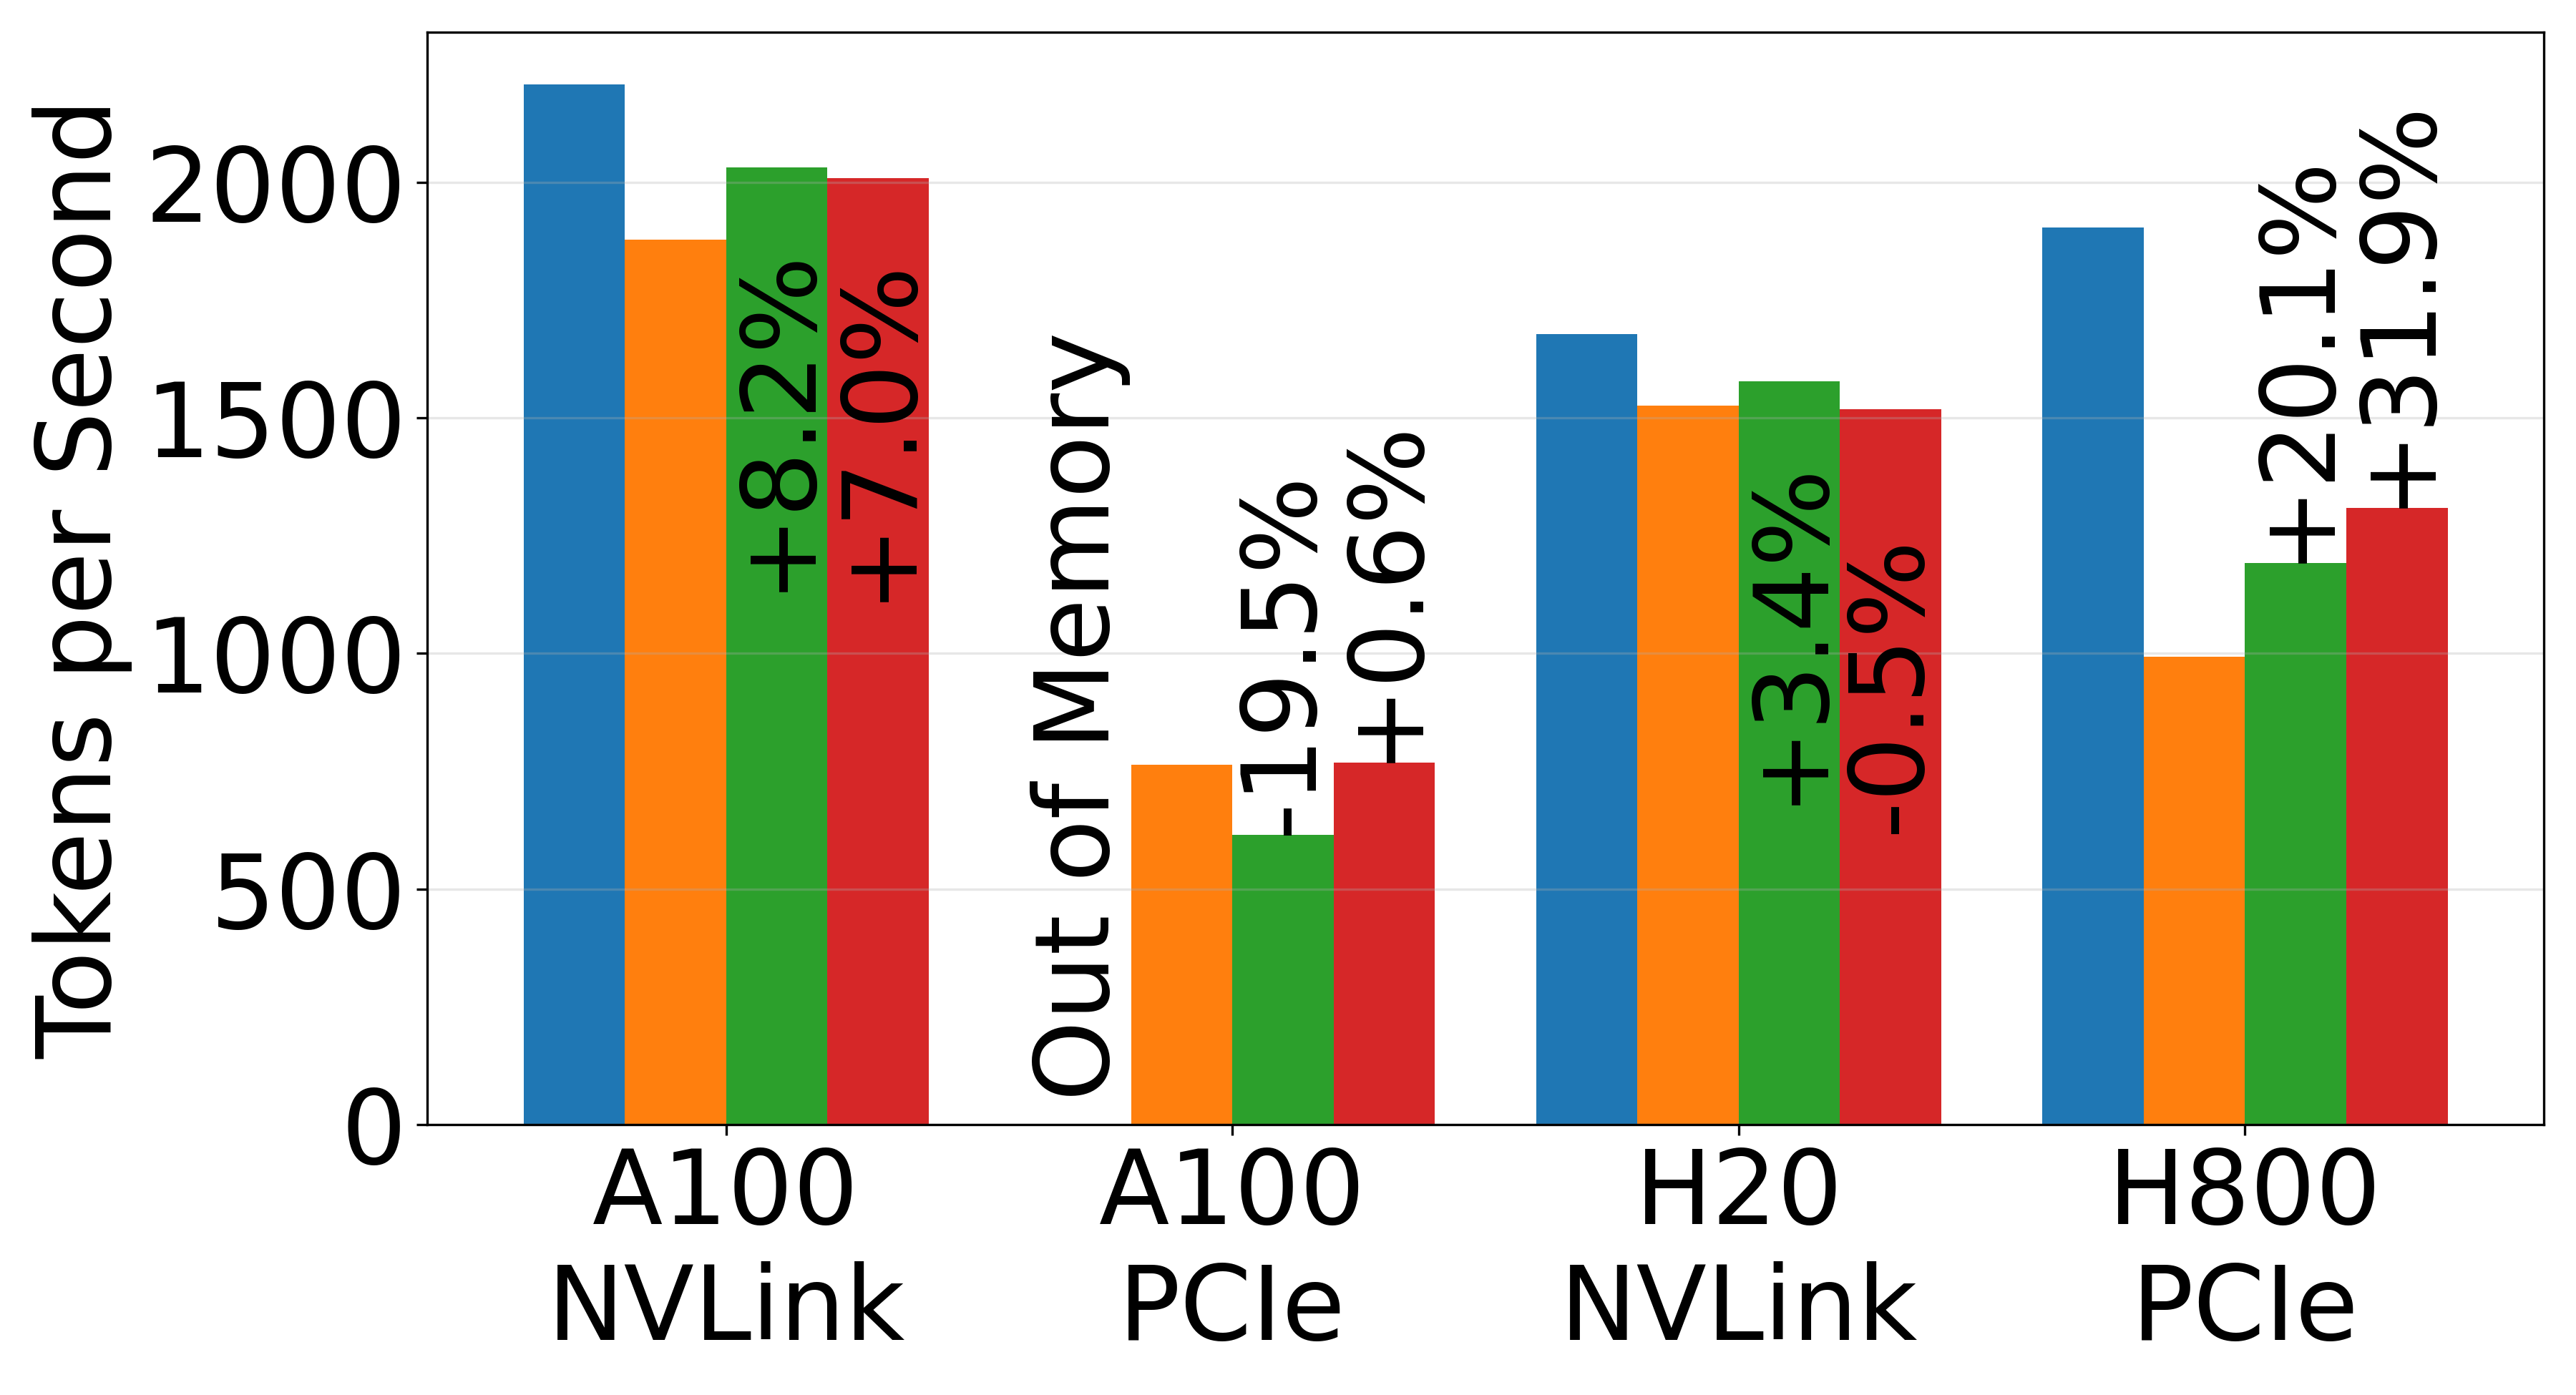
\includegraphics[width=\linewidth]{figures/hardware_comparison_b1_s2048_tokens_per_sec_qwen3-8b.png}
    \vspace{-1.5em}
    \caption{8B|B=128|S=2K}
  \end{subfigure}
  \begin{subfigure}{0.322\linewidth}
    \centering
    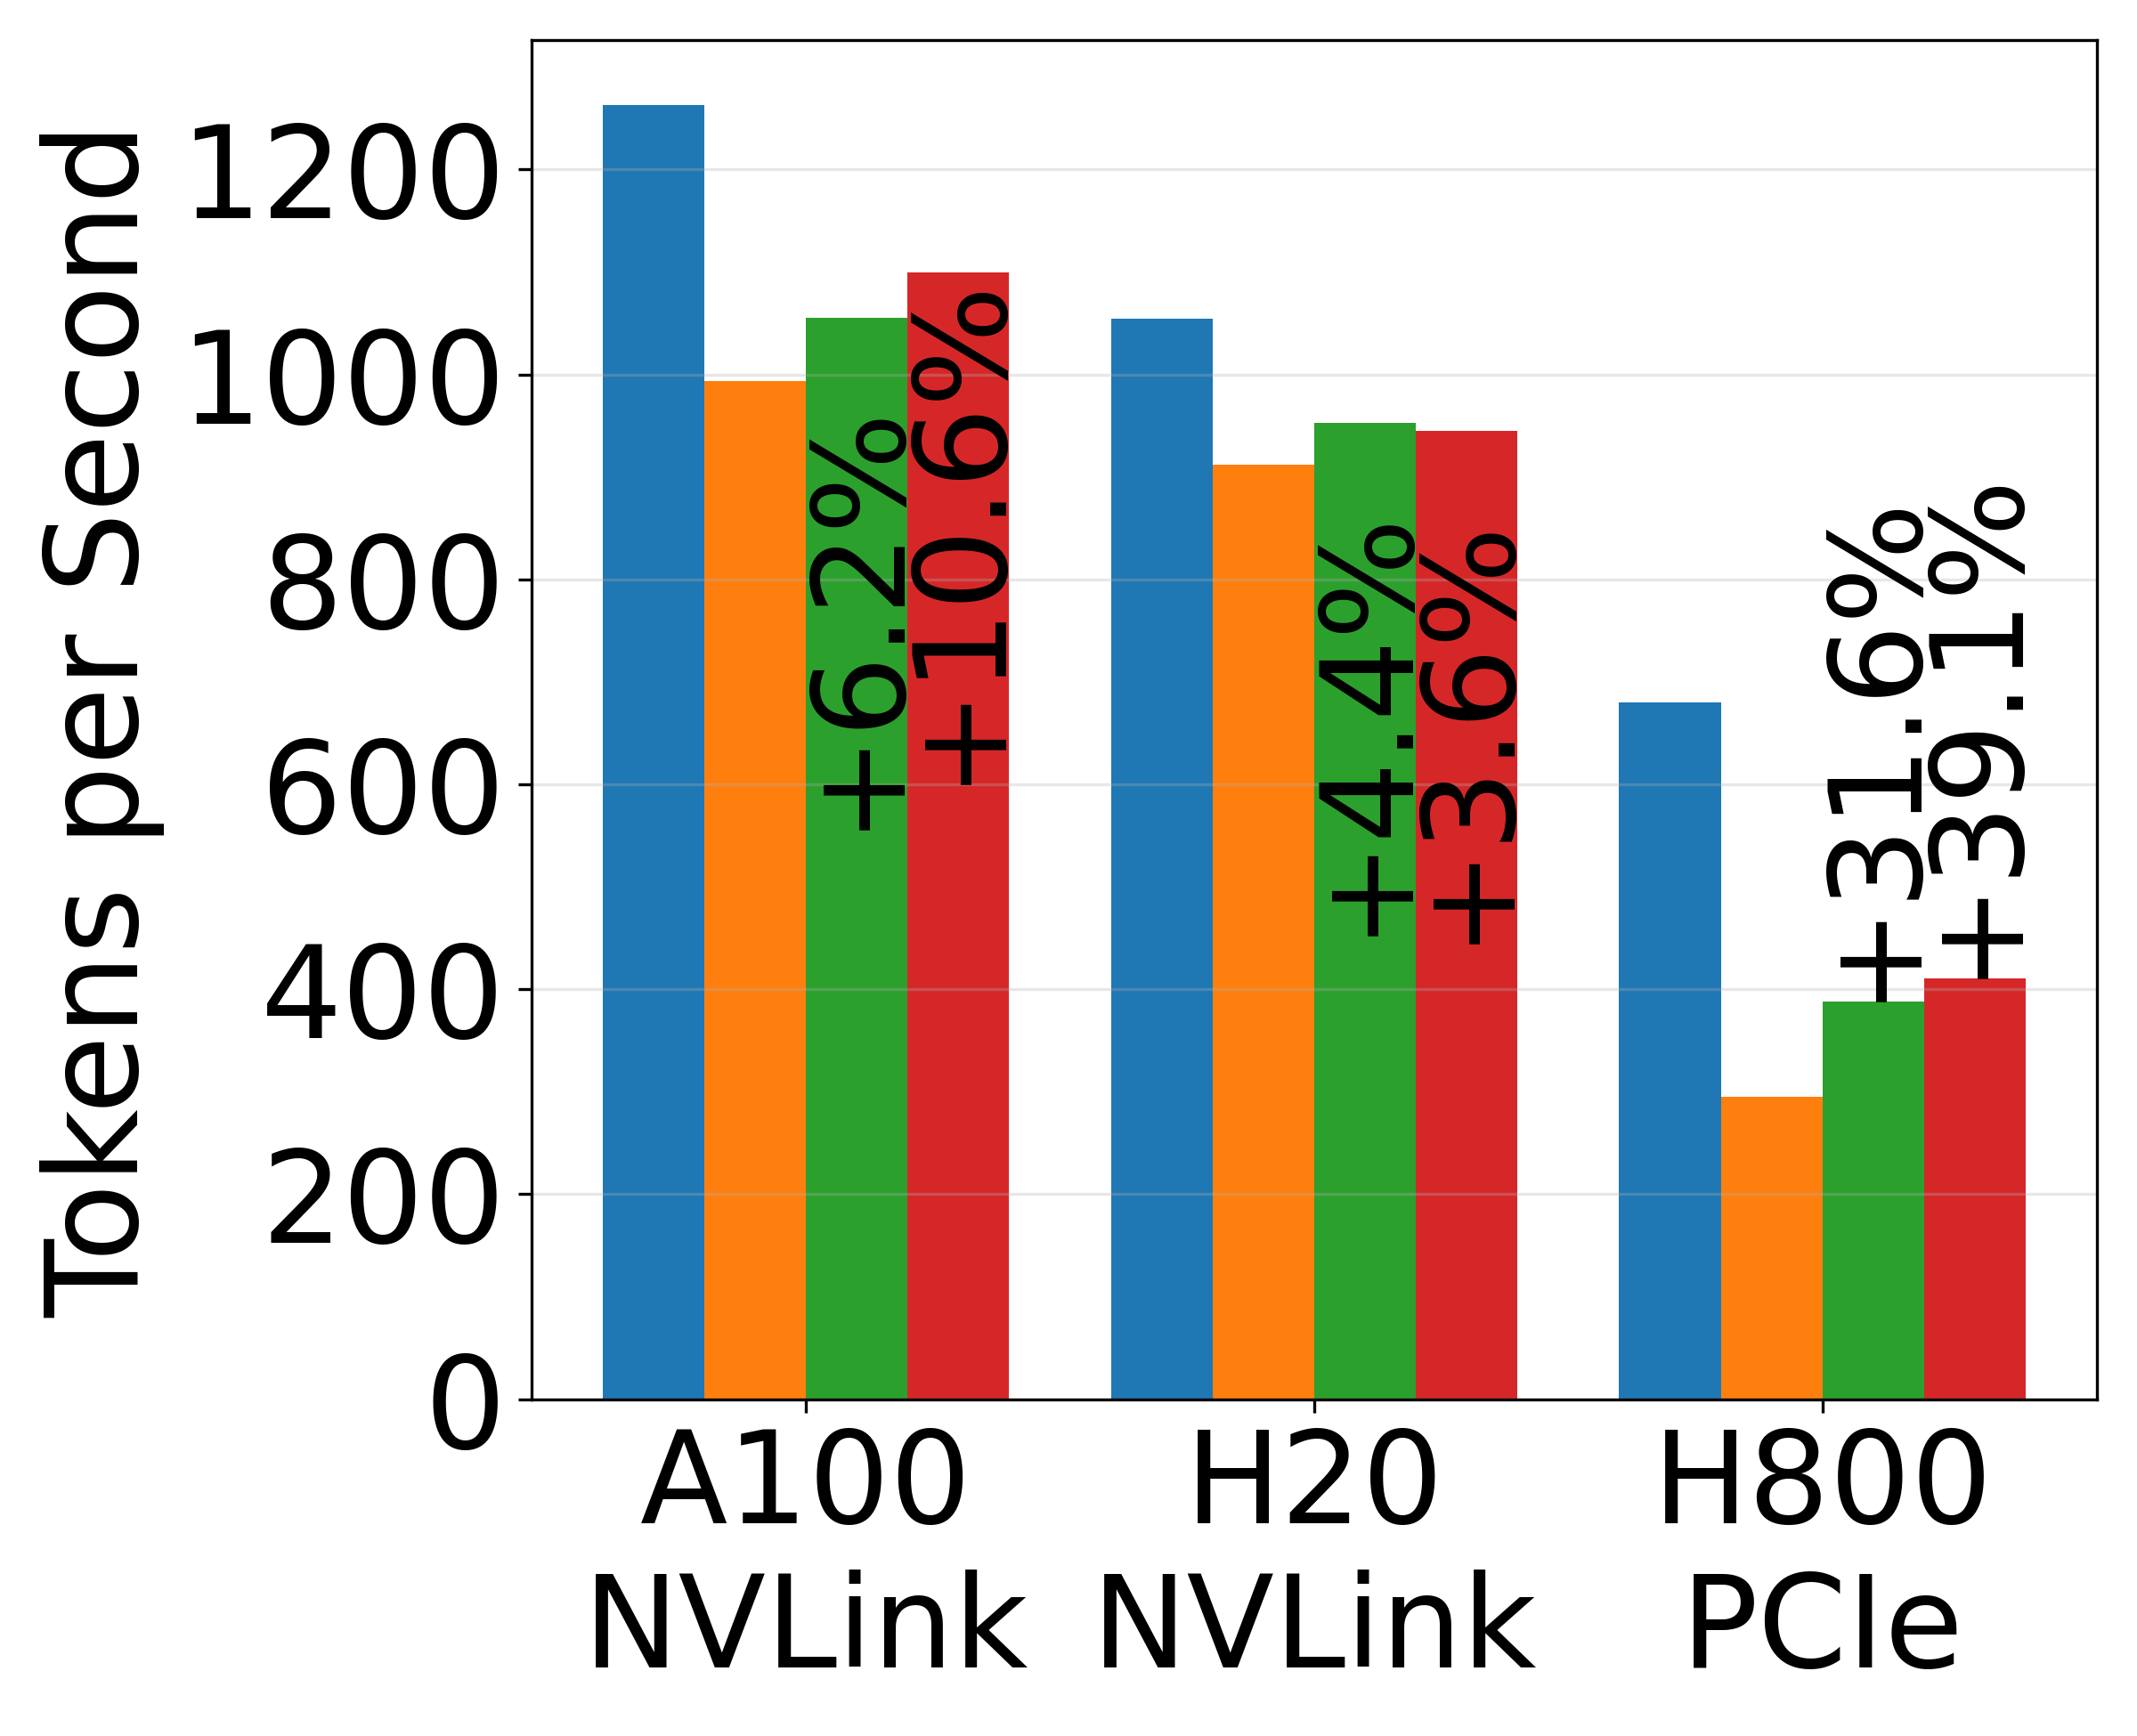
\includegraphics[width=\linewidth]{figures/hardware_comparison_b1_s1024_tokens_per_sec_qwen3-14b.png}
    \vspace{-1.5em}
    \caption{14B|B=128|S=1K}
  \end{subfigure}
  \begin{subfigure}{0.322\linewidth}
    \centering
    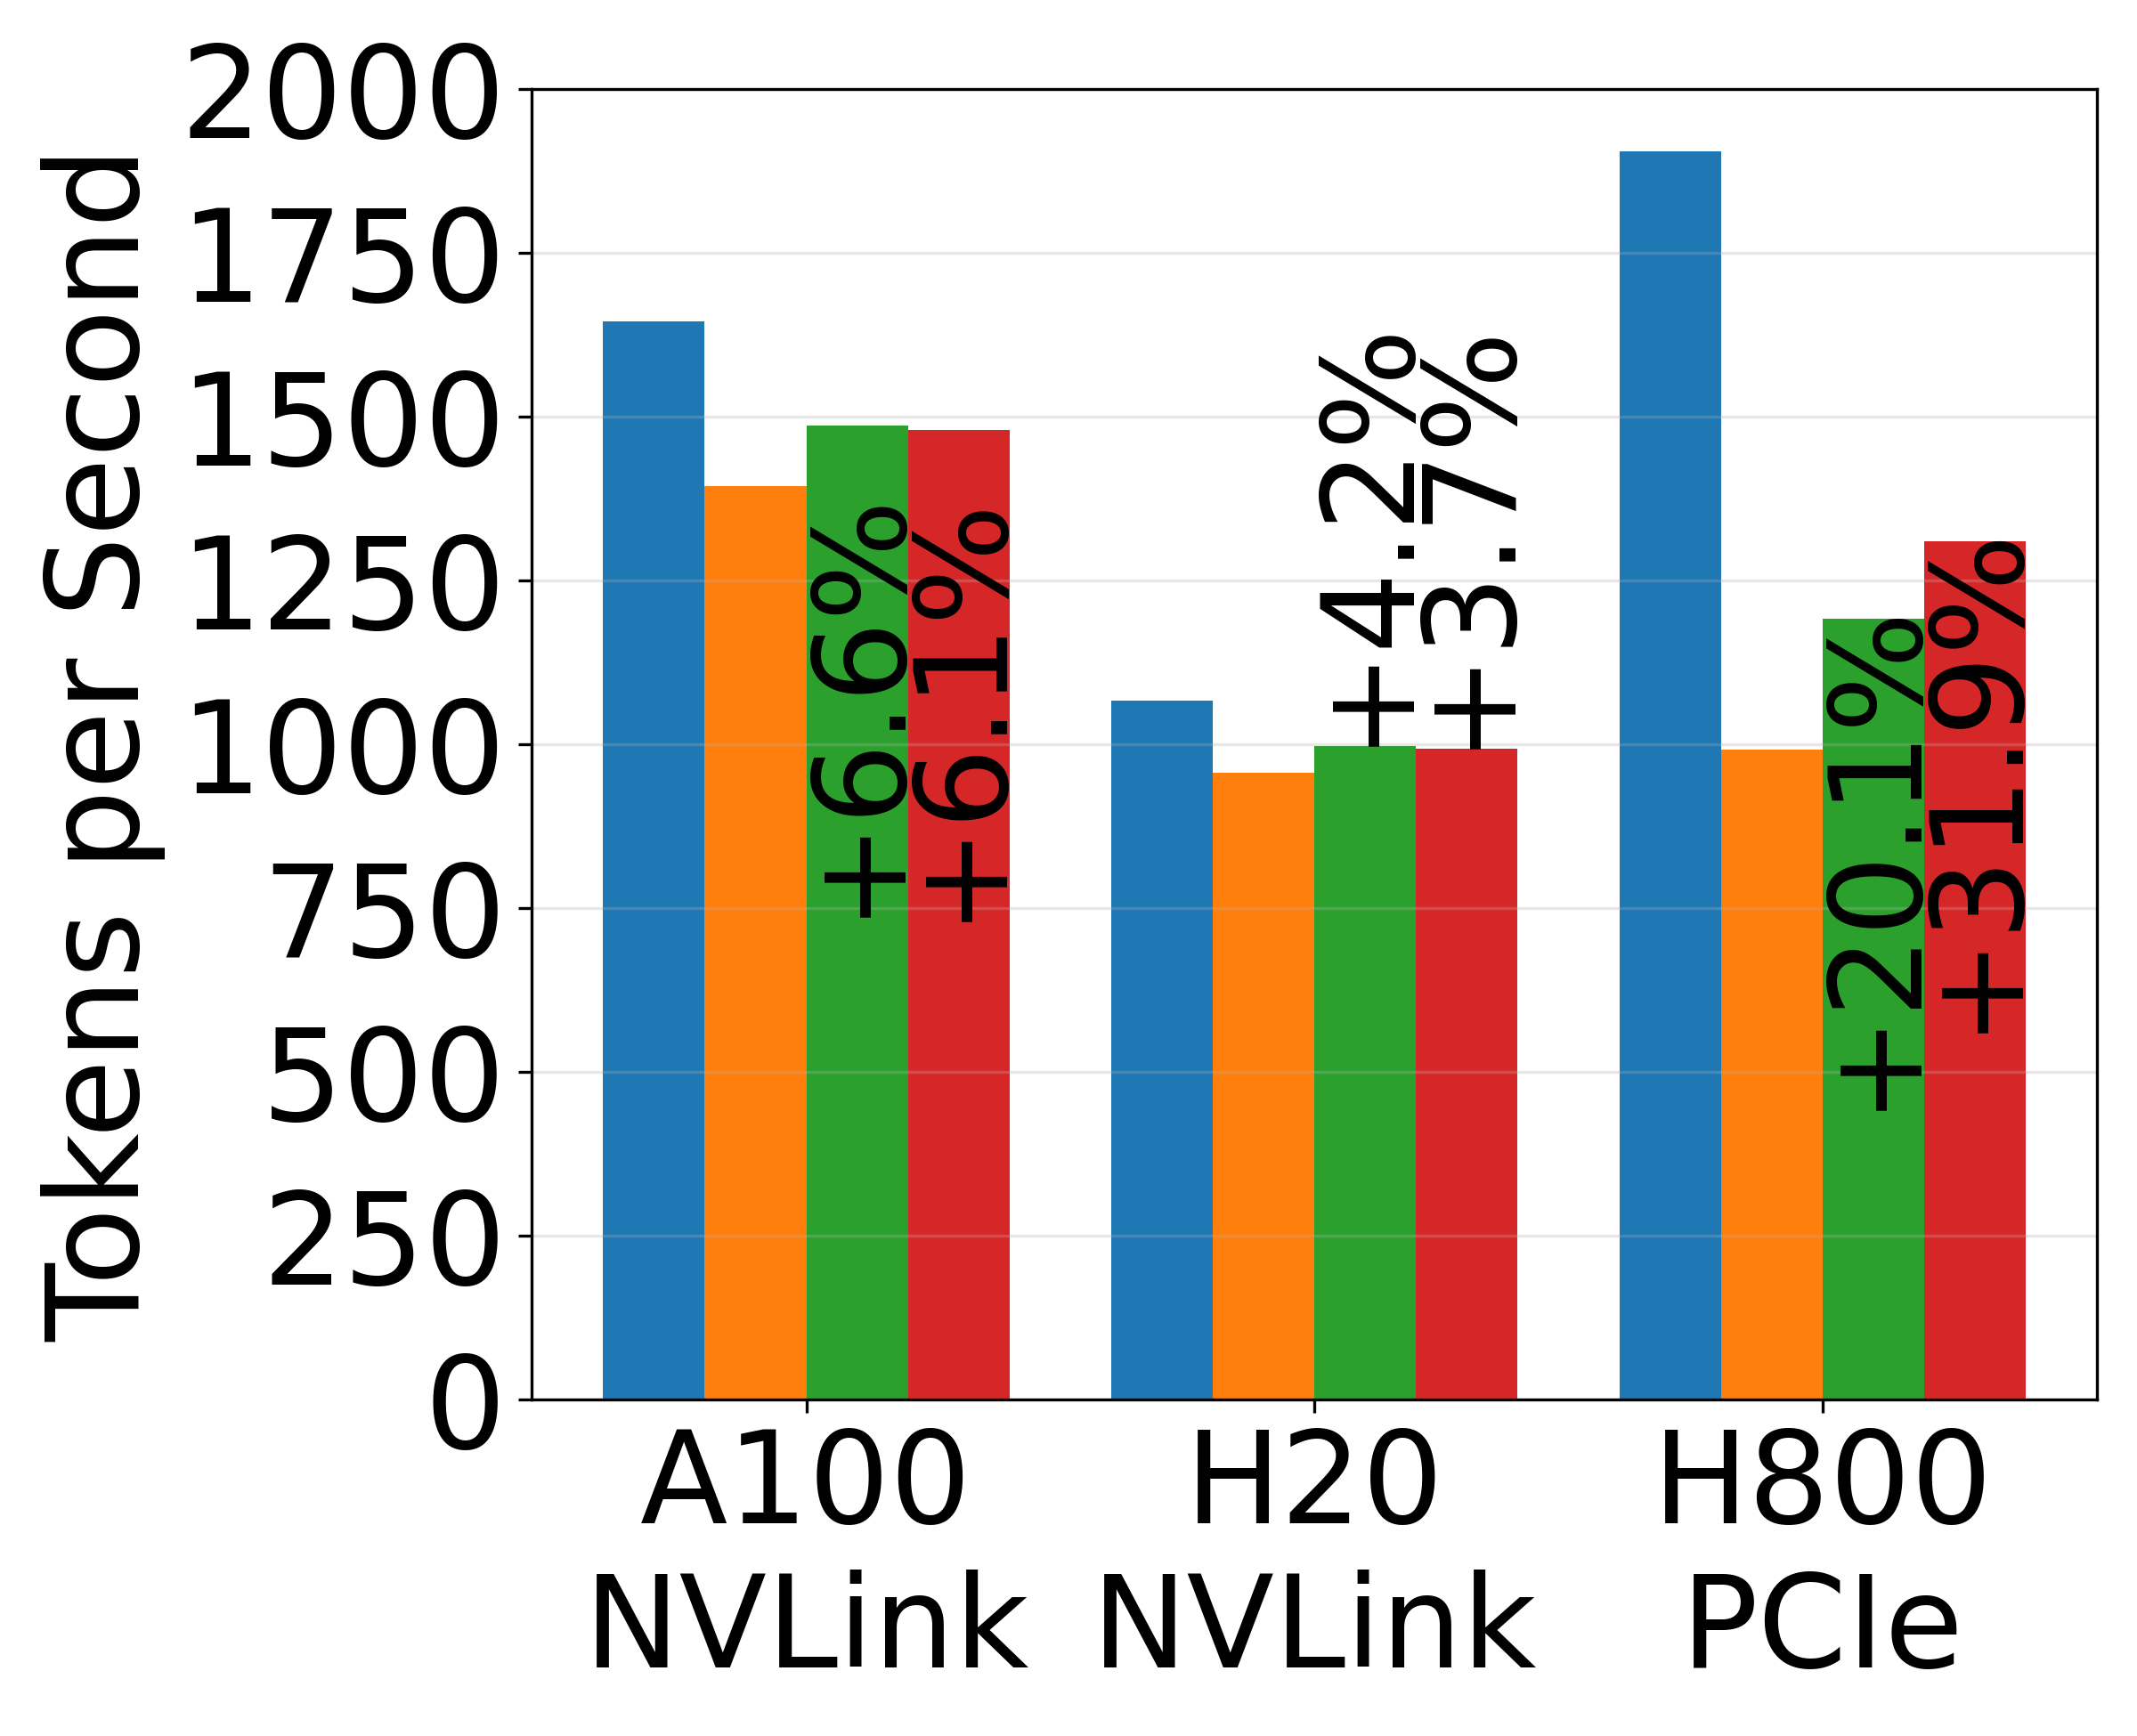
\includegraphics[width=\linewidth]{figures/hardware_comparison_b1_s2048_tokens_per_sec_qwen3-14b.png}
    \vspace{-1.5em}
    \caption{14B|B=128|S=2K}
  \end{subfigure}
  \begin{subfigure}{0.336\linewidth}
    \centering
    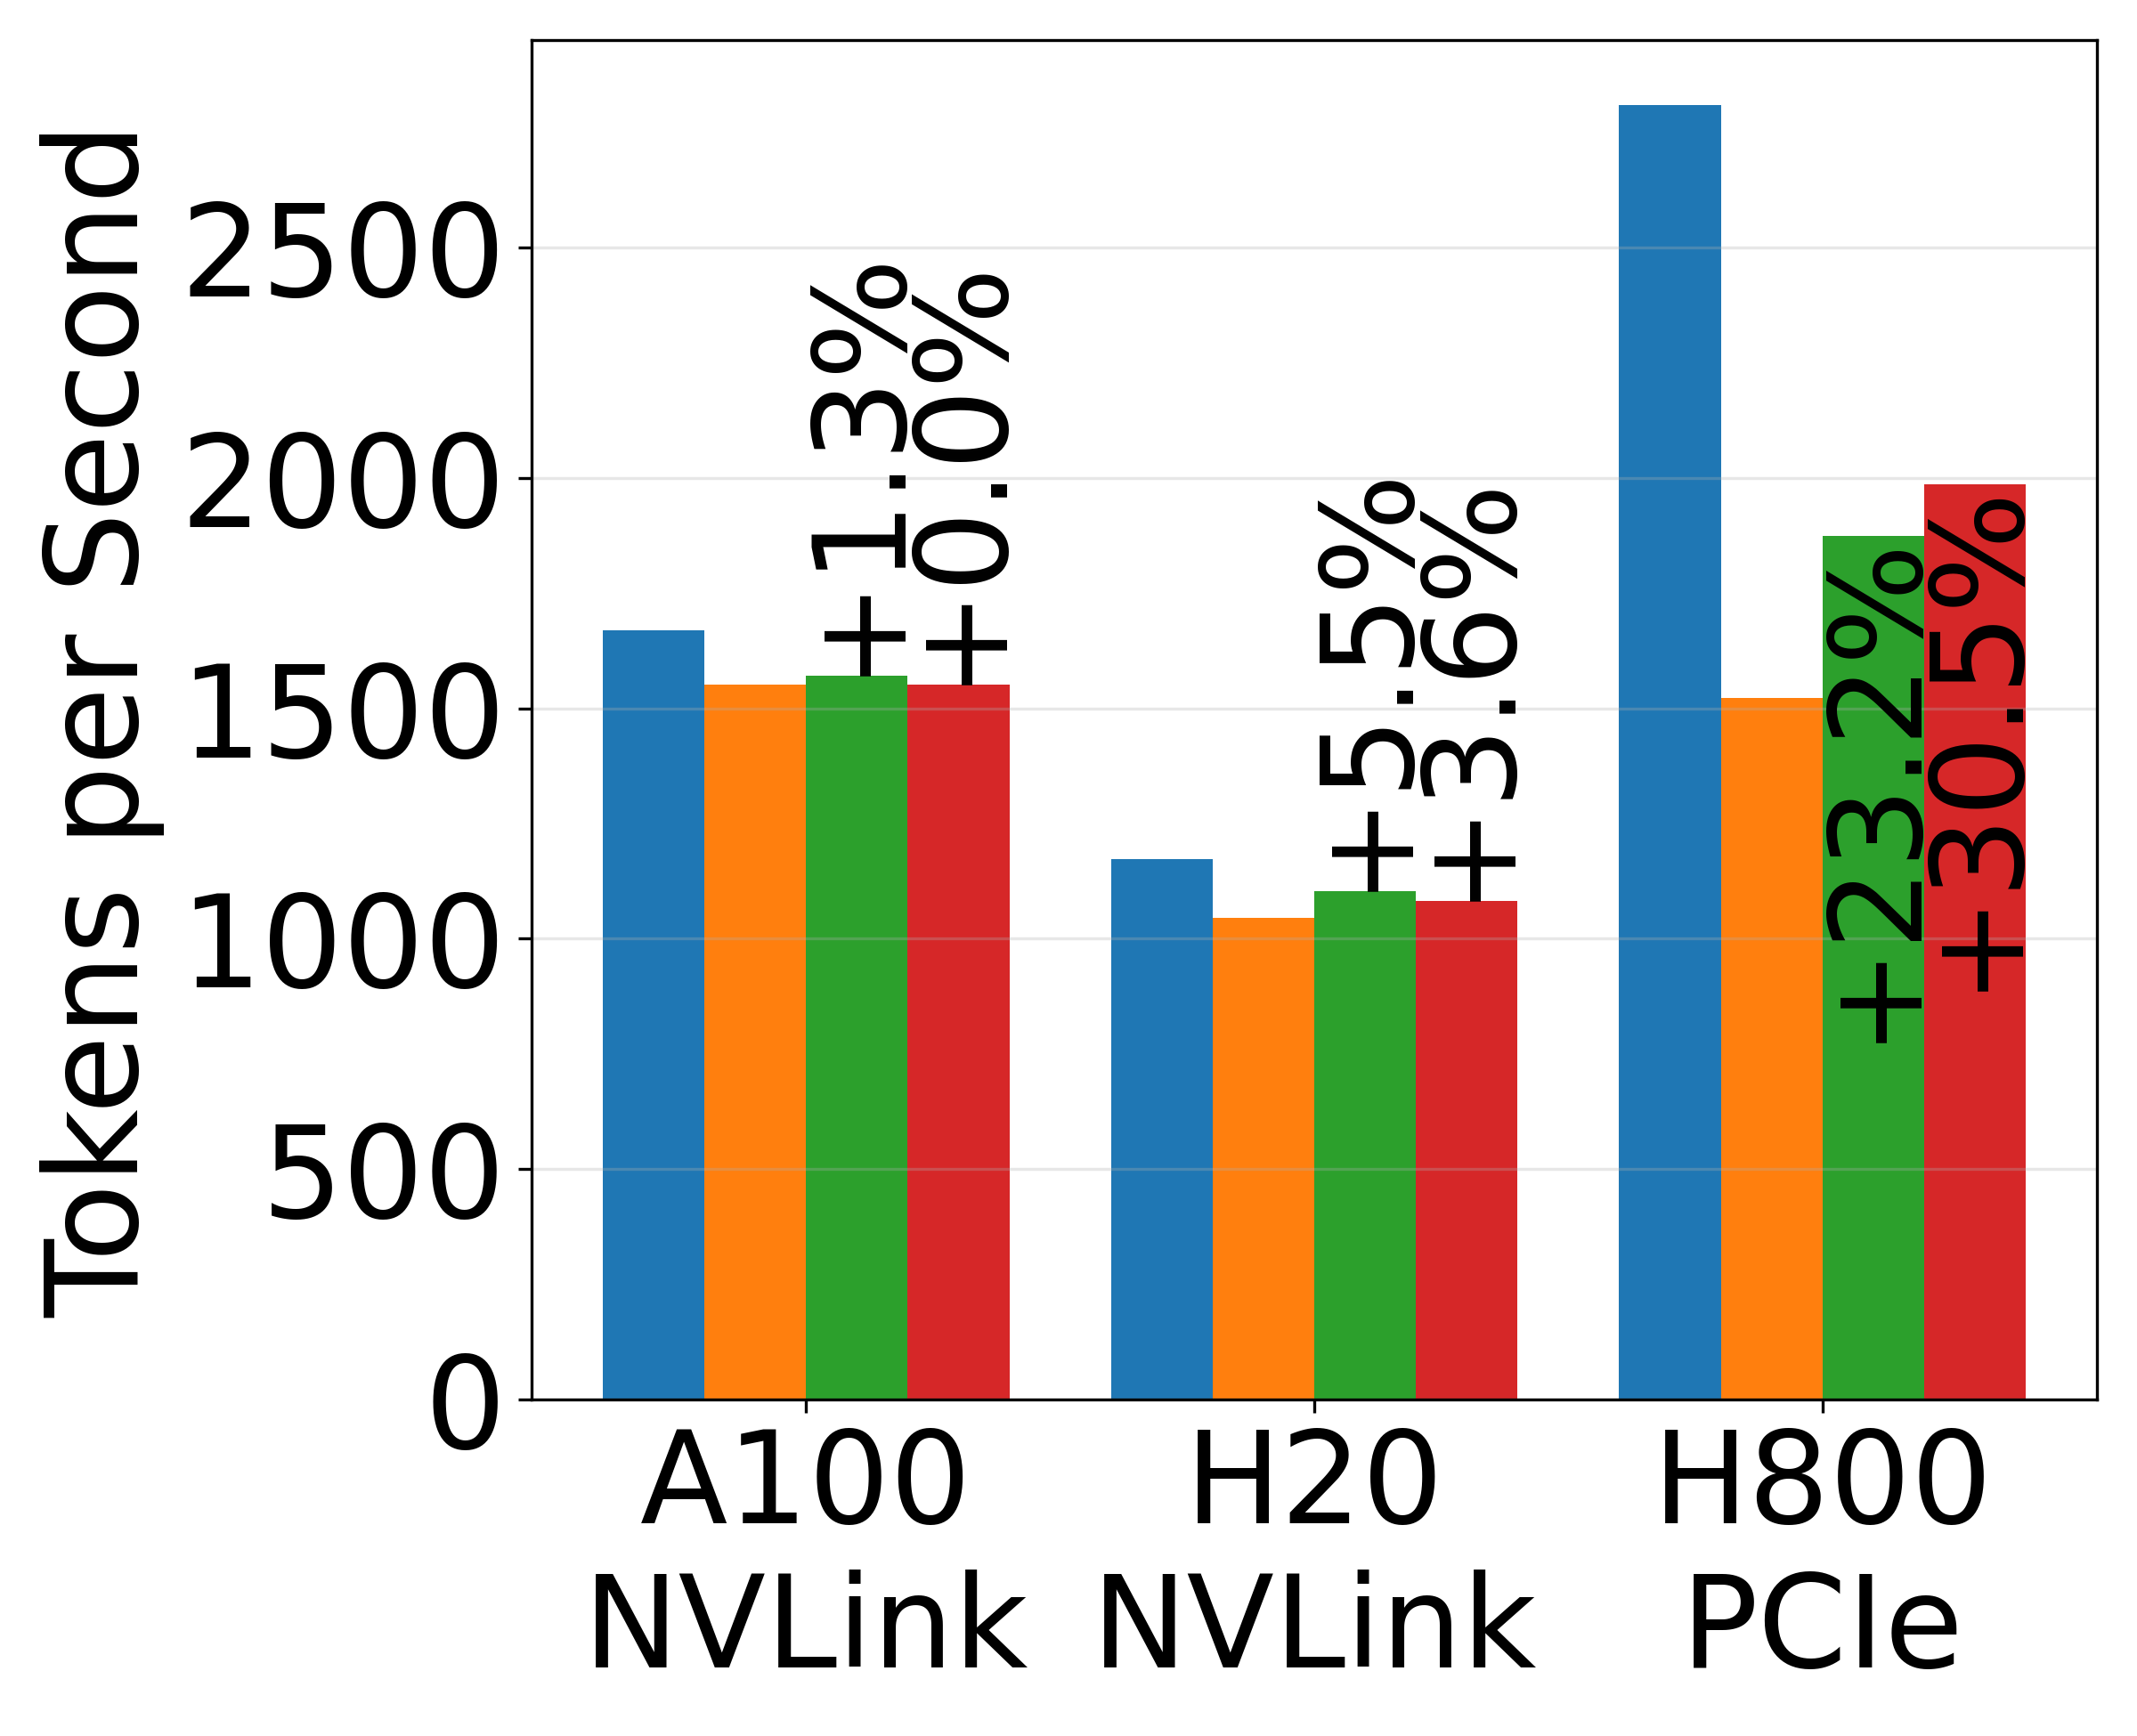
\includegraphics[width=0.972\linewidth]{figures/hardware_comparison_b2_s1536_tokens_per_sec_qwen3-14b.png}
    \vspace{-1.5em}
    \caption{14B|B=256|S=1.5K}
  \end{subfigure}
  \begin{subfigure}{0.515\linewidth}
    \centering
    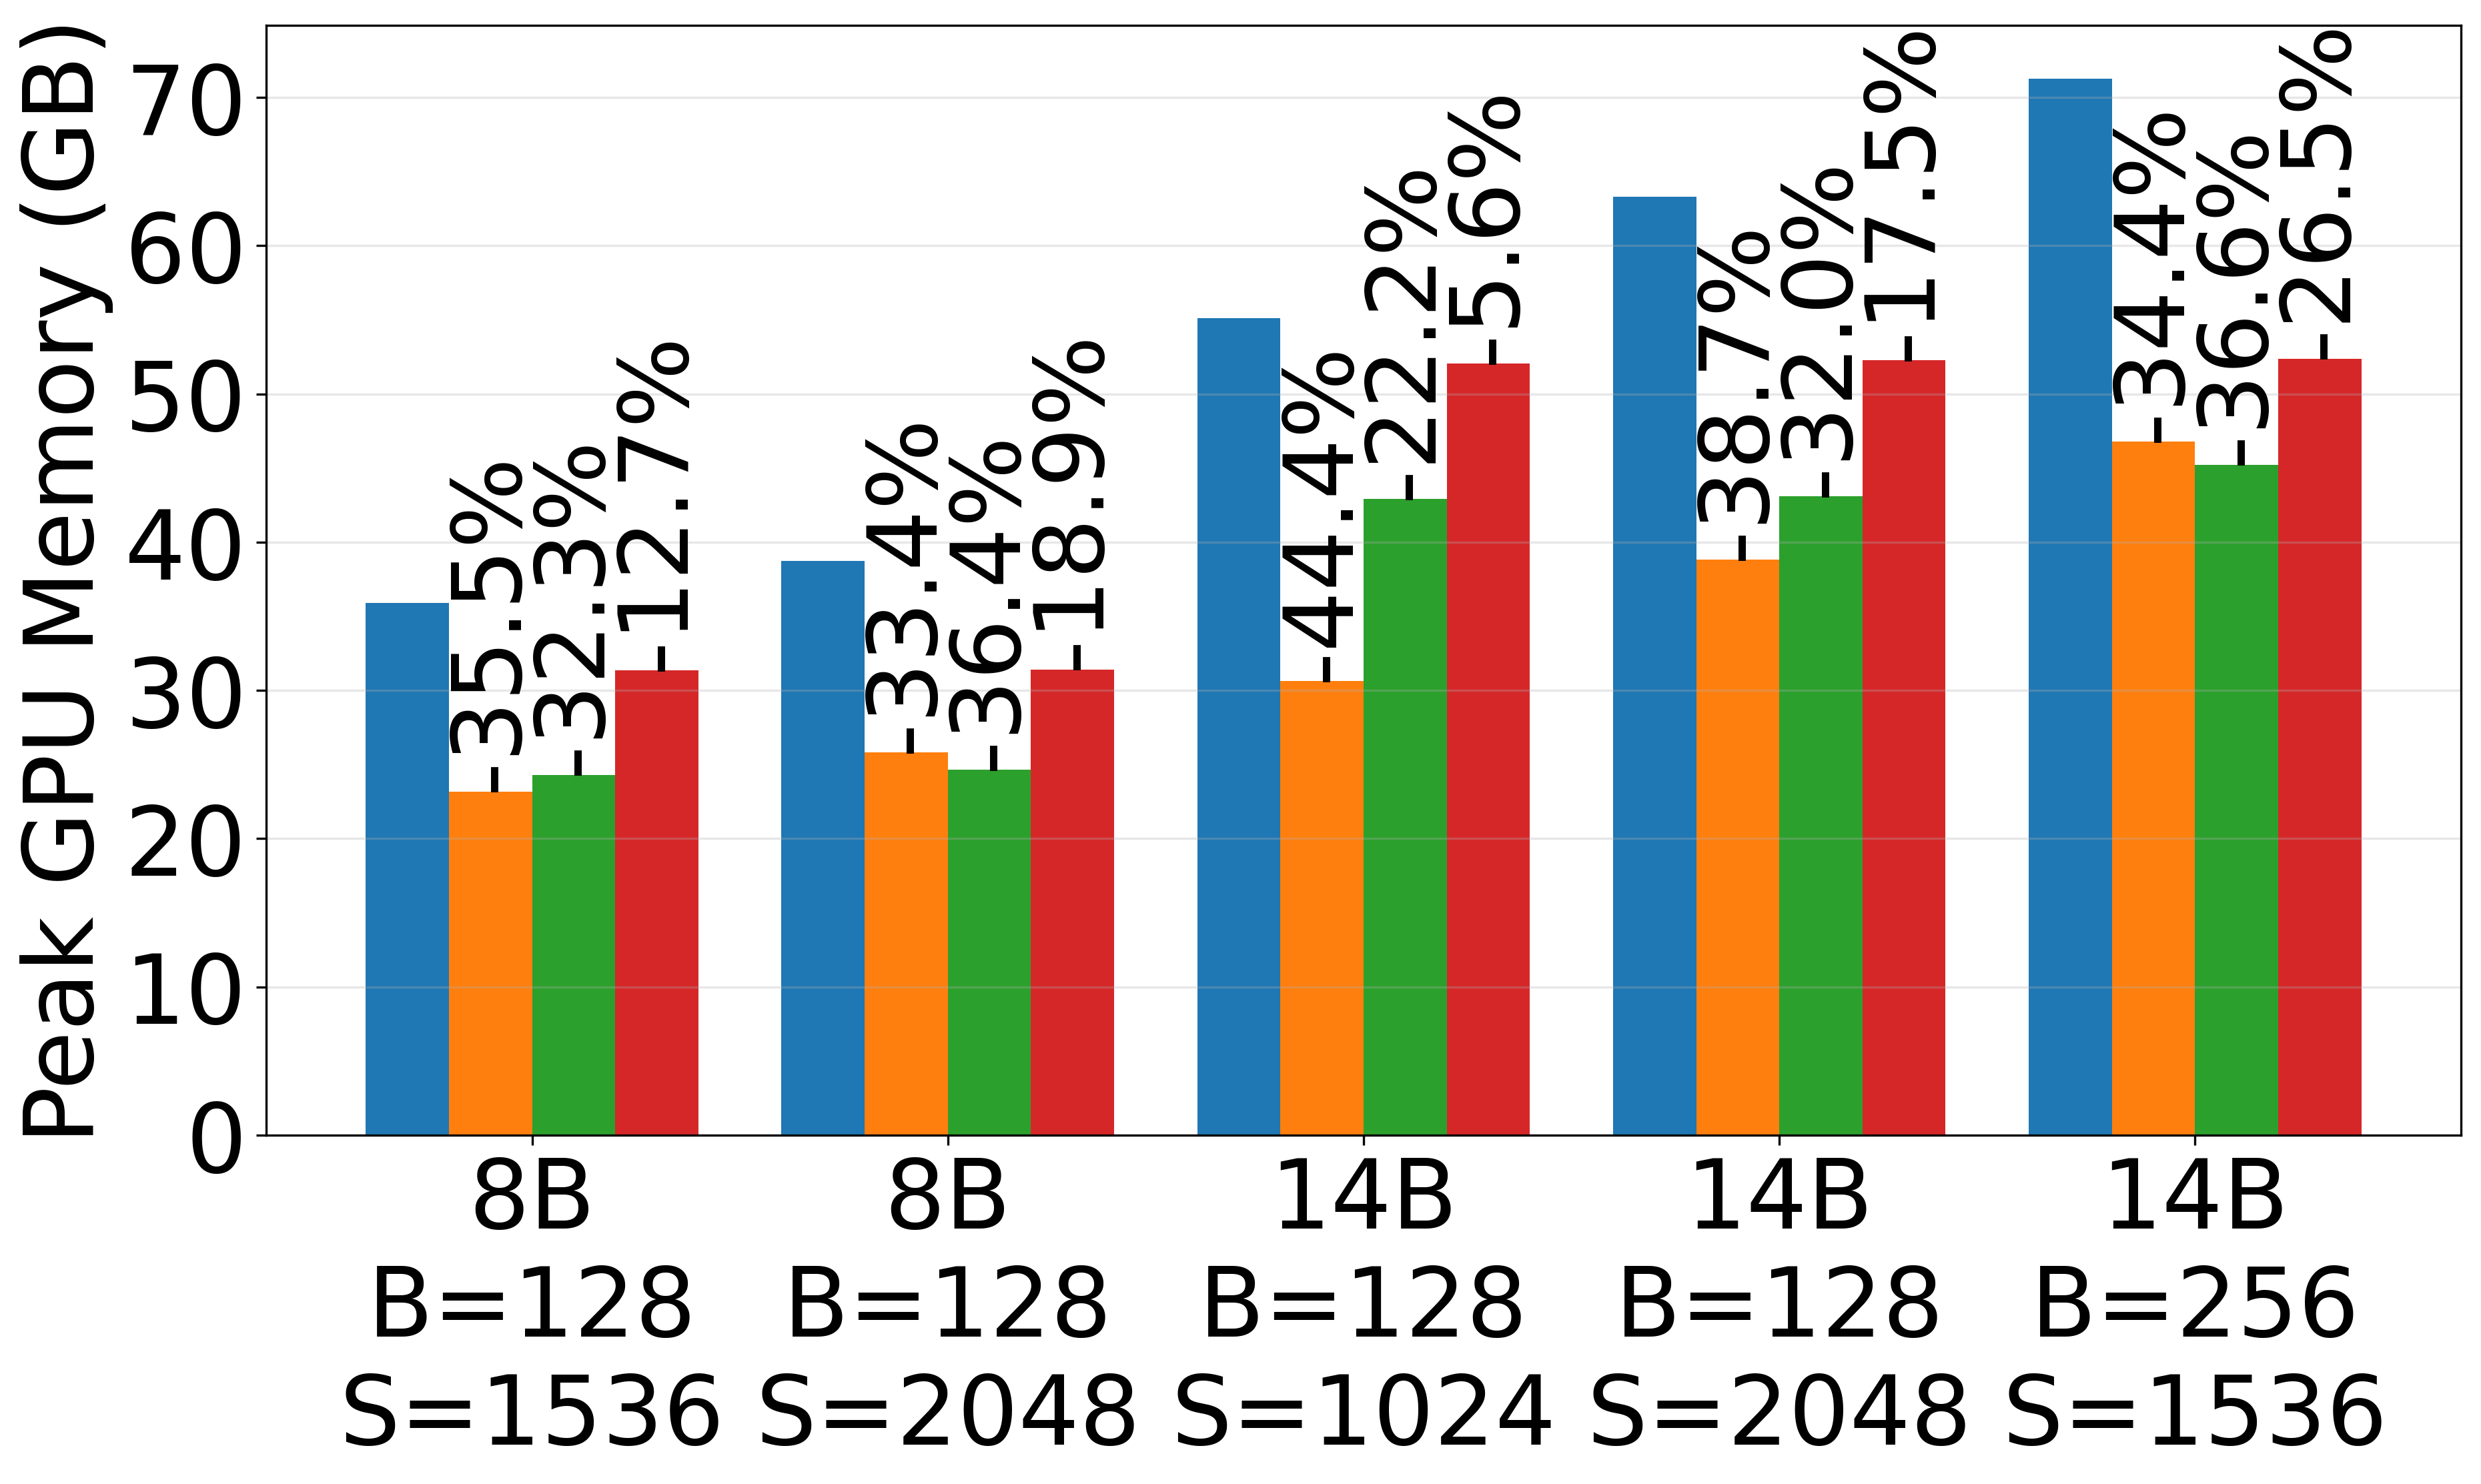
\includegraphics[width=\linewidth]{figures/memory_comparison_a100_nvlink.png}
    \vspace{-1.5em}
    \caption{Peak Memory (vs ZeRO-2)}
  \end{subfigure}
  \begin{subfigure}{0.475\linewidth}
    \centering
    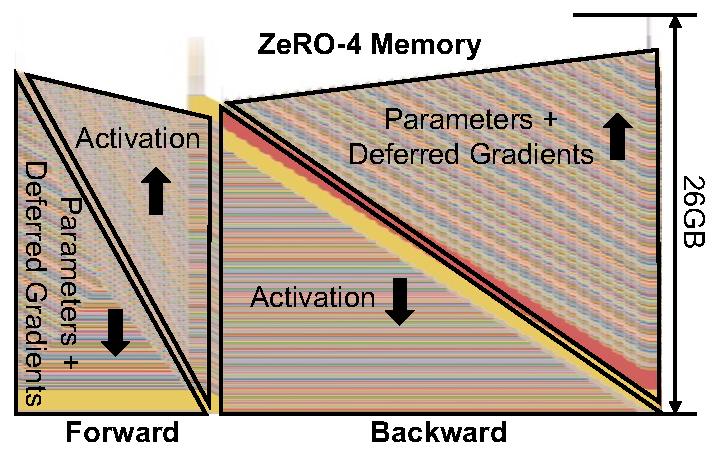
\includegraphics[width=\linewidth]{figures/zero4_memory.pdf}
    \vspace{-1.5em}
    \caption{Memory Snapshot}
  \end{subfigure}
  \vspace{-1.8em}
  \caption{Comparison of ZeRO-2, ZeRO-3, ZeRO-3.5, and ZeRO-4 in terms of performance (baseline: ZeRO-3) and memory footprint (baseline: ZeRO-2).}
  \vspace{-1.5em}
  \label{fig:zero_comparison}
\end{figure}


Fig.~\ref{fig:zero_comparison}(g) shows a memory snapshot of ZeRO-4 for Qwen3-8B (batch size = 256; seq\_len = 1.5K; memory for optimizer states, 32-bit parameters, and gradients is omitted since these are identical across strategies): peak activation memory = 26\,GB; total 16-bit parameter memory = 16\,GB; and 1/4 of gradient buckets deferred to the next forward pass, so parameters plus deferred gradients occupy 21\,GB. Let $P$ denote parameter memory, $\alpha$ the fraction of parameters retained during the backward pass, and $\beta$ the fraction of gradients deferred to the next forward pass. If the activation peak $A$ satisfies $A \ge (\alpha+\beta)\cdot P$, then the peak memory usage of ZeRO-3, ZeRO-3.5, and ZeRO-4 is comparable (Fig.~\ref{fig:zero_comparison}(f)). 

% Hence, without increasing peak GPU memory (up to 36.5\% savings compared to ZeRO-2), these strategies can improve memory utilization and trade memory for up to a 40\% increase in throughput.

From a hardware perspective (Fig.~\ref{fig:zero_comparison}(a-d)), the performance gains of ZeRO-3.5/4 over ZeRO-3 are more pronounced on systems with lower communication bandwidth (e.g., PCIe vs. NVLink) and under lighter compute loads (since communication overhead is harder to overlap). ZeRO-3.5 eliminates the forward all-gather, and ZeRO-4 further shifts part of backward communication into the forward pass to improve communication-computation overlap, thereby yielding larger performance gains on communication-constrained systems.

\subsubsection{Configuration Exploration}

We further analyze how hyperparameters affect the performance and memory usage of ZeRO-3.5 and ZeRO-4. We vary batch size/sequence length (to vary activation memory and computation loads) and strategy-specific hyperparameters: the ratio between retained gathered parameters and released parameters during backward (ZeRO-3.5), and the ratio between reduced gradient buckets and buckets whose gradient reduce-scatter is deferred to the subsequent forward pass (ZeRO-4). For ZeRO-4 exploration, we fix the retained-parameter ratio to \texttt{ALL:0} (all gathered parameters are kept during backward).

\begin{figure}[t]
  \centering
  \begin{subfigure}{0.48\linewidth}
    \centering
    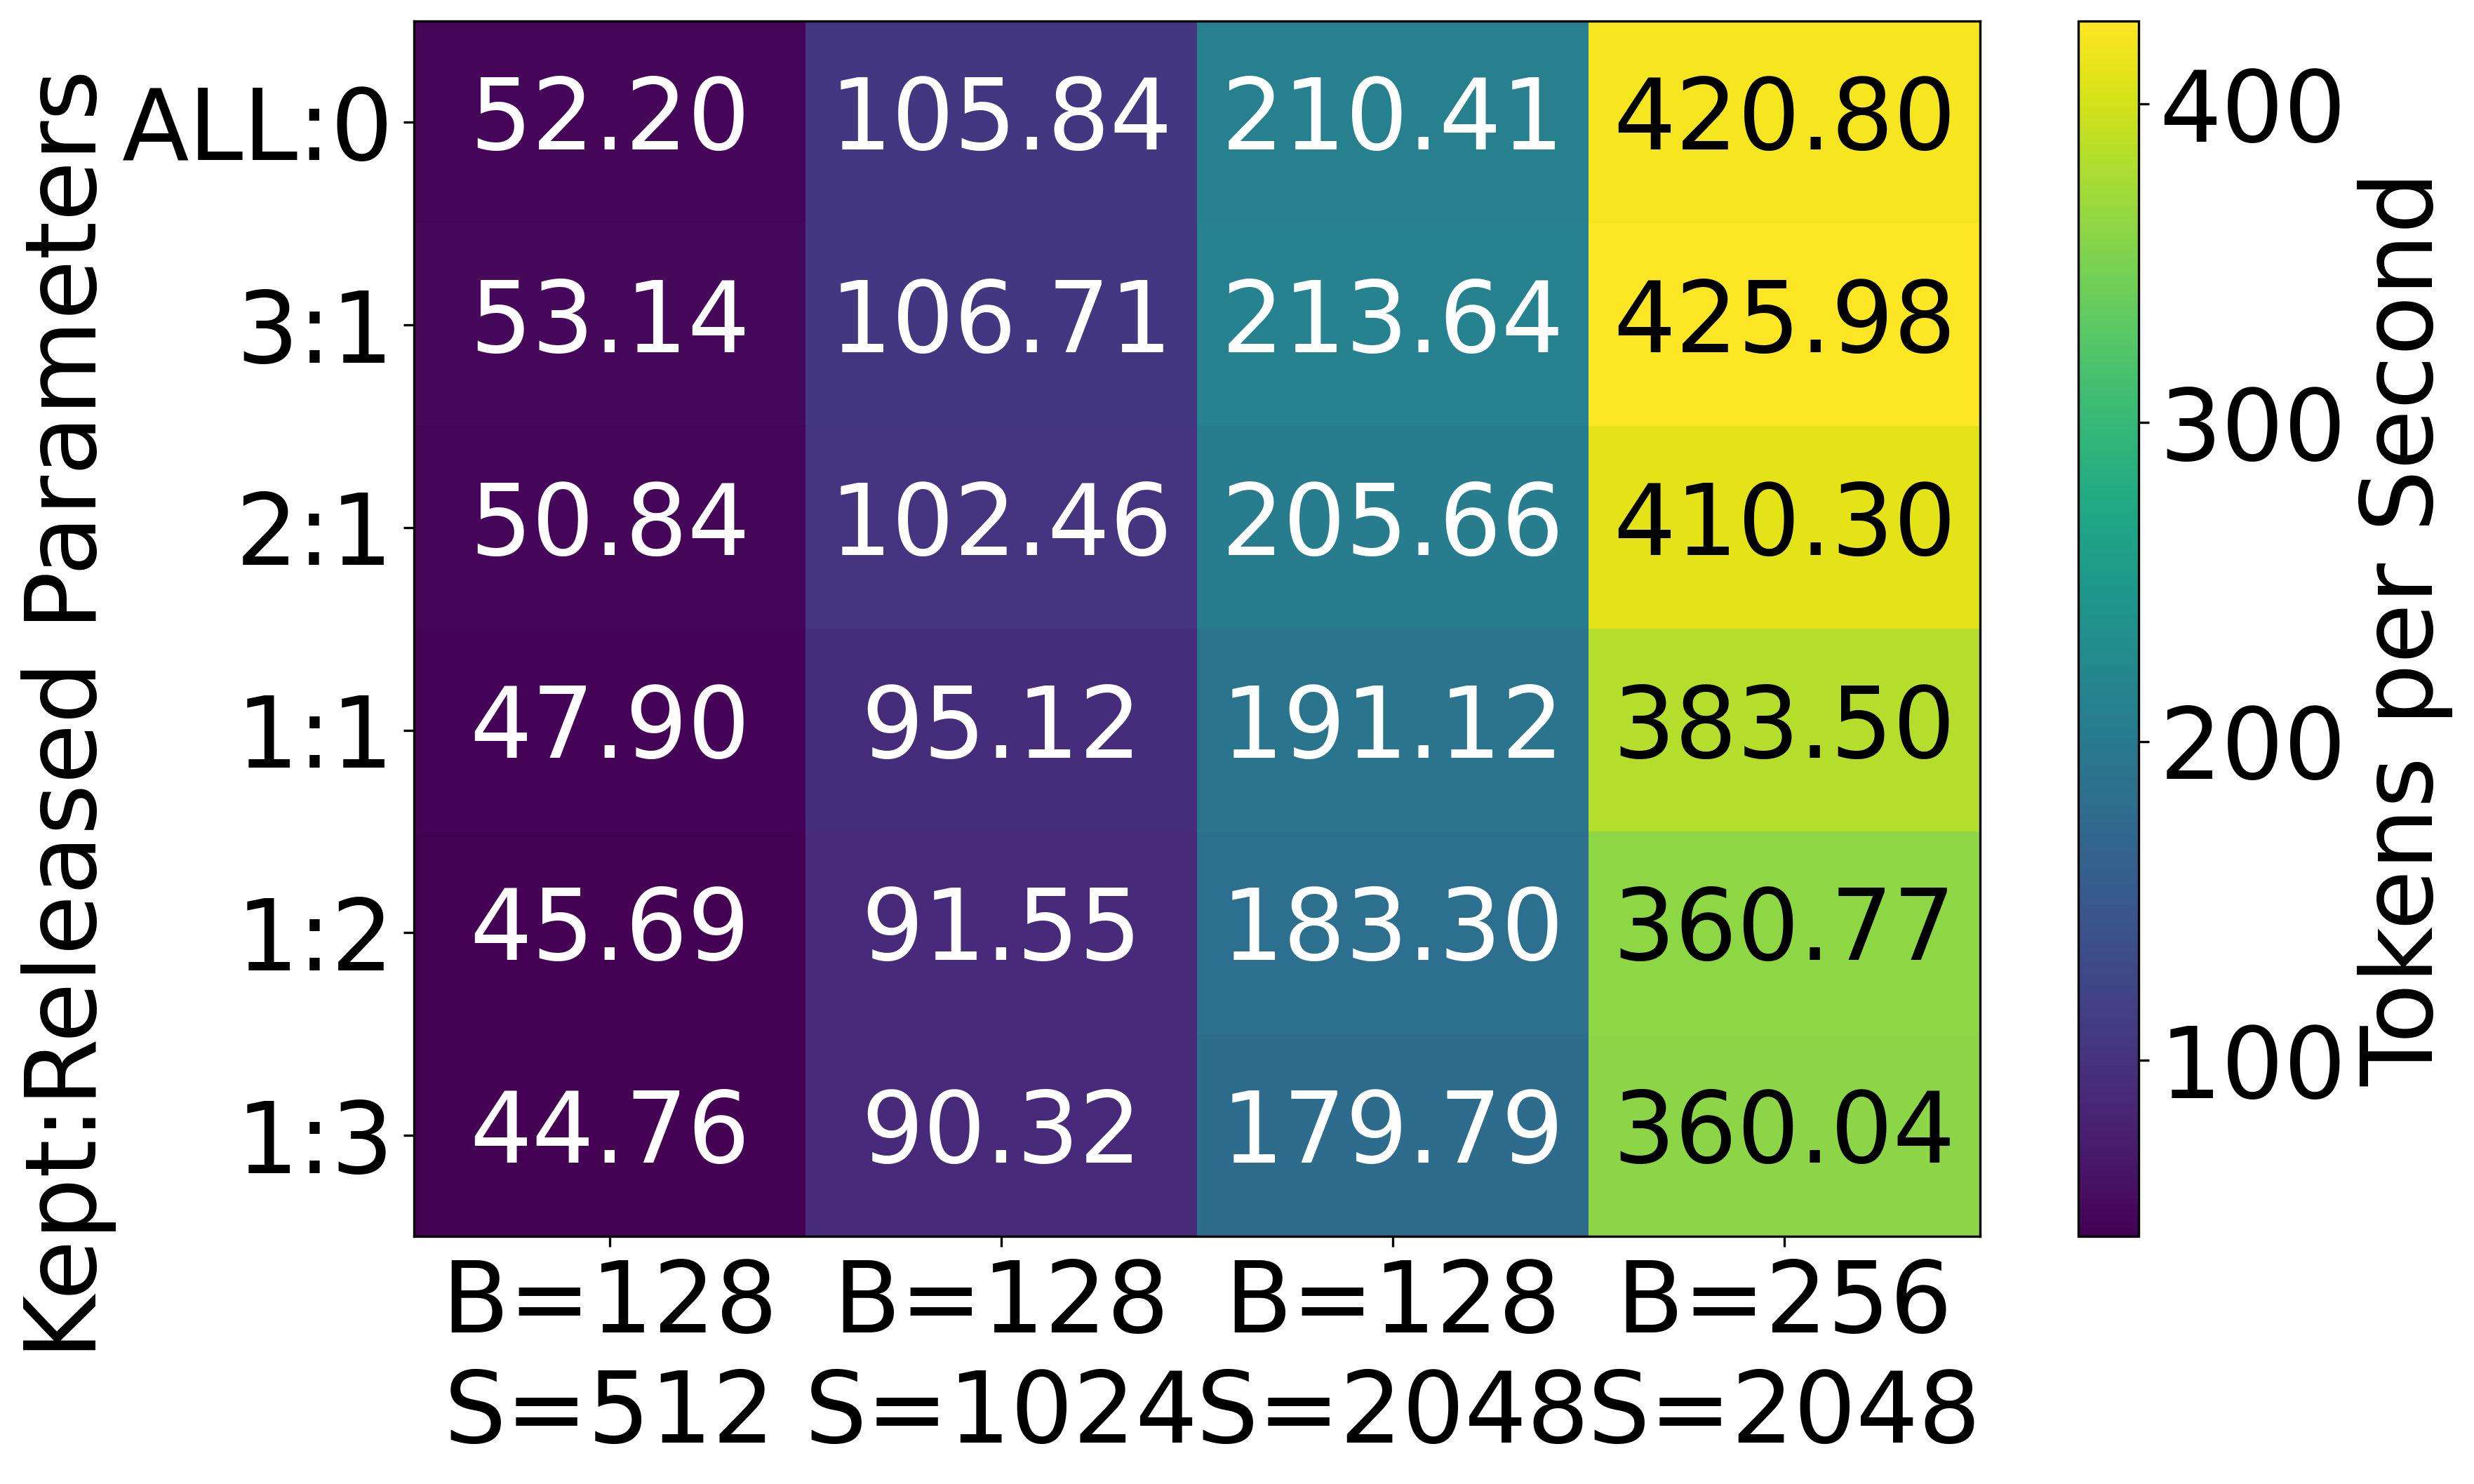
\includegraphics[width=\linewidth]{figures/strategy_3.5_ckpt_False_tokens_per_sec_heatmap.png}
    \vspace{-1.5em}
    \caption{Throughput (ZeRO-3.5)}
  \end{subfigure}
  \begin{subfigure}{0.48\linewidth}
    \centering
    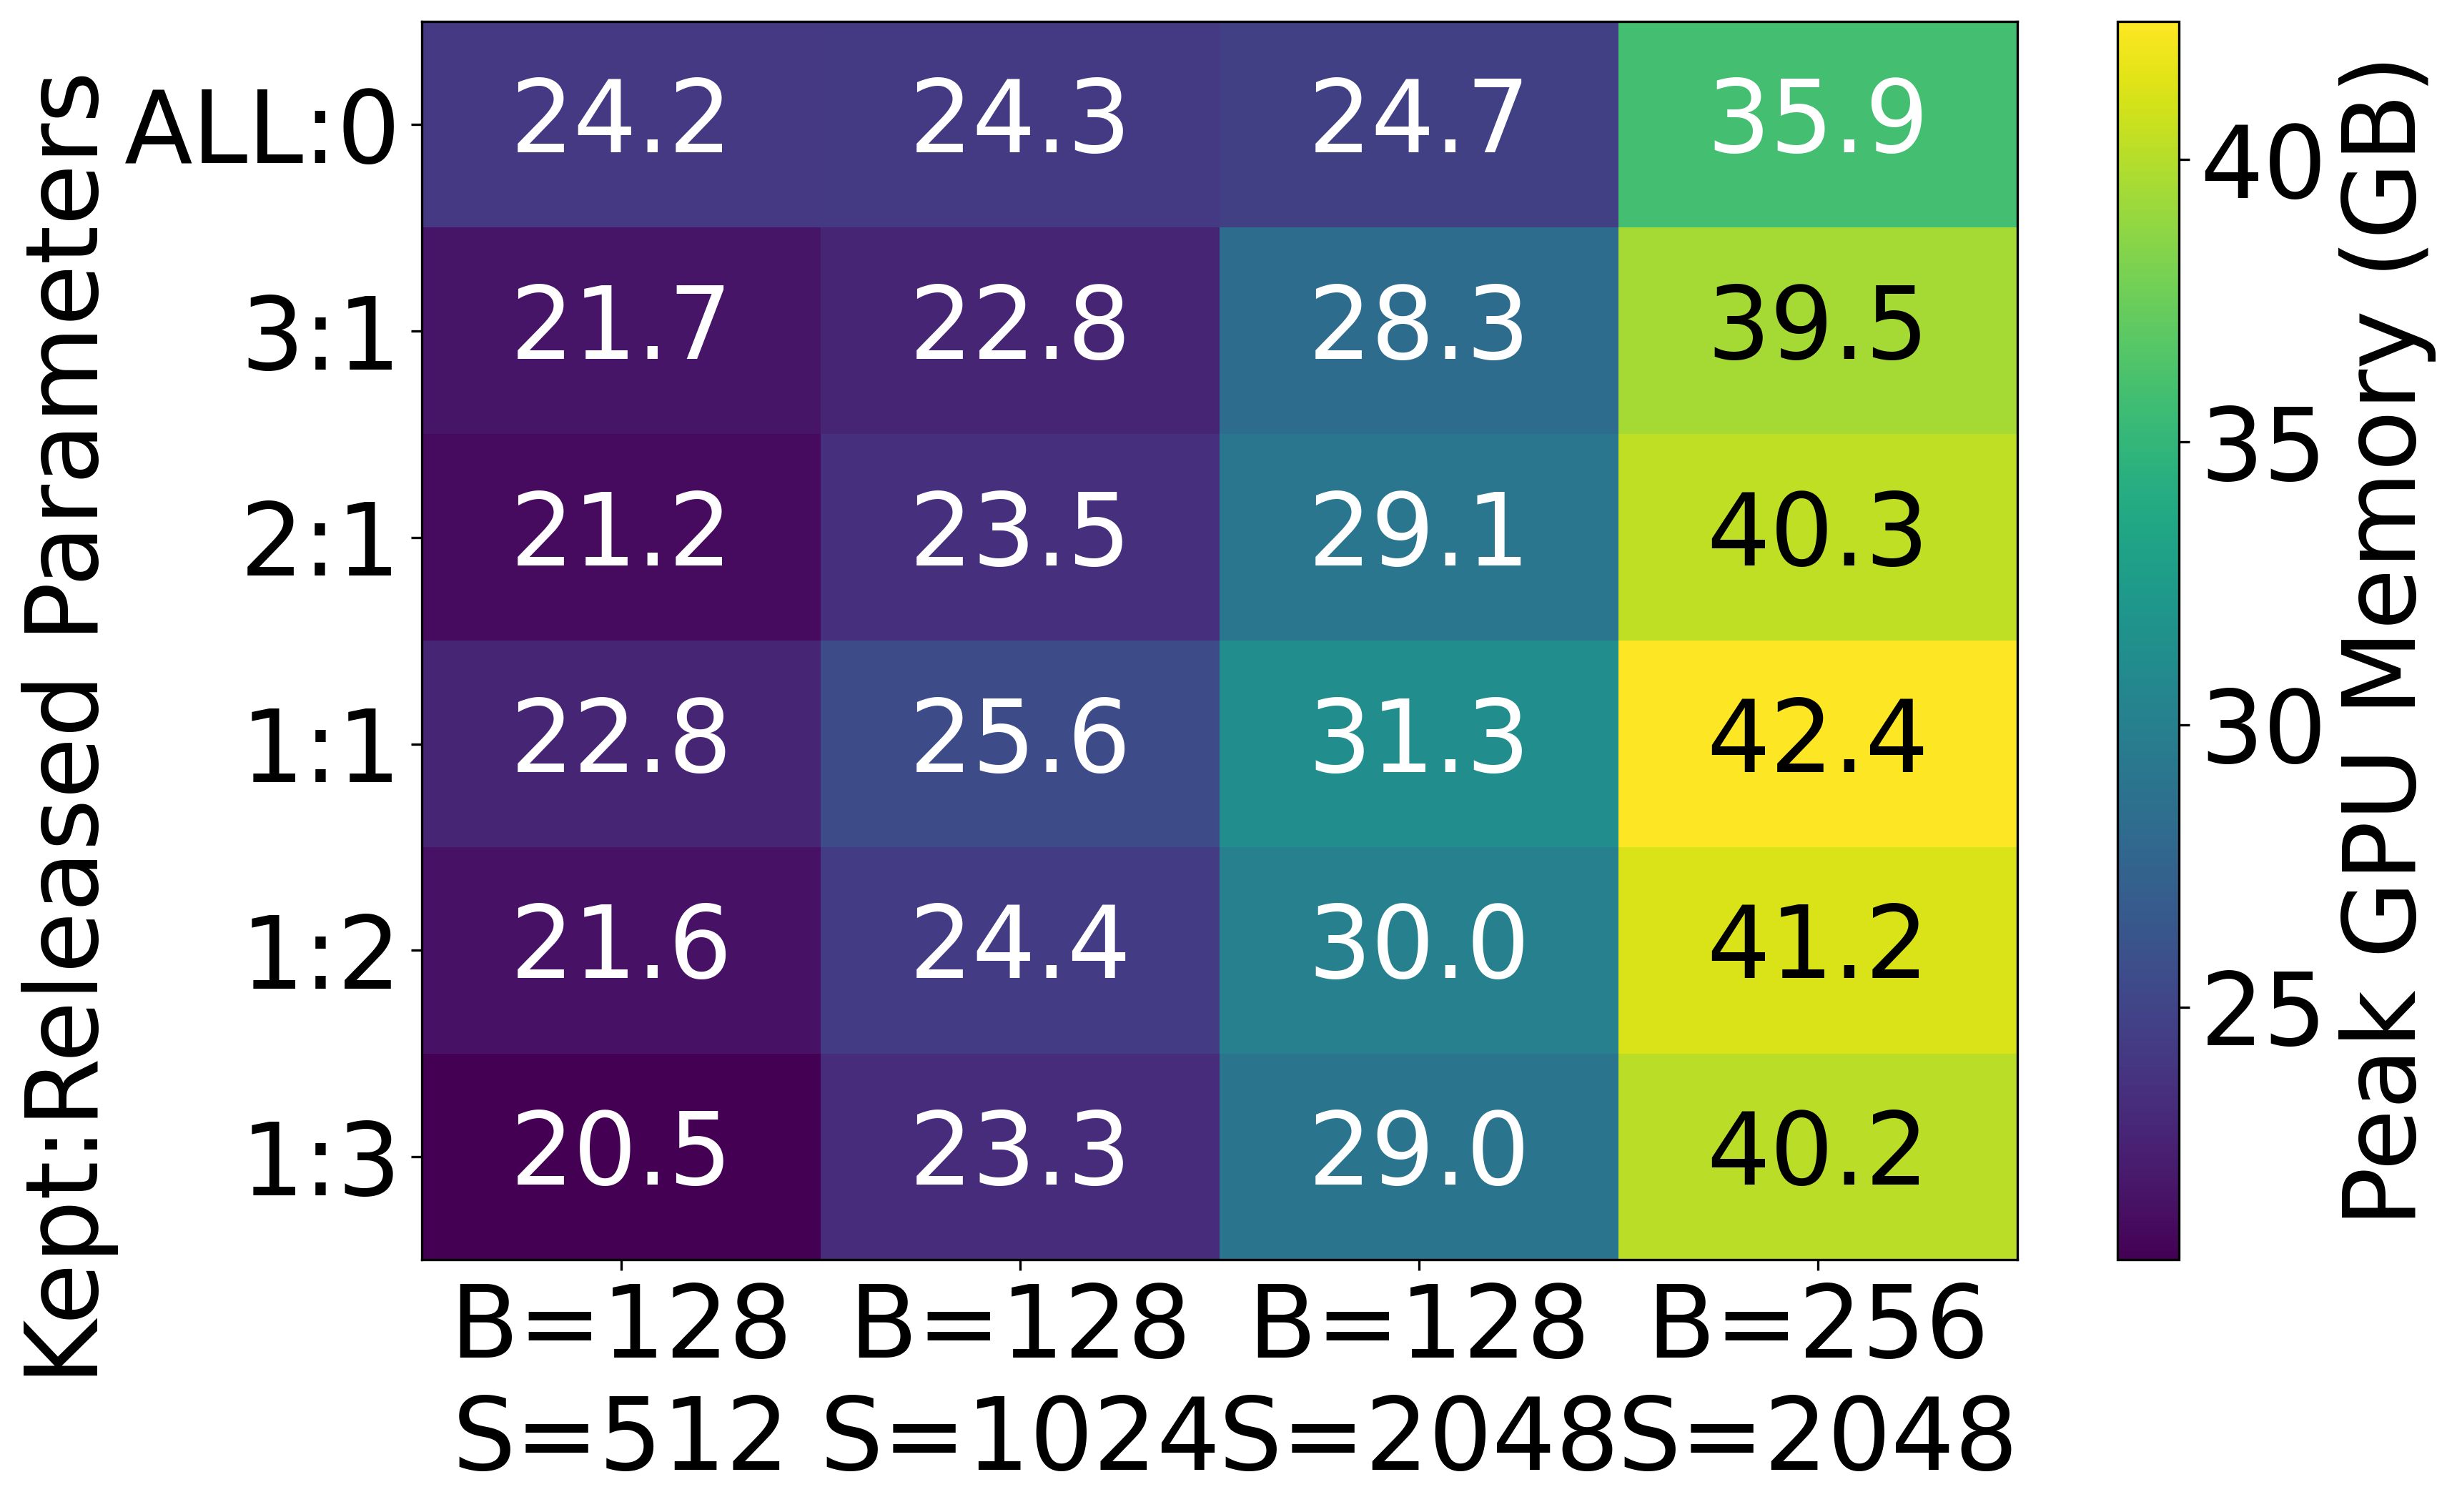
\includegraphics[width=\linewidth]{figures/strategy_3.5_ckpt_False_peak_gpu_mem_mb_heatmap.png}
    \vspace{-1.5em}
    \caption{Peak Memory (ZeRO-3.5)}
  \end{subfigure}
  \begin{subfigure}{0.48\linewidth}
    \centering
    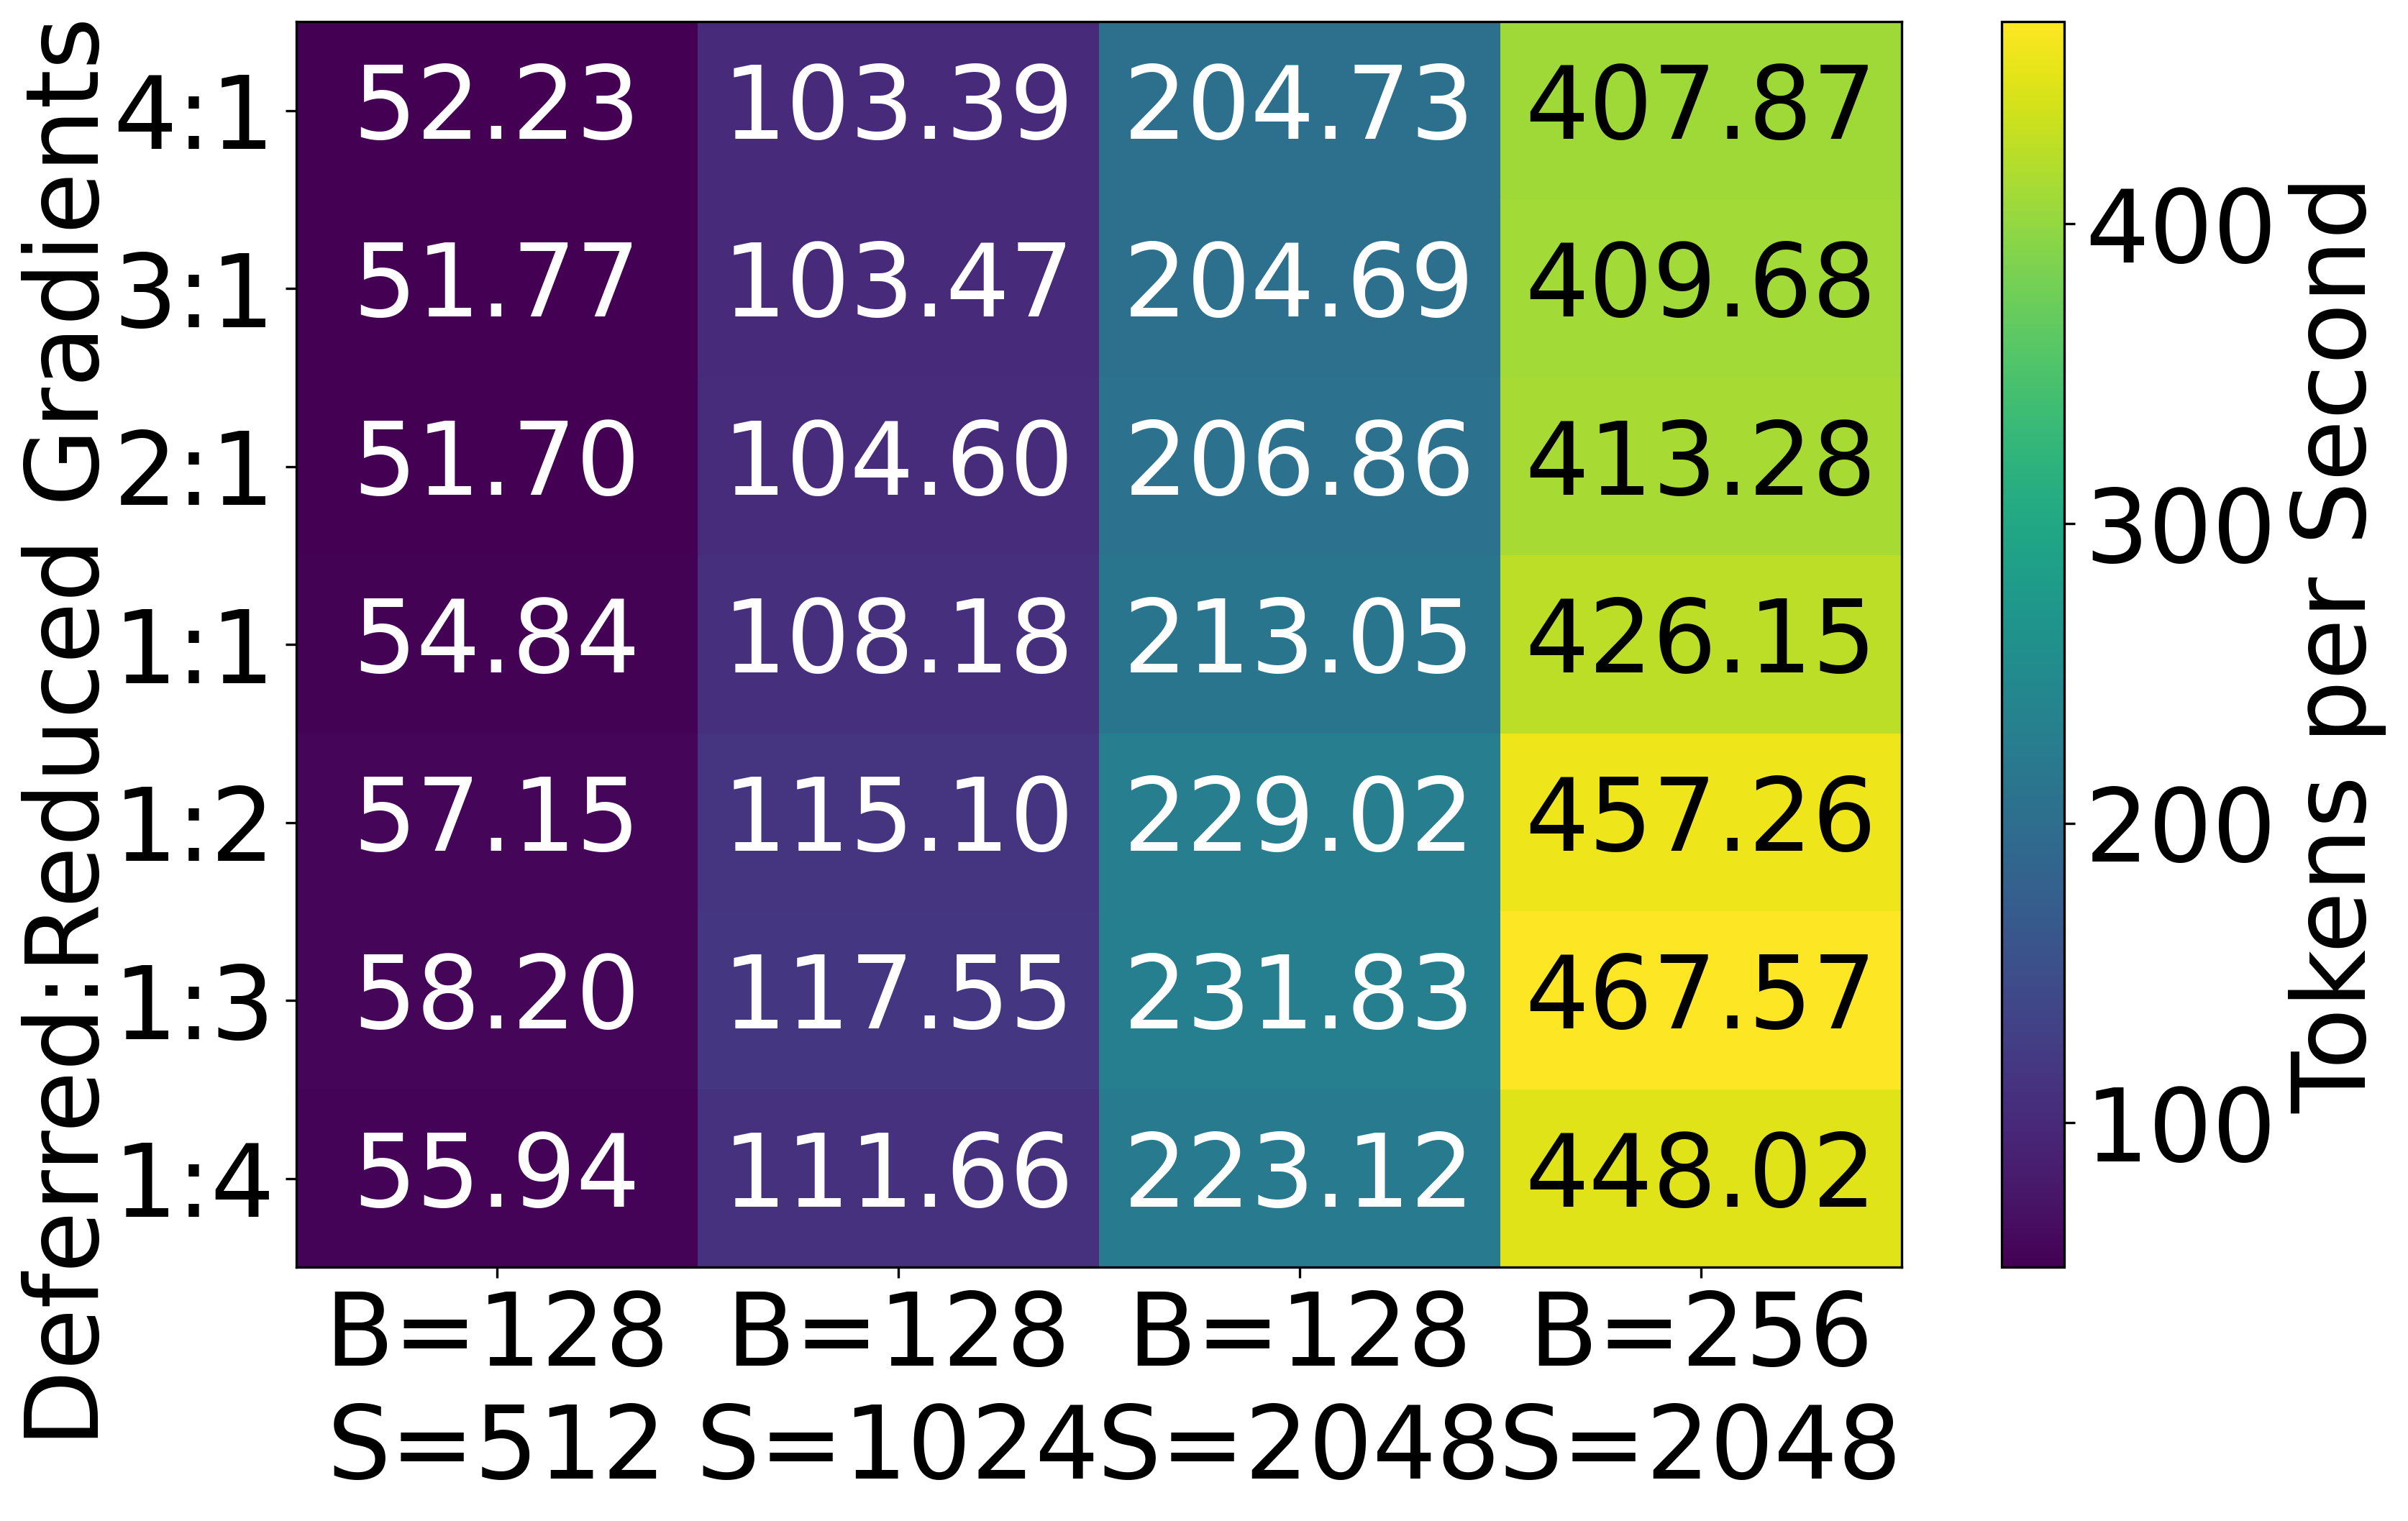
\includegraphics[width=\linewidth]{figures/strategy_4.0_ckpt_False_tokens_per_sec_heatmap.png}
    \vspace{-1.5em}
    \caption{Throughput (ZeRO-4)}
  \end{subfigure}
  \begin{subfigure}{0.48\linewidth}
    \centering
    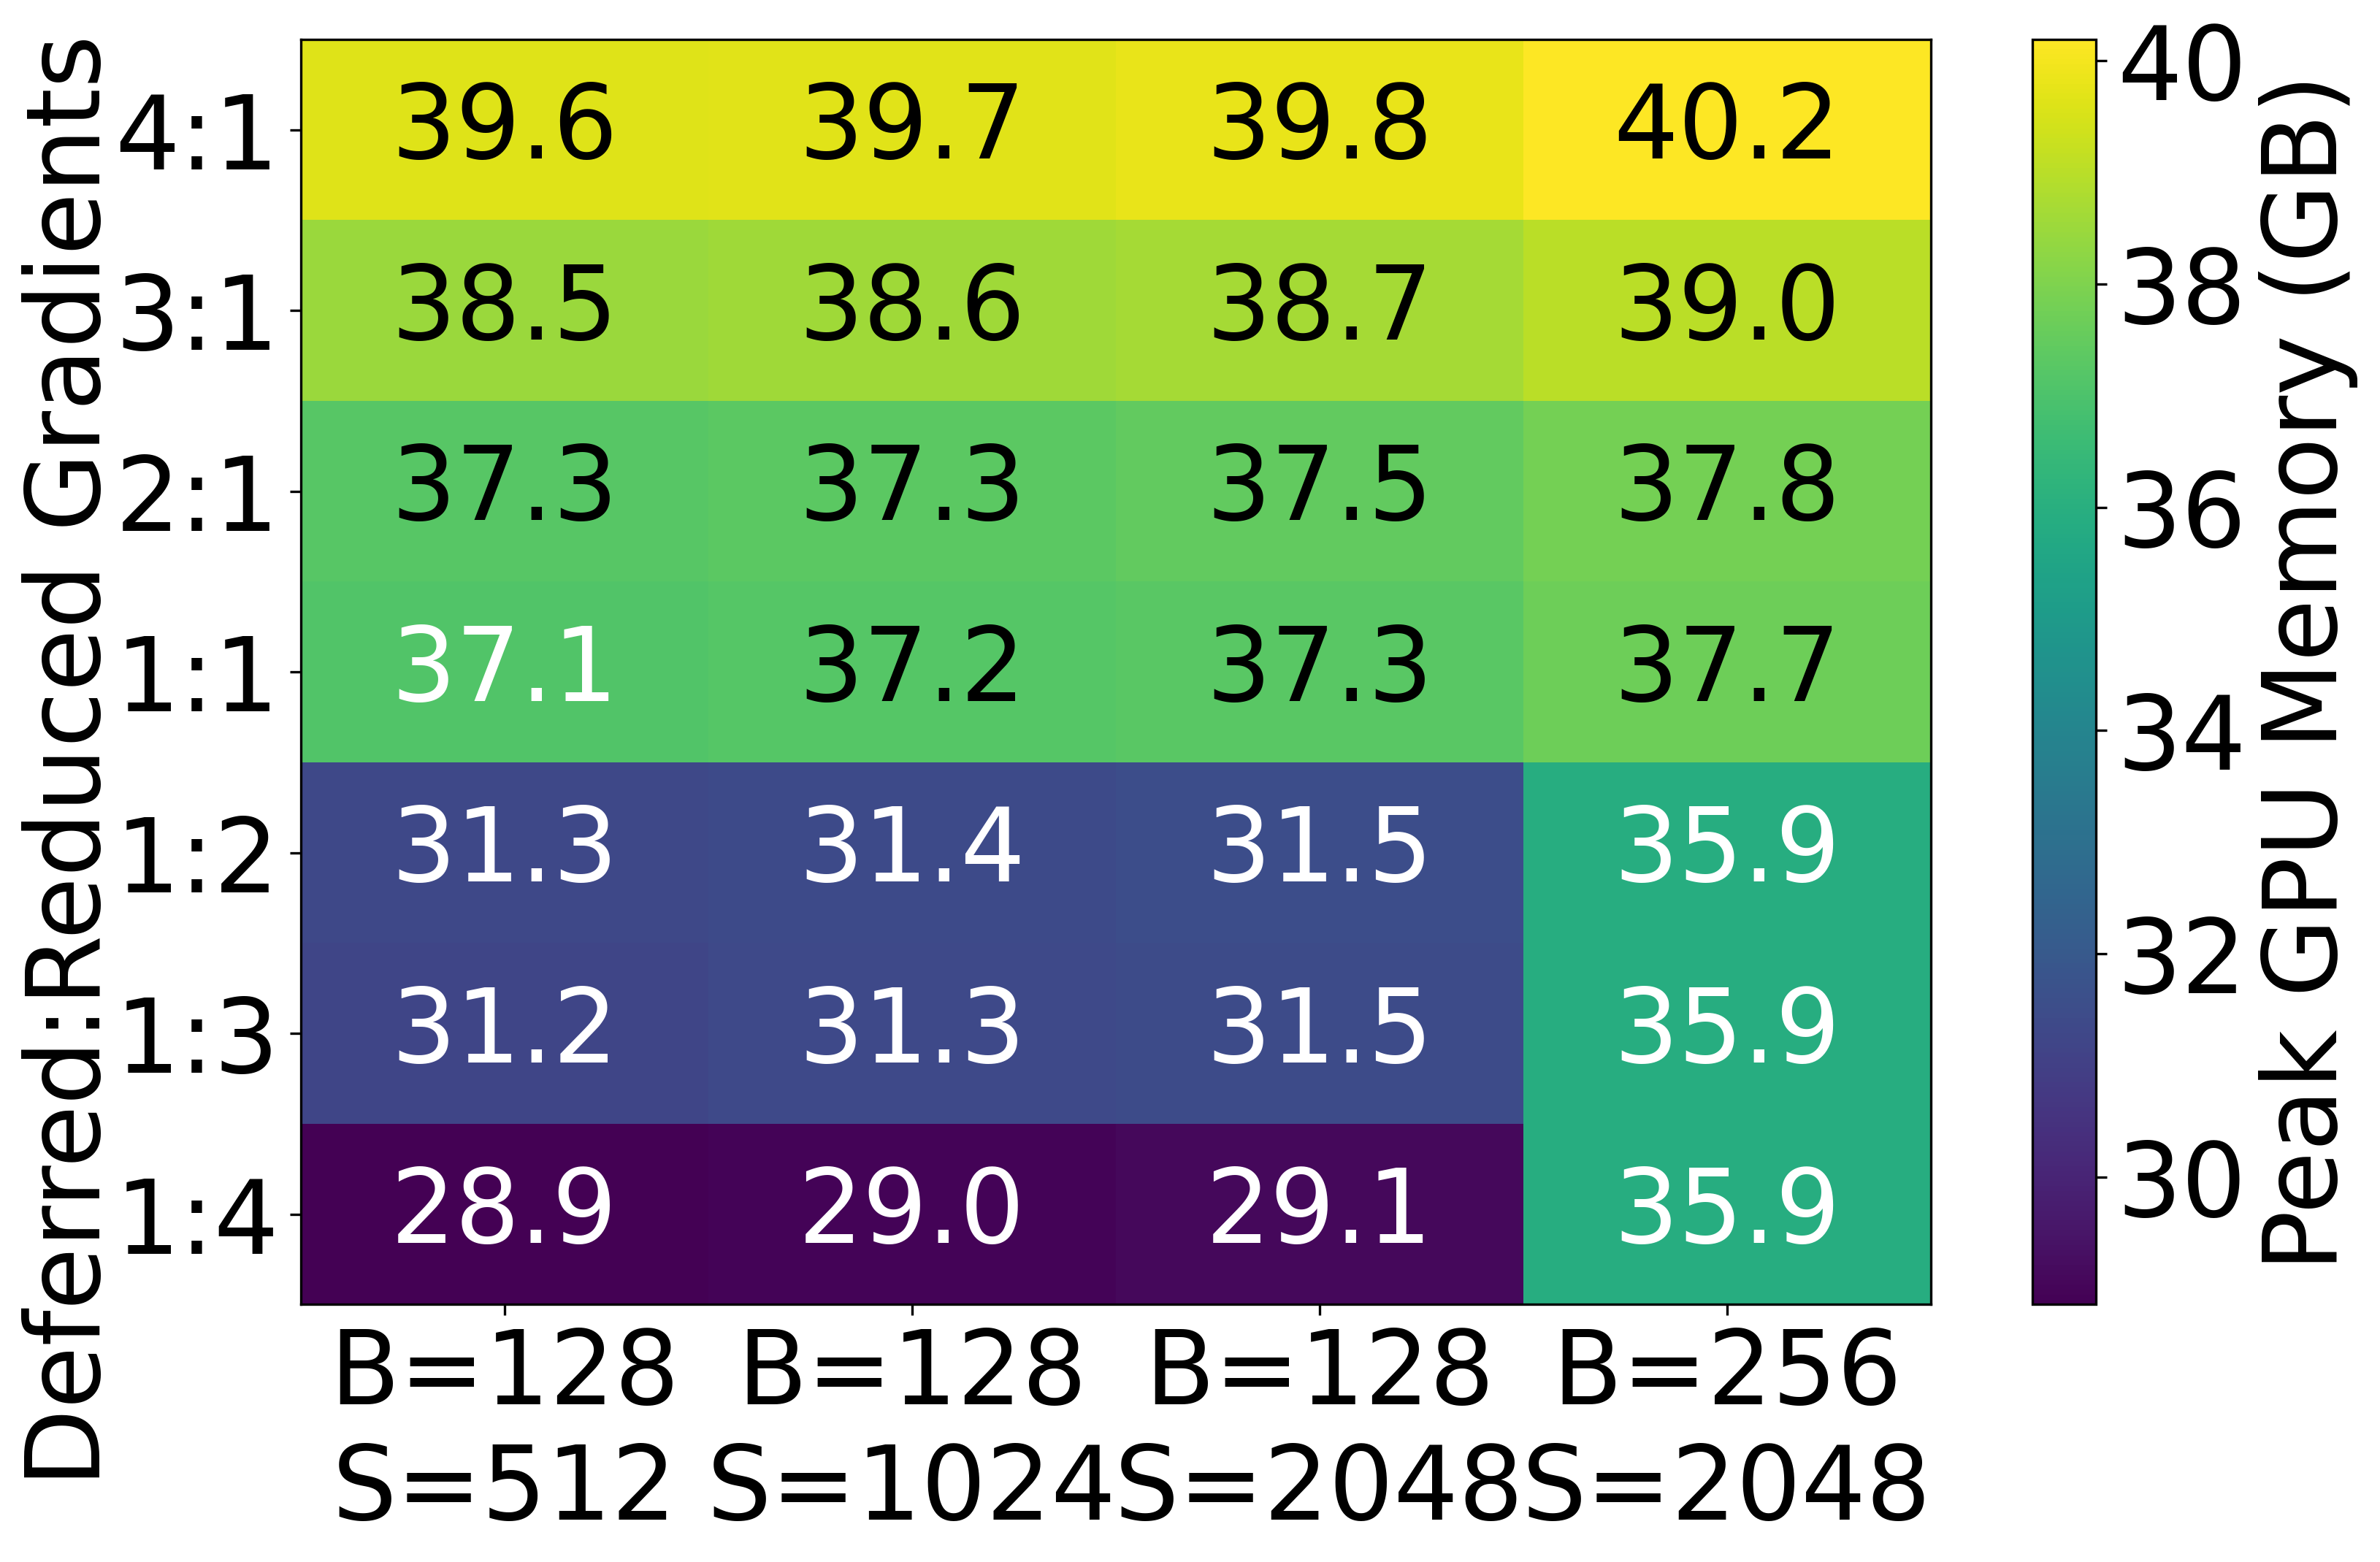
\includegraphics[width=\linewidth]{figures/strategy_4.0_ckpt_False_peak_gpu_mem_mb_heatmap.png}
    \vspace{-1.5em}
    \caption{Peak Memory (ZeRO-4)}
  \end{subfigure}
  \vspace{-1em}
  \caption{Configuration exploration of ZeRO-3.5 \& ZeRO-4.}
  \label{fig:zero_dse}
  \vspace{-.7em}
\end{figure}

As shown in Fig.~\ref{fig:zero_dse}(a), ZeRO-3.5's performance generally increases as the fraction of retained parameters grows, with larger gains under lighter computation loads. However, increasing the retained-parameter ratio can also raise peak memory usage. As shown in Fig.~\ref{fig:zero_dse}(b), when activation is small, the gathered parameters dominate peak memory, therefore, peak memory increases with the retained-parameter ratio. When activation is sufficiently large, the retained parameters can occupy the freed activation memory (Fig.~\ref{fig:FSDP}(c)), and retaining more parameters no longer increases peak memory.

Figure~\ref{fig:zero_dse}(c) shows that ZeRO-4 attains the best performance at a moderate deferred-gradient ratio (1:3). A low deferred ratio degenerates to ZeRO-3.5, while a high deferred ratio introduces excessive forward communication, which can overload the forward pass and reduce communication-computation overlap. When activation is small, peak memory grows with the deferred-gradient ratio due to more retained gradient buckets during backward (Fig.~\ref{fig:zero_dse}(d)). When activation is large enough, peak memory becomes less sensitive to the deferred-gradient ratio where both deferred gradient buckets and retained parameters can be accommodated in the released activation memory (Fig.~\ref{fig:FSDP}(d) \& \ref{fig:zero_comparison}(g)).

\subsection{Search Analysis}
\vspace{-.5em}
\label{sec:exp_search}

\name{}'s search process constructs a sequence of intermediate strategies that connect the initial strategy to the terminal one. As illustrated in Fig.~\ref{fig:zero_search}, under the data-monistic abstraction, each all-gather operation in ZeRO-3 creates a Weight Buffer CAT that collects weight shards from peer devices. The transition from ZeRO-3 to ZeRO-3.5 is a progressively delaying the release event of the Weight Buffer CAT during the backward pass until the corresponding forward layer is reached. At that point, the automatic management selects the Weight Buffer resident on the local device rather than all-gathering weights from other devices.

\begin{figure}[t]
  \centering
  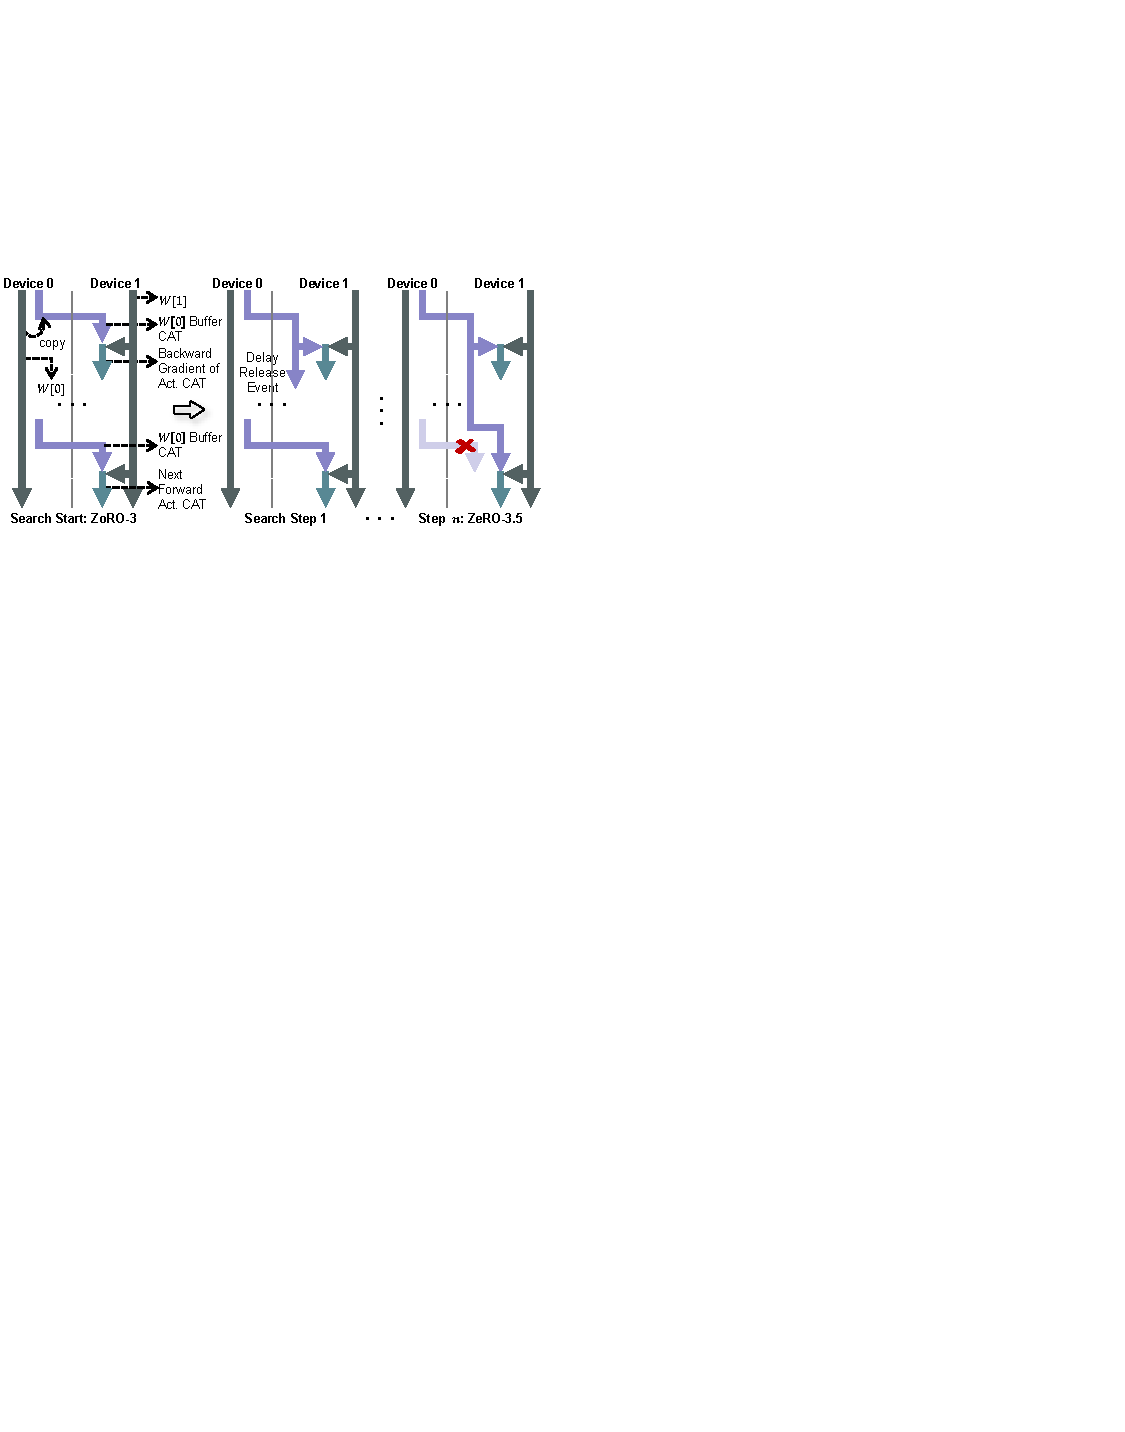
\includegraphics[width=1\linewidth]{figures/zero_search.pdf}
    \vspace{-1.5em}
  \caption{The intermediate plans during search from ZeRO-3 to ZeRO-3.5. A two-device example.}
  \vspace{-1.3em}
    \label{fig:zero_search}
\end{figure} 

In ZeRO search experiments, we set $\alpha=\beta=\gamma=1$ in Equation~\eqref{eq:event_potential} and $\delta=0.1$ in Equation~\eqref{eq:cat_potential}. Fig.~\ref{fig:comprehensive_search2} shows the distribution of event potential across CATs for ZeRO-3 and ZeRO-3.5. The changes of the Weight Buffer CAT are highlighted. It can be observed that two backward Weight Buffer CATs in the first accumulation step elongate their lifespans and replace the Buffer CATs of the subsequent forward results with a smaller accumulated potential.

\begin{figure}[h]
  \centering
  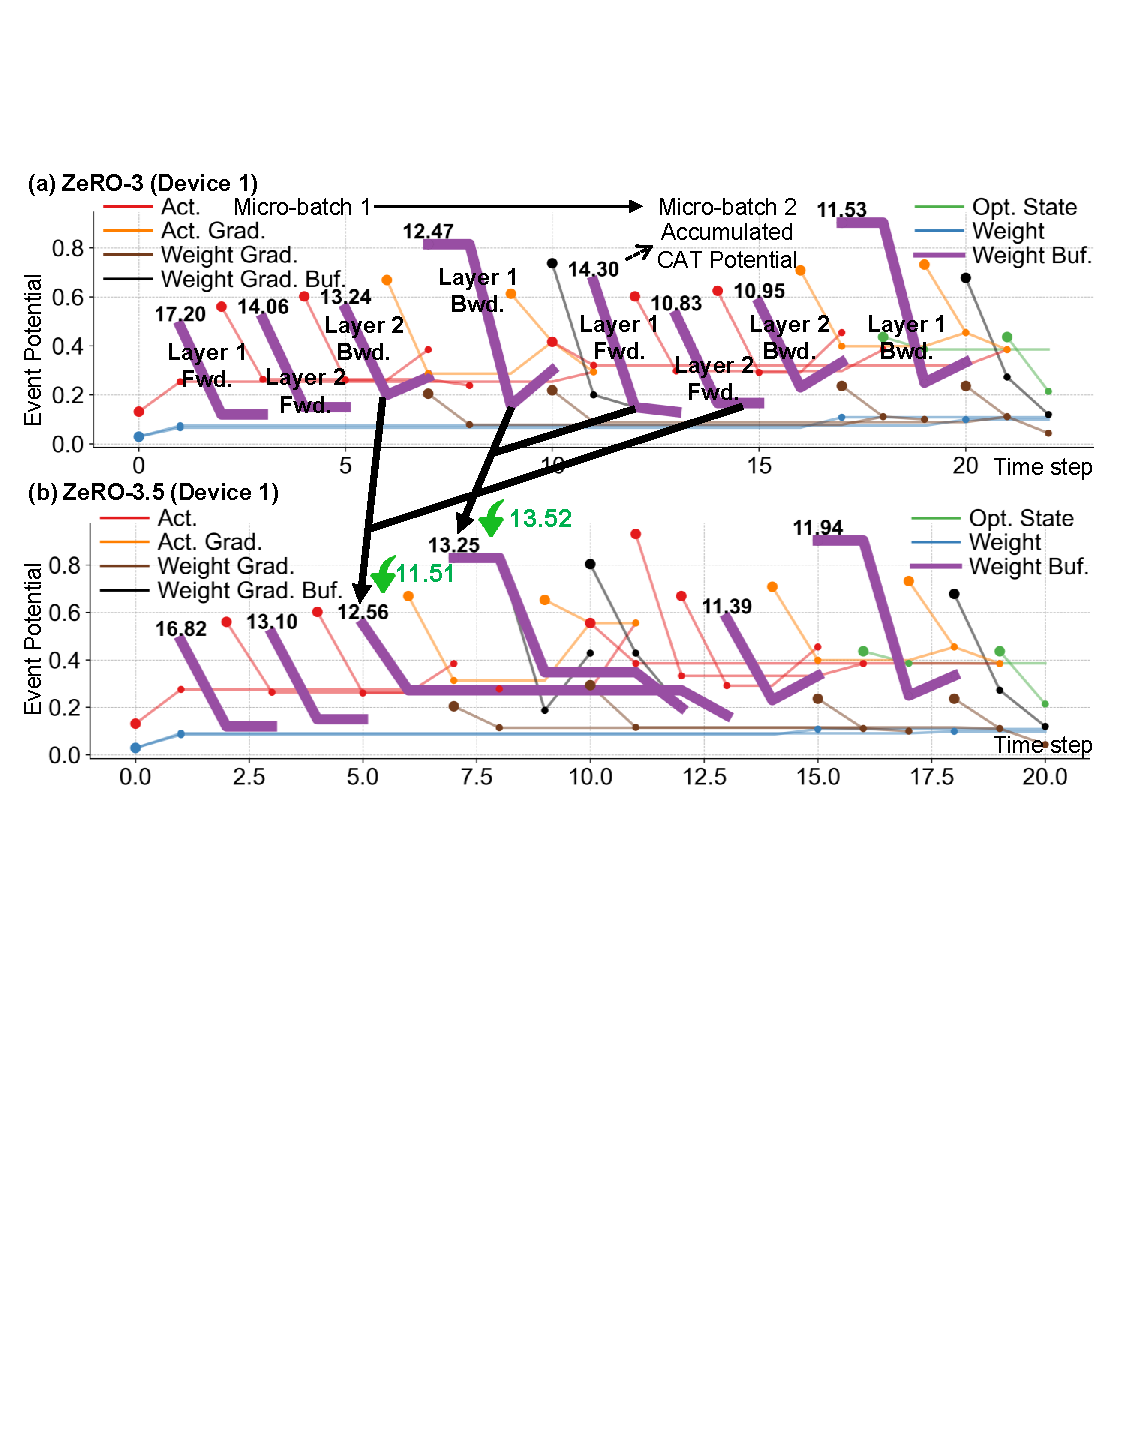
\includegraphics[width=1\linewidth]{figures/comprehensive_search_2.pdf}
    \vspace{-1.5em}
  \caption{Potential distributions for (a) ZeRO-3 and (b) ZeRO-3.5. Both strategies are illustrated using a 2-layer, 2-accumulation-step, 4-device configuration.}
  \vspace{-.5em}
    \label{fig:comprehensive_search2}
\end{figure}

Fig.~\ref{fig:zero_search_potential}(a) further plots the accumulated potential of each Weight Buffer CAT along the trajectory from ZeRO-3 to ZeRO-3.5 (The accumulated CAT potential of intermediate strategies). With the defined potential function, this transition constitutes a natural potential-descent process, causing the high reachability of ZeRO-3.5. In contrast, attaining ZeRO-4 is more challenging. As shown in Fig.~\ref{fig:zero_search_potential}(b), deferring the backward Weight Gradient Buffer to the subsequent forward pass does not yield a monotonically decreasing communication load for many layers, while the memory footprint grows with deferral and the attraction rules cannot be applied. Consequently, optimizing the Weight Gradient Buffer within automated search primarily serves to reveal promising directions rather than directly producing the final ZeRO-4 strategy.

\begin{figure}[t]
  \centering
  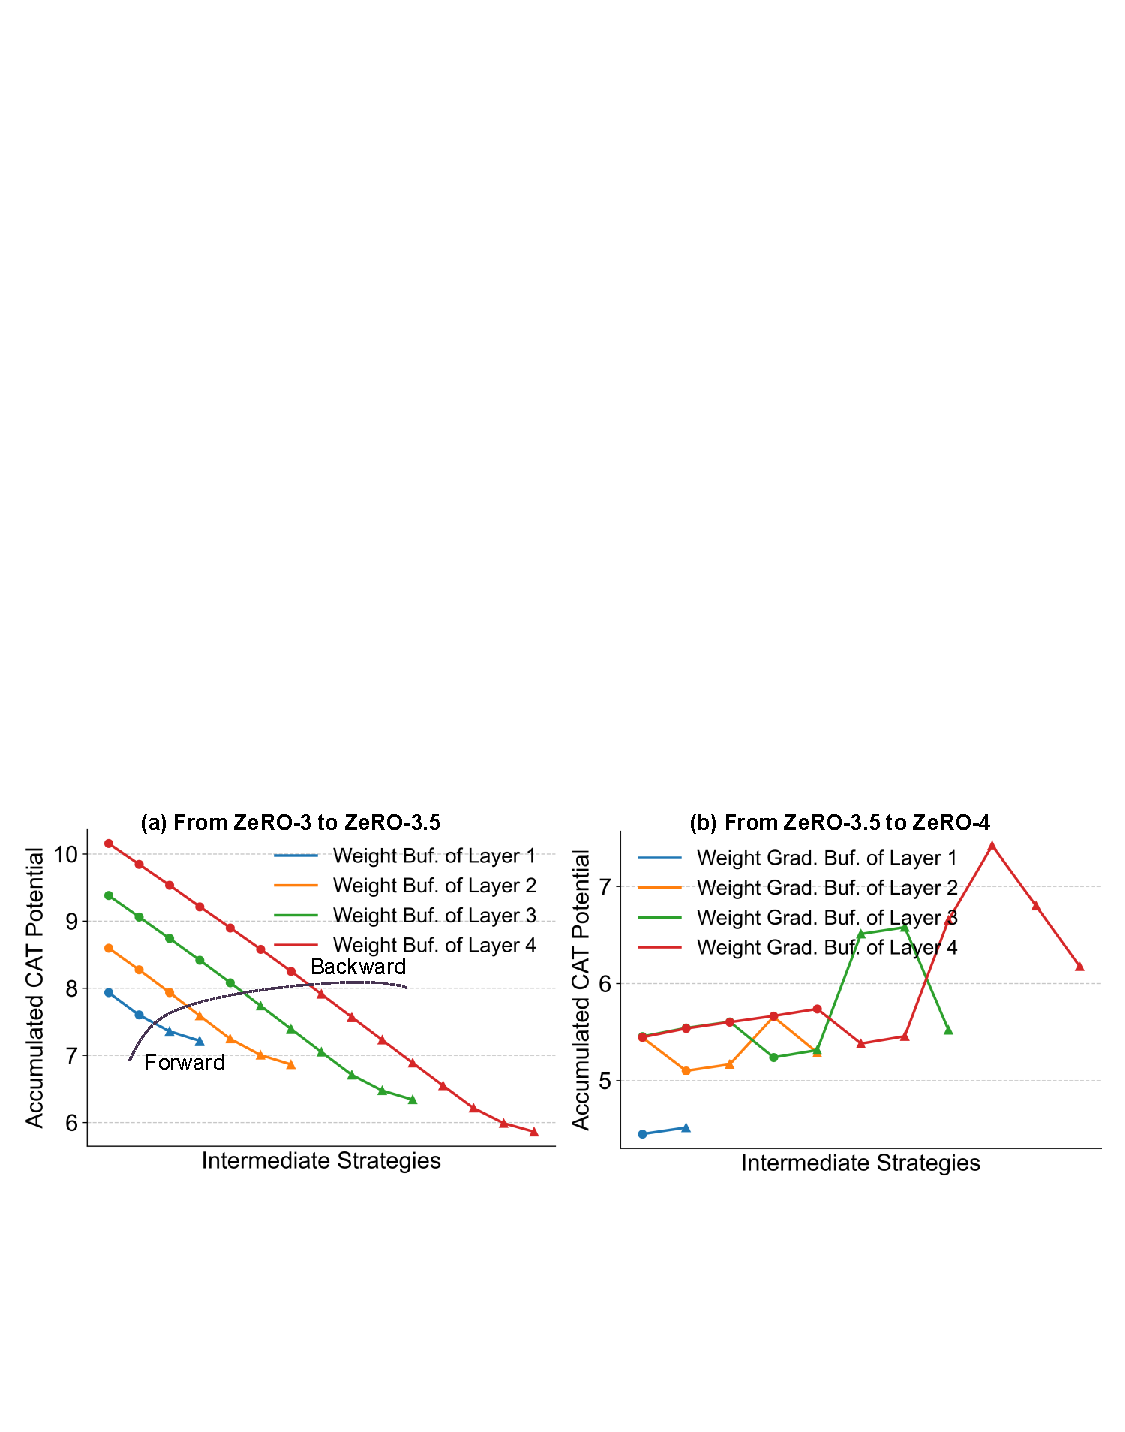
\includegraphics[width=1\linewidth]{figures/zero_search_potential.pdf}
  \vspace{-1.5em}
  \caption{Search trajectory of weight buffer CAT (a) from ZeRO-3 to ZeRO-3.5. (b) from ZeRO-3.5 to ZeRO-4.}
    \label{fig:zero_search_potential}
    \vspace{-.5em}
\end{figure} 

\vspace{-.5em}
\subsection{Comprehensive Exploration}
\label{sec:exp_offload}

\subsubsection{Seven Search Directions} 


\begin{figure}[t]
  \centering
  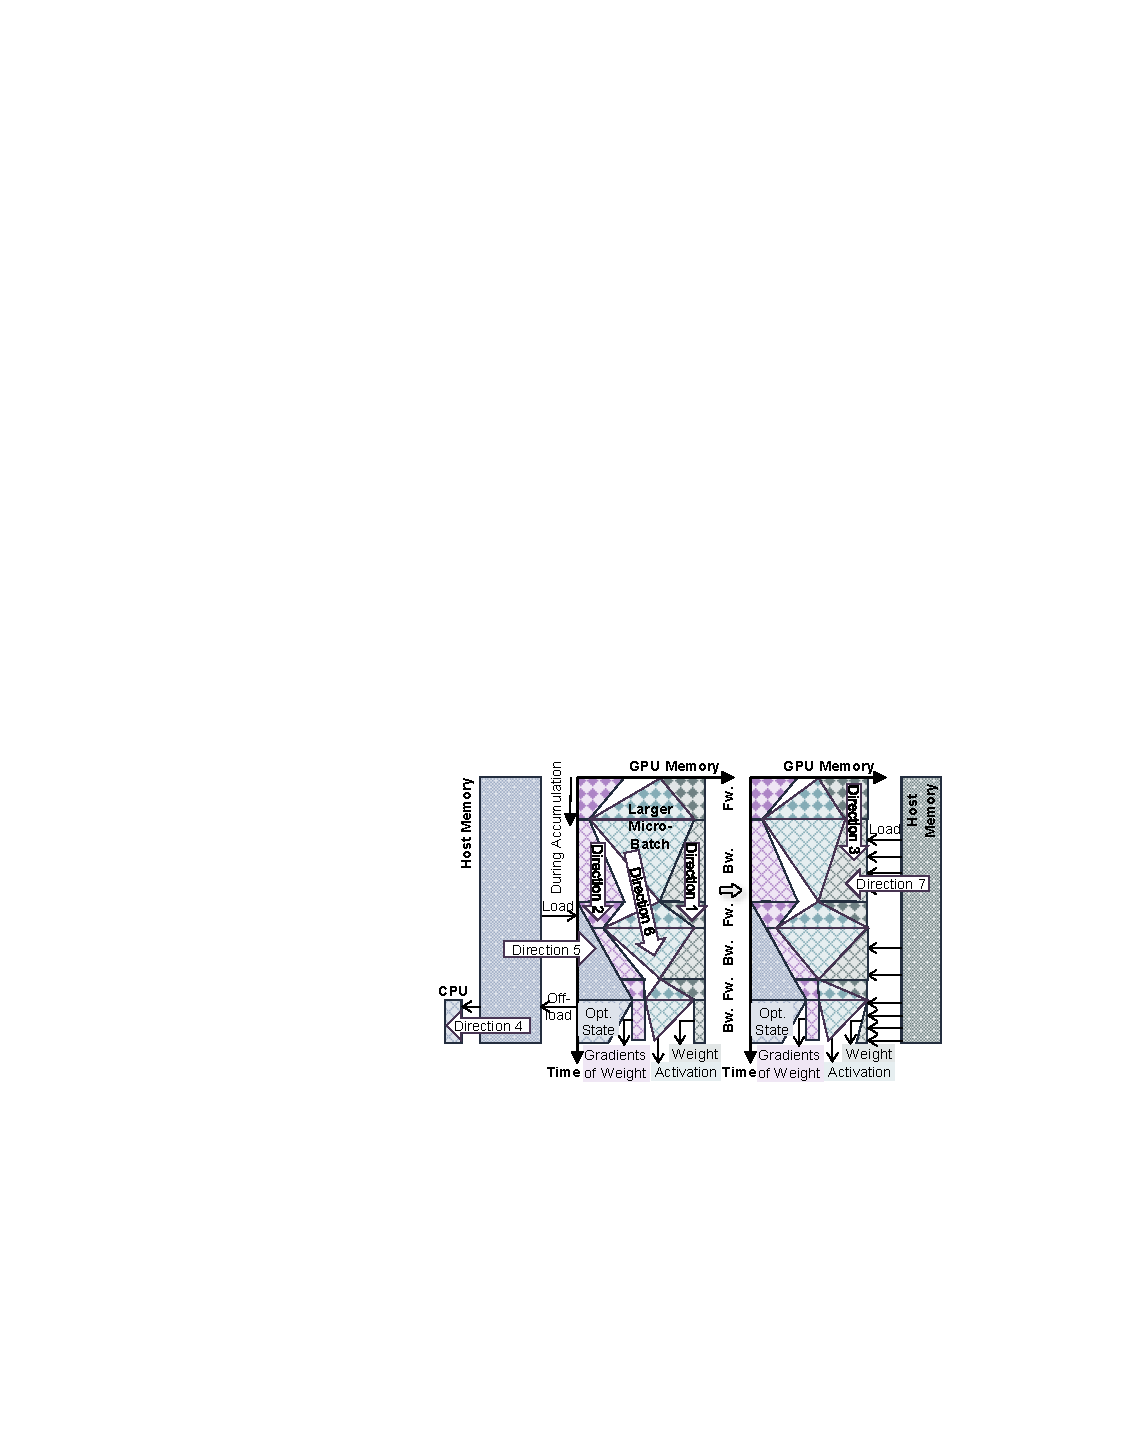
\includegraphics[width=0.9\linewidth]{figures/comprehensive_search_1.pdf}
  \vspace{-.5em}
  \caption{Comprehensive potential-descent directions discovered by \name{} starting from ZeRO-3. The seven directions span ZeRO improvement (1–3) and offload (4–7) optimizations, each targeting different computation-memory–communication trade-offs.}
   \vspace{-1.5em}
    \label{fig:comprehensive_search1}
\end{figure}


Starting from ZeRO-3, our data-centric potential-based search identifies seven meaningful scheduling optimization directions across various model and hardware configurations. These seven directions are comprehensively illustrated in Figure~\ref{fig:comprehensive_search1}. Directions 1 through 3 involve the GPU performing all storage and computation. \textbf{Direction 1} represents the ZeRO-3.5 strategy, i.e., delaying the release of backward weights. \textbf{Direction 2} represents the ZeRO-4 strategy, i.e., delaying the gradient reduce-scatter. \textbf{Direction 3} entails retaining a portion of forward weights for the backward pass, thereby increasing memory usage to reduce backward communication, which serves as an intermediate strategy between ZeRO-2 and ZeRO-3 (ZeRO-2.5). Directions 4 through 7 involve offload strategies:
\textbf{Direction 4:} Conventionally storing optimizer states in host memory (or SSD), with the CPU performing optimizer state updates.
\textbf{Direction 5:} Preloading optimizer states stored in host memory onto the GPU for updates.
\textbf{Direction 6:} Employing a larger micro-batch size before optimizer state preloading, and a smaller size after loading.
\textbf{Direction 7:} Off-loading weights to host memory. To the best of our knowledge, Direction 4 and 7 are existing plans.

\subsubsection{New Offload strategy} 



Guided by these directions, we propose a new offloading strategy, referred to as PTD-offload, that combines Directions 3 to 6. We deploy this design on real hardware and evaluate it against classical offload baselines across model sizes and hardware configurations, reporting throughput and memory usage to characterize its behavior.

\textbf{Baseline Offload (ZeRO-style).} Conventional offload techniques store optimizer states in host memory (DRAM) or SSD. During backpropagation, weight gradients on the GPUs are transferred to the host, the CPU applies the optimizer update (Direction 4), and the updated weights are sent back to the GPUs. End-to-end iteration time is frequently limited by host-device bandwidth and CPU throughput.

% to mitigate these bottlenecks, ZeRO-Infinity-style deployments sometimes provision multiple high-performance CPUs per GPU cluster.

\textbf{Preload-then-discard Offload Strategy (PTD-offload).} The strategy proposed by \name{} exploits available GPU memory to preload optimizer states onto the GPUs ahead of the final backward within a batch, performs the optimizer updates on the GPUs, and directly discards the optimizer states thereafter (Direction 5). In parallel, the CPU executes a redundant optimizer-state update (Direction 4), but the GPUs do not wait for the CPU results; they proceed to the next batch's gradient accumulation and later load the CPU-updated states when available. In addition, when optimizer states are not resident on the GPUs, the freed memory can be used to (1) increase the micro-batch size to better amortize communication and improve utilization (Direction 6), and (2) preserve forward weights for reuse in the backward pass (Direction 3).

\begin{figure}[t]
  \centering
  \begin{subfigure}{\linewidth}
    \centering
    
\includegraphics[width=0.9\linewidth]{figures/legend_offload.png}
    \vspace{-0.2em}
  \end{subfigure}
  \begin{subfigure}{0.49\linewidth}
    \centering
    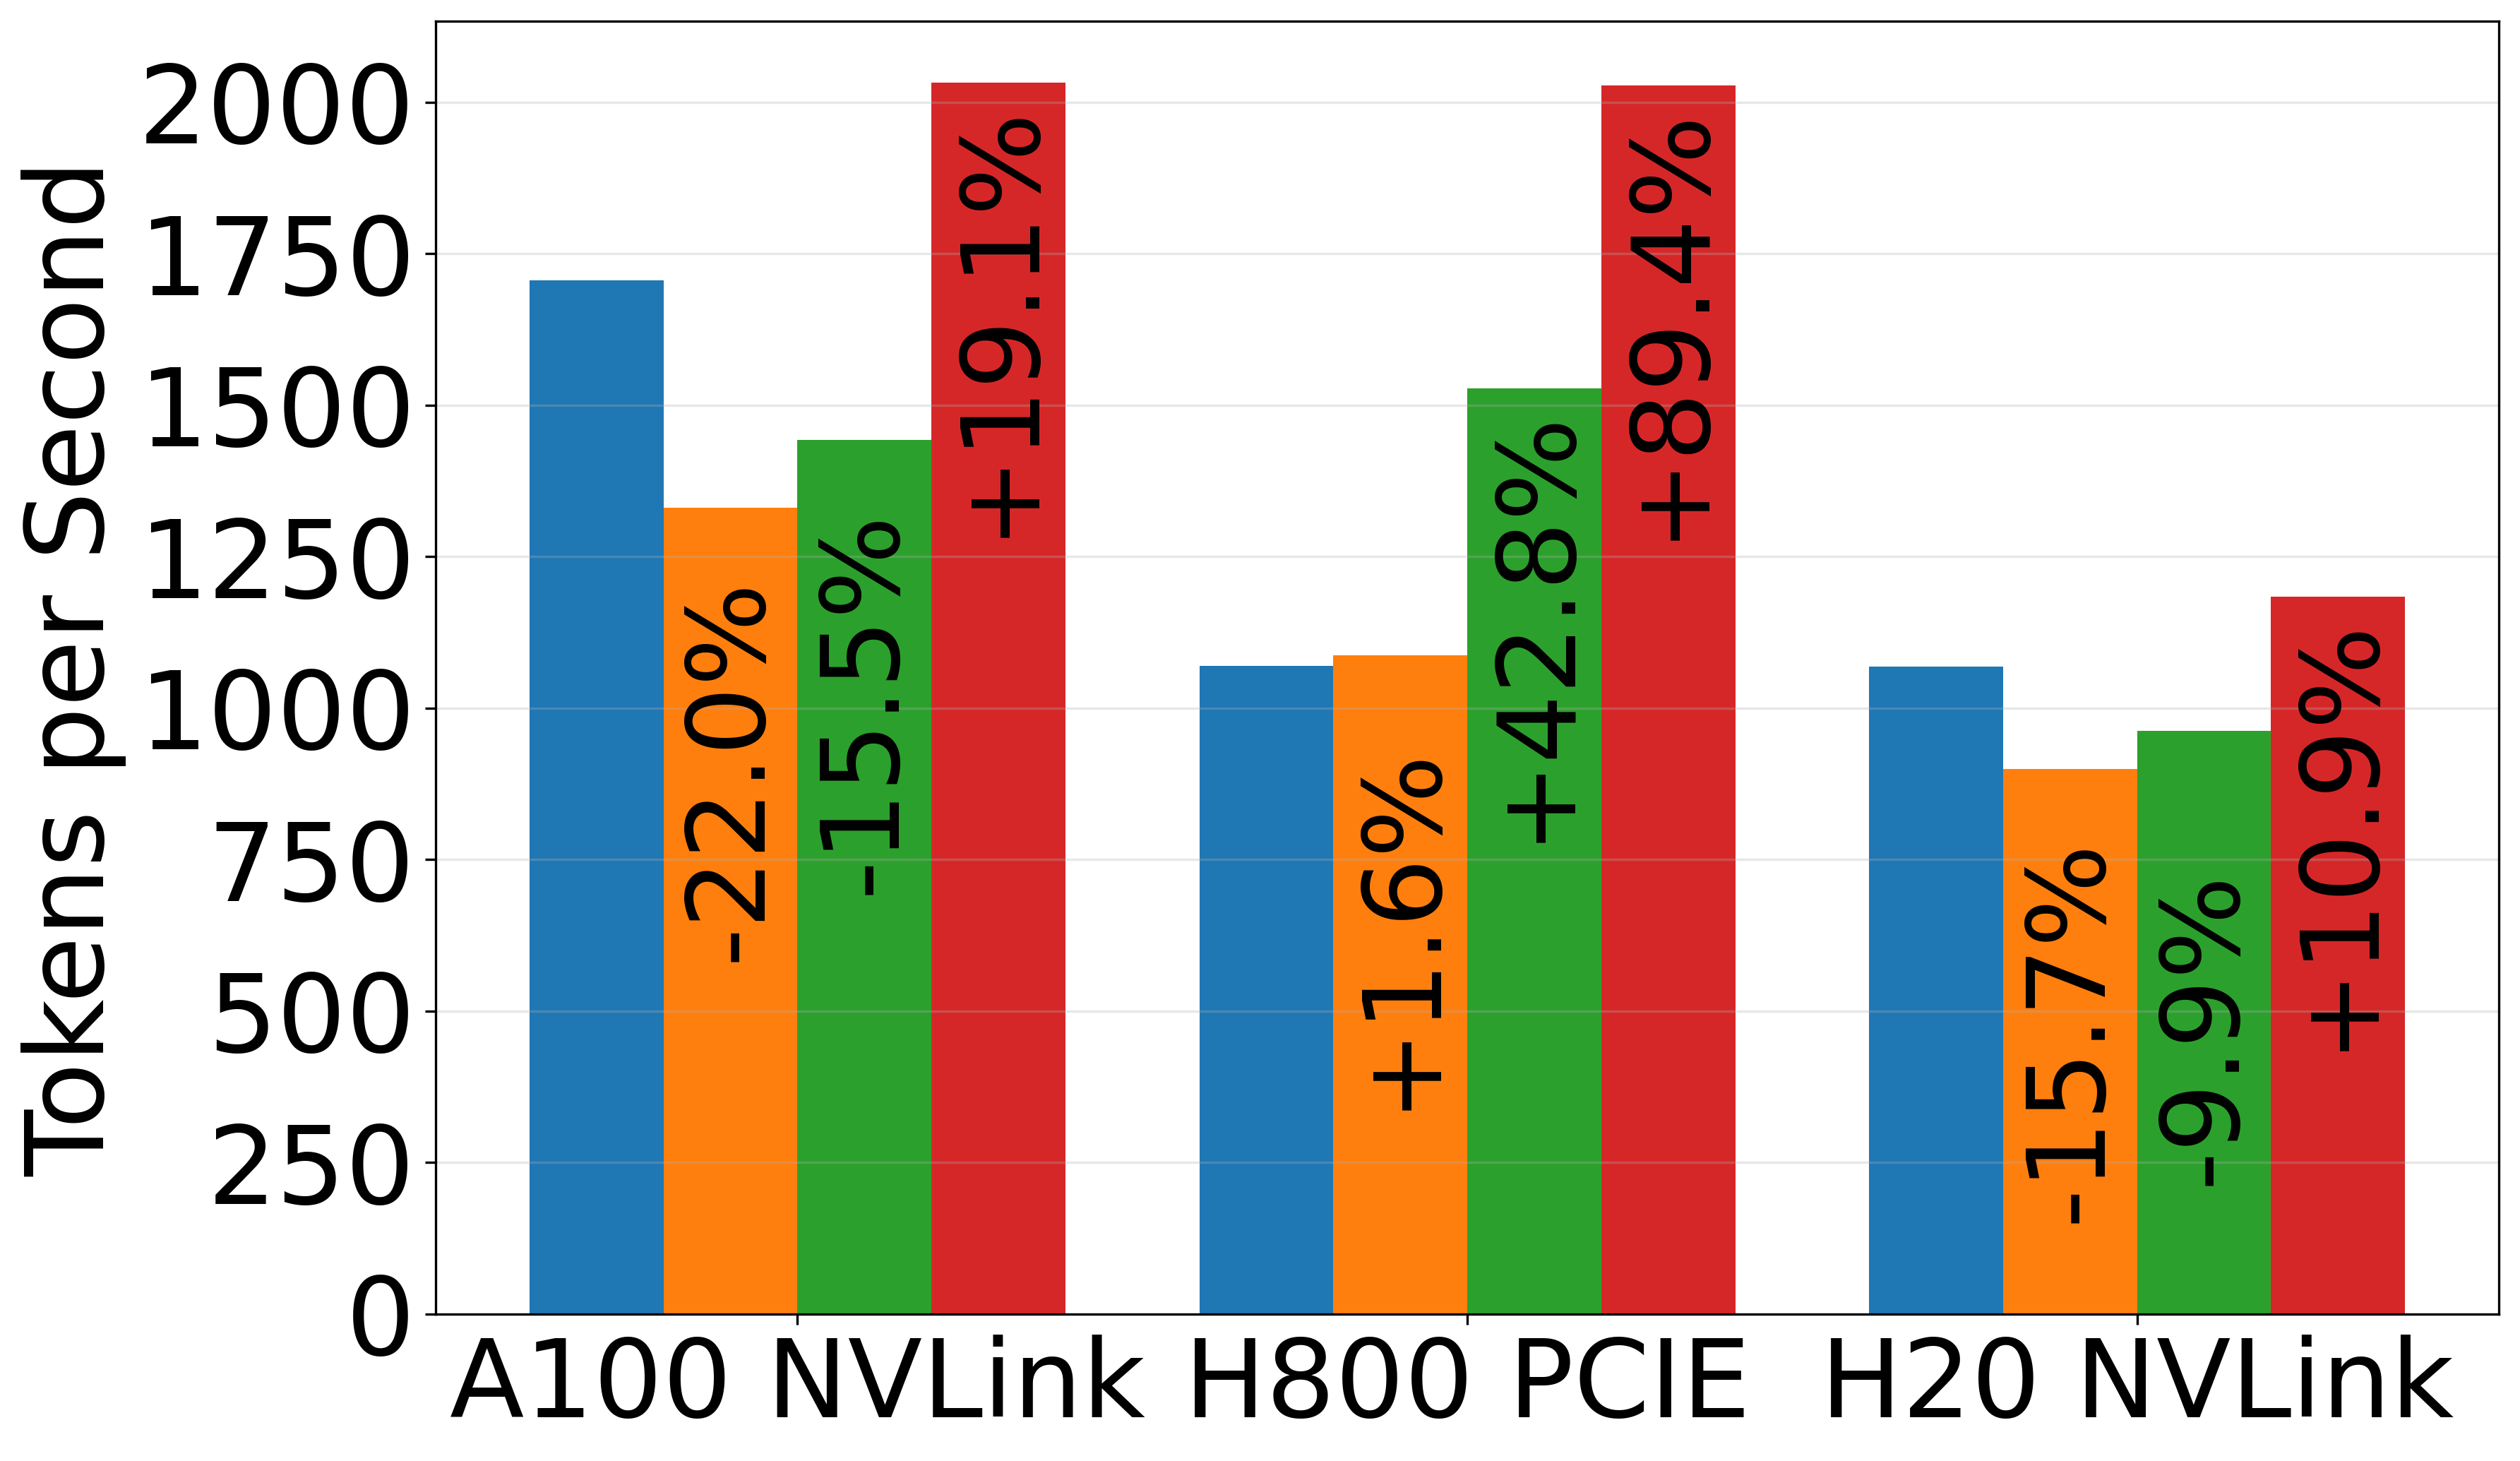
\includegraphics[width=\linewidth]{figures/offload_comparison_Qwen3-14B.png}
    \vspace{-1.5em}
    \caption{Qwen3-14B}
  \end{subfigure}
  \begin{subfigure}{0.49\linewidth}
    \centering
    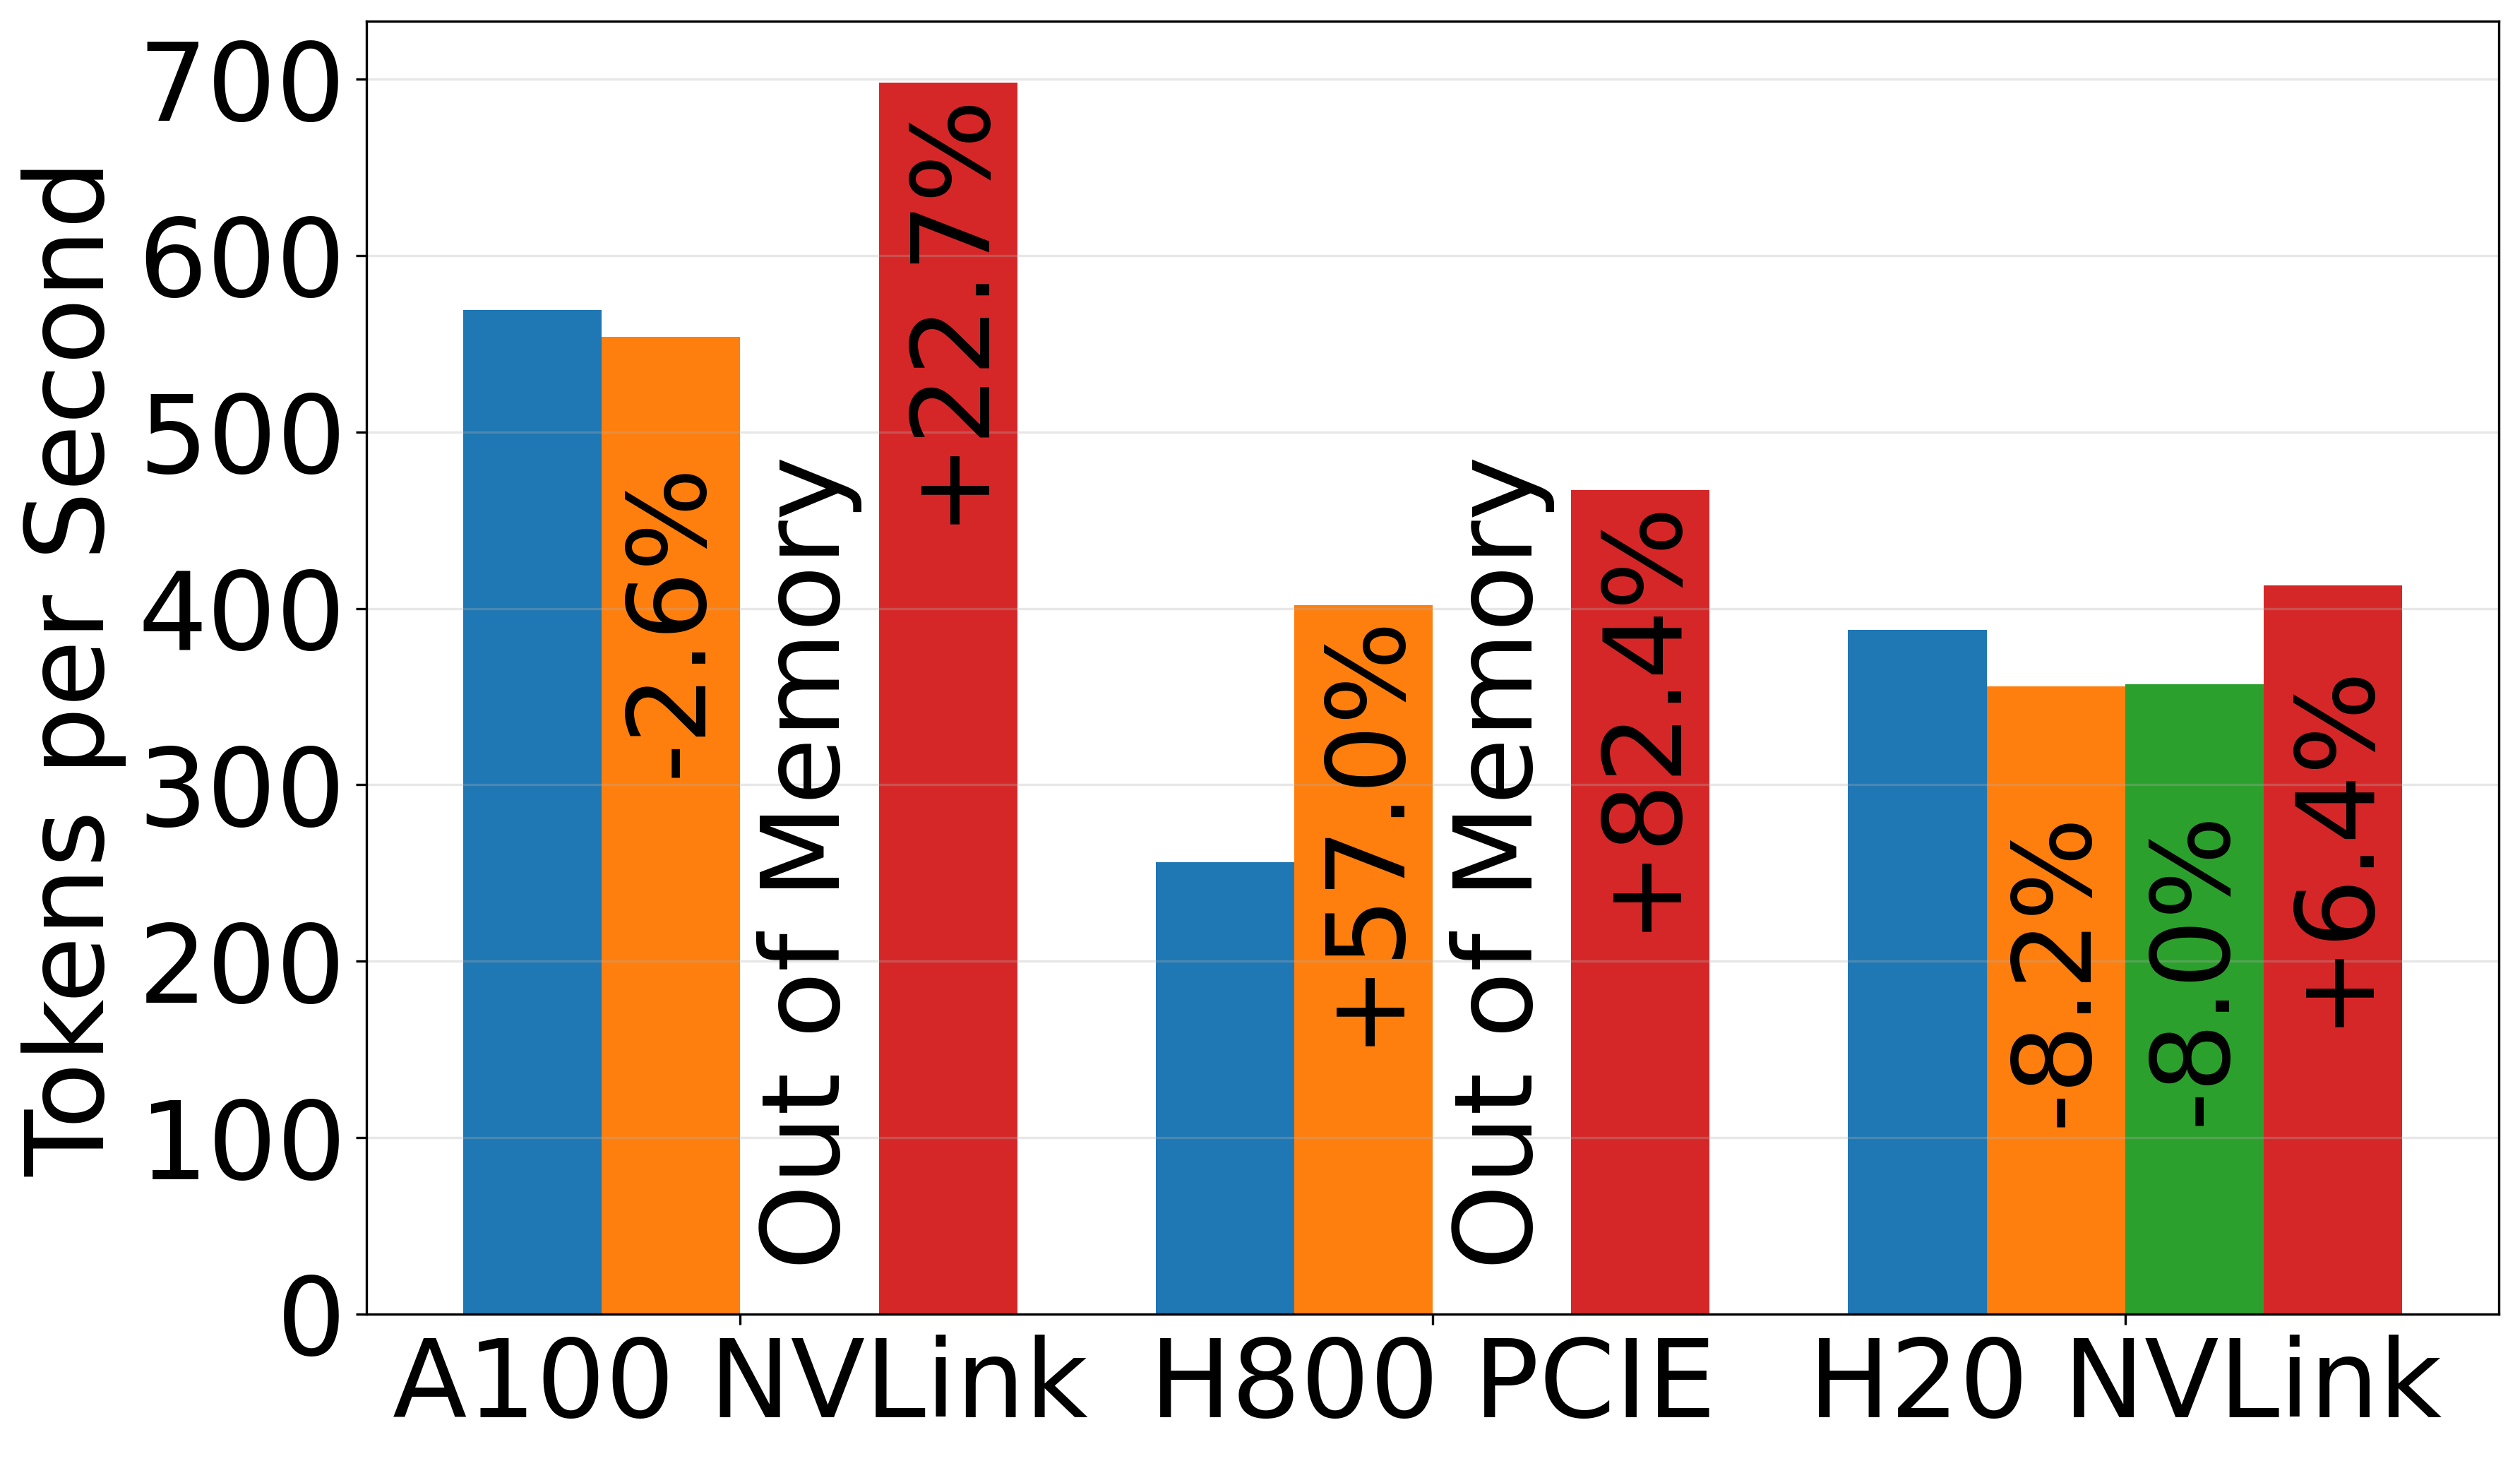
\includegraphics[width=\linewidth]{figures/offload_comparison_Qwen3-32B.png}
    \vspace{-1.5em}
    \caption{Qwen3-32B}
  \end{subfigure}
  \vspace{-.5em}
  \caption{Offload strategy comparison (relative to: ZeRO-3).}
    \vspace{-1.5em}
  \label{fig:off_load_strategy}
\end{figure}

Fig.~\ref{fig:off_load_strategy} compares our strategy with ZeRO-style offload strategies across two model sizes and three hardware configurations on 8 GPUs. We fix the per-GPU batch size and sequence length to 64 and 2048. For each configuration, we use the largest micro-batch size that does not cause OOM to maximize GPU utilization. Due to memory constraints, we enable gradient checkpointing for the 32B model, allowing a minimum batch size of $1$ under ZeRO-3. We do not include ZeRO-2, as it triggers OOM across all configurations.

In low-bandwidth configurations (e.g., H800-PCIe), ZeRO-3 throughput is limited by communication overhead. Offloading with ZeRO-3 enables larger batch sizes and can improve throughput. However, for the 14B model, the CPU weight update adds compute cost, yielding a small net improvement. In contrast, for the 32B model with gradient checkpointing, offloading enables a large increase in batch size (e.g., from 1 to 16), thereby improving throughput. PTD-offload combines the benefits of ZeRO and offloading: it begins with larger micro-batches and retained weights during early accumulation, then transitions to fully weight-sharded after preloading optimizer states. This segmented approach improves compute–communication overlap and avoids waiting on CPU-side optimizer updates, yielding significant performance gains across most settings. The exception is the H20 configuration, which offers higher bandwidth and larger memory, implying larger batch sizes and higher compute utilization.


\section{Related Works}


\textbf{Existing Training Optimizations.} The rapid growth of DNNs has driven the development of diverse parallelism plans for distributed training~\cite{duan2024efficient, verbraeken2020survey}. Common paradigms include DP, TP, PP, and SP~\cite{jacobs2023deepspeed}, and modern systems predominantly adopt hybrid parallelism~\cite{jain2020gems, park2020hetpipe}. For example, Megatron-LM~\cite{narayanan2021efficient} integrates DP, TP, and PP into a unified 3D parallelism framework. TeraPipe~\cite{li2021terapipe} combines SP with PP to facilitate finer-grained pipelining. With the escalating scale of models, research focus has shifted toward holistic co-optimization of computation, memory, and communication to maximize hardware utilization~\cite{zhu2025mist, zhuang2023optimizing}. To mitigate memory bottlenecks, ZeRO~\cite{rajbhandari2020zero} shard model states across DP devices, eliminating redundancy. Complementary techniques, such as offloading~\cite{ren2021zero} and recomputation~\cite{chen2016training}, further overcome memory constraints. Recent studies have deeply explored the interplay between parallelism and memory efficiency. In particular, Mist~\cite{zhu2025mist} introduces an automated system that co-optimizes memory reduction techniques with parallelism. Other studies examine memory-performance trade-offs in PP~\cite{kim2023bpipe, wan2025pipeoffload, qi2024pipeline}. In summary, synergistic optimization of computation, memory, and communication has become a cornerstone of contemporary large-scale model training.

\textbf{Parallelism Plan Search.} Finding an optimal parallelism plan for training is NP-hard~\cite{liu2024aceso}. Existing frameworks typically construct a parameterized search space from combinations of parallelization paradigms and then perform parameter search within that space~\cite{wang2019supporting, jia2019beyond, zheng2022alpa, tarnawski2021piper}. Early work such as FlexFlow~\cite{jia2019beyond} searches over SOAP (Sample-Operator-Attribute-Parameter) strategies. More recent systems like Alpa~\cite{zheng2022alpa} and Piper~\cite{tarnawski2021piper} adopt a hierarchical workflow: first determine a pipeline partition and then optimize intra-stage SPMD parallelism (staged SPMD). Tessel~\cite{lin2024tessel} focuses on micro-batch pipeline scheduling for a fixed placement. While effective, these methods typically search within a fixed space defined by manual templates or specific parallelism paradigms, limiting their ability to discover fundamentally new parallelism plans outside these predefined boundaries.

\textbf{Abstractions for Distributed Training.} To support more flexible plan, recent frameworks have introduced new abstractions. GSPMD~\cite{xu2021gspmd} uses tensor sharding annotations to drive compiler-based parallelization. nnScaler~\cite{lin2024nnscaler} proposes an operator-centric abstraction with primitives for placement, transformation, and ordering, enabling the expression of complex expert-designed strategies. However, these operator-centric views often treat data movement as a secondary effect of computation scheduling. In contrast, data-centric optimizations like BPipe~\cite{kim2023bpipe} and WeiPipe~\cite{lin2025weipipe} demonstrate the importance of explicit dataflow management. \name{} addresses this by adopting a data-monistic perspective, treating data movement and lifecycle as first-class citizens to enable the co-optimization of computation, memory, and communication.

\section{Conclusion}

In this paper, we present \name{}, a data-monistic framework that abstracts distributed training by unifying representations of data and computation. Through the novel concept of CATs and a set of data-centric primitives, \name{} enables the declarative specification of versatile parallelism plan space. We propose a constraint-based potential descent search algorithm that explores this vast strategy space, discovering parallelism plans that outperform existing solutions. \name{} focuses on high-level distributed scheduling and does not extend to micro-architectural optimizations tightly coupled with hardware, such as PagedAttention. In addition, more efficient runtime search algorithms for scheduling inference services could be further explored.

%-------------------------------------------------------------------------------
\bibliographystyle{plain}
\bibliography{ref.bib}

\appendix

\section{Data-Centric Primitives in \name{}}
\label{sec:all_primitives}

\begin{table*}[h]
\centering
\resizebox{\textwidth}{!}{%
\begin{tabular}{p{0.4\textwidth}p{0.6\textwidth}}
\toprule
Primitives                             & Usage \\ \midrule
\texttt{split(tensor, split\_vector, split\_tensors)}         & \texttt{tensor} represents the tensor to be partitioned. \texttt{split\_vector} represents the vector guiding how to partition \texttt{tensor}. \texttt{split\_tensors} are the result tensors. \\
\texttt{assign(tensor, device)}        & Assign \texttt{tensor} to \texttt{device}. \\
\texttt{copy(src\_tensor, device, dst\_tensor, path)} & Copy \texttt{src\_tensor} from its current device to \texttt{device}. The copied tensor on \texttt{device} can be accessed through the pointer \texttt{dst\_tensor}. \texttt{path} represents the copy path. \\
\texttt{cut(src\_tensor, device, dst\_tensor, path)} & Cut \texttt{src\_tensor} from its current device to \texttt{device}. The moved tensor on \texttt{device} can be accessed through the pointer \texttt{dst\_tensor}. \texttt{path} represents the cut path. After cut, \texttt{src\_tensor} will be freed from memory.        \\
\texttt{reduce(src\_tensors, device, dst\_tensor, path)} & Reduce \texttt{src\_tensors} into \texttt{dst\_tensor}. The reduction result will be placed on \texttt{device}. \texttt{path} represents the reduction path.     \\
\texttt{redirect(tensor1, tensor2, tensor3)} & Redirect the data dependencies between \texttt{tensor1} \& \texttt{tensor3} to \texttt{tensor2} \& \texttt{tensor3}.                                        \\
\texttt{order(event1, event2)}        & Enforce temporal order between \texttt{event1} and \texttt{event2}.  \texttt{event1} executes before \texttt{event2}.                                                                                      \\ \bottomrule
\end{tabular}%
}
\caption{Data-centric primitives for parallelization space construction in \name{}.}
\label{tab:primitives}
\end{table*}

\section{Details of ZeRO strategies}

FSDP is a widely-adopted data parallelism strategy that coordinates computation and data movement. It shards model parameters, gradients, and optimizer states across devices to reduce memory. During training, each device holds only a shard of the weights. For a forward pass, a device gathers the full parameters for the current layer, performs the computation, and then discards the full parameters, keeping only its shard. For the backward pass, gradients are computed locally and then reduced and sharded directly to the target devices using a reduce-scatter operation, avoiding redundant storage. This sharding strategy is often described in levels, inspired by the ZeRO (Zero Redundancy Optimizer) framework~\cite{rajbhandari2020zero}. ZeRO-1 shards optimizer states, ZeRO-2 adds gradient sharding, and ZeRO-3 (the typical FSDP implementation) shards parameters as well for maximum memory savings. Algorithm \ref{alg:fsdp} shows how \name{}'s primitives can represent the core of ZeRO-2/3. 

Figure \ref{fig:FSDP}(a-b) illustrates the approximate changes in storage and communication volume during training for ZeRO-2 and ZeRO-3. Figure \ref{fig:FSDP}(a) illustrates the storage and communication changes in ZeRO-2. During the forward pass, activation storage on each device increases as new activations are generated. In the backward pass, activations are consumed and released. In the final backward step of a batch, each device performs a reduce-scatter of gradients of weights with other devices to update its optimizer state and the corresponding weight shard; old weights can then be discarded. To balance communication load, ZeRO-2 typically performs an all-gather of new weights at the start of the next batch's first forward pass. Assuming each layer's forward computation takes one step and each device transmits one block of data per weight or gradient transfer, the communication volume per device during the first forward is 1 block/step. In the final backward, only gradients of weights are communicated, and since each backward layer takes about twice as long as a forward layer (2 steps), the average communication volume is 0.5 block/step. In practice, multiple gradient accumulation steps are performed; Figure \ref{fig:FSDP} shows only one accumulation, but this process is usually repeated many times and dominates training cost. During accumulation, since ZeRO-2 stores all weights on each device, only the reduce-scatter of weight gradients is needed during backward, with communication volume calculated as 0.5 block/step. ZeRO-3, by sharding the weights, achieves greater memory savings compared to ZeRO-2, as each device only stores a portion of the weights. However, during gradient accumulation, every forward and backward pass for each layer requires an all-gather operation to assemble the complete weights on each device before computation. Consequently, the average communication volume per device for both forward and backward passes is 1 block per step, which becomes the primary performance bottleneck in ZeRO-3. If a strategy could be found that achieves the memory savings of ZeRO-3 while approaching the communication efficiency of ZeRO-2, it would be highly valuable.

\section{Details and Concerns About Search Algorithm}
\label{sec:search_details}

1. Symmetry Constraints: To improve search efficiency and reduce highly irregular solutions, symmetry constraints can be introduced into the search algorithm. That is, CATs with symmetric constraint vectors are treated as equivalent, and their scheduling actions are bound together during the search process.

2. Collectivity and Individuality of Potential: In the main text, we describe the calculation of potential as a global property, implying that the potential landscape is identical for each CAT. However, this is not strictly the case. Some metrics that influence "potential," such as memory pressure or overall computation latency, are indeed global. However, each CAT may also be subject to individualized constraints that exert personalized pressure, such as the requirement to arrive at a specific device before a certain event to synchronize with another CAT. As the event approaches, the pressure for the CAT to flow toward that device increases. Therefore, the movement of each CAT is not determined solely by the global potential.

3. In the absence of the hole mechanism described in the main text, it is not possible to constrain non-domain strategy spaces. Thus, by default, our search algorithm allows free exploration of these strategy spaces.

4. The search algorithm should be guided by certain heuristics. For example, in the absence of pressure-driven guidance, a CAT may simply remain on its current device without being released. Such heuristics can help the algorithm discover anticipated strategy optimization directions.

5. Two-level Heuristic Descent: In theory, it is possible to treat the constraint vector of a CAT as a whole and perform heuristic descent on it. However, finding the optimal descent direction would require enumerating all possible next-step transformations of the constraint vector, which is computationally infeasible due to the combinatorial explosion when multiple event points are involved. To address this, we adopt a two-level heuristic descent approach. At the first level, we perform local heuristic descent for each event point, identifying the optimal descent direction for each (i.e., applying a coordinate descent algorithm to the constraint vector). At the second level, we combine these locally optimal descent directions to determine the overall optimal descent direction for the entire constraint vector.

6. It is not accurate to state that the search process continuously refines the strategy space, as the potential descent algorithm merely iterates from one strategy solution to another without altering the strategy space itself. However, it is correct to say that the process of writing primitives refines the strategy space. In addition, a refinement engine exists within the search algorithm—using techniques such as constraint propagation—to prune the strategy space.

\section{Implementation Details}
\label{sec:implementation_details}

%%%%%%%%%%%%%%%%%%%%%%%%%%%%%%%%%%%%%%%%%%%%%%%%%%%%%%%%%%%%%%%%%%%%%%%%%%%%%%%%
\end{document}
%%%%%%%%%%%%%%%%%%%%%%%%%%%%%%%%%%%%%%%%%%%%%%%%%%%%%%%%%%%%%%%%%%%%%%%%%%%%%%%%

%%  LocalWords:  endnotes includegraphics fread ptr nobj noindent
%%  LocalWords:  pdflatex acks
